% Compile with:
%		pdflatex --shell-escape filename

%%%%%%%%%%%%%%%%%%%%%%%%%%%%%%%%%%%%%%%%%%%%
% Select to have report for SAAB or Chalmers
\def\saab{true}

\ifdefined\saab
	% Use template for the SAAB-report
	\documentclass[english,twoside,notitlepage]{reportsaab} % Full report
	%\documentclass[english,twoside,notitlepage,draft]{reportsaab} % No figures - faster
	% Get rid of nasty whitespace between paragraphs
	\setlength{\parskip}{0ex}

\else
	% Use template for the Chalmers-report
	\documentclass[a4paper]{report}
\fi

% Optional resolution usage:
%\opt{res300}{\includegraphics[width=200pt]{fig/introduction/300/figur}}
%\opt{res72}{\includegraphics[width=200pt]{fig/introduction/72/figur}}

% Include packages and commands
%%%%%%%%%%%%%%%%%%%%%%%%%%%%%%%%%%%%%%%%%%%%%%%%%%
% When making a high-res pdf for printing, use
% the following define. Changes resolution and colour
% of hyperlinks.

\def\printable{true}

%%%%%%%%%%%%%%%%%%%%%%%%%%%%%%%%%%%%%%%%%%%%%%%%%%
% If the following define is commented,
% not all packages will be used, resulting in
% a faster compile.

\def\generatefull{true}

%%%%%%%%%%%%%%%%%%%%%%%%%%%%%%%%%%%%%%%%%%%%%%%%%%
% Mandatory packages

% Language
\usepackage[english,swedish]{babel}

% Modern font encoding
\usepackage[utf8]{inputenc}

% Really good for quoting text's, source code, etc
\usepackage{listings}
% For multiple rows within tables
\usepackage{multirow}
% For good-looking figures side by side
\usepackage{subfig}

\usepackage{units}

% Nice math output
\usepackage{amsmath}

\usepackage{MnSymbol}

\usepackage{ctable}

% Custom toc-depth for different parts of the document
\usepackage{tocvsec2}

%\usepackage{txfonts} % Screws up all the equations, using upgreek for straight \mu:s instead
\usepackage{upgreek}

% Packages that are not crucial may be put in here to speed things up.
% (Ie, packages dealing only with aesthetics
\ifdefined\generatefull
	% Not sure what this does
	\usepackage{ae}
	% Adjusts textblocks in subtle ways (looks better)
	\usepackage{microtype}		
	% Included in the cls-file or not 'yet' needed
	%\usepackage{lipsum}
	%\usepackage[T1]{fontenc}


	% Nice captions
	\usepackage{caption}
	\captionsetup{margin=10pt,font=small,labelfont=bf}
	\captionsetup[table]{position=top}

\fi
%%%%%%%%%%%%%%%%%%%%%%%%%%%%%%%%%%%%%%%%%%%%%%%%%%
% LaTeXDraw
%\usepackage[usenames,dvipsnames]{pstricks}
%\usepackage{epsfig}
%\usepackage{pst-grad} % For gradients
%\usepackage{pst-plot} % For axes
% Doesn't work. Using .eps instead.


%%%%%%%%%%%%%%%%%%%%%%%%%%%%%%%%%%%%%%%%%%%%%%%%%%
%	pdflatex setup
% 	Use with:
%		pdflatex --shell-escape filename

%\usepackage[pdftex]{color,graphicx} % Already in class-file for logo
\usepackage{epstopdf}

%%%%%%%%%%%%%%%%%%%%%%%%%%%%%%%%%%%%%%%%%%%%%%%%%%


%% Check if we are building for the web or for printing
\ifdefined\printable
	\def \backref {false}
	\usepackage[res300]{optional}
\else
	% Printable was not defined, therefore:
	%	Set settings according to the web
	\def \backref {true}
	\usepackage[res72]{optional}
\fi

%%%%%%%%%%%%%%%%%%%%%%%%%%%%%%%%%%%%%%%%%%%%%%%%%%
% Biblatex will soon be the standard citations-package
\usepackage[
%		sorting=nyt, %previous
		sorting=none,
		hyperref=auto,
	%	style=authoryear-icomp-tt, % Special style to avoid broken authoryear
%		style=authoryear, %previous
		style=numeric-comp,
%		citestyle=authoryear,
		doi=false,
		isbn=false,
		bibstyle=numeric,
%		autocite=footnote, %previous
		autocite=plain,
		backref=\backref
	]{biblatex}

\bibliography{references}


%%%%%%%%%%%%%%%%%%%%%%%%%%%%%%%%%%%%%%%%%%%%%%%%%%
% Hyperref
\usepackage[pdfauthor={Richard Abrahamsson, Anders Bennehag},%
pdftitle={S-band Multi-function Down-converter GaAs MMIC},%
pdftex]{hyperref}
% Hypcap makes hyperlinks really point to the picture,
% not to the caption below
\usepackage[all]{hypcap} 

\definecolor{black}{rgb}{0.0,0.0,0.0}
\definecolor{darkblue}{rgb}{0.0,0.0,0.5}
\ifdefined\printable
	% Make links black (better for printing)
	\hypersetup{pdftex,colorlinks,breaklinks,
		linkcolor=black,urlcolor=black,
		anchorcolor=black,citecolor=black}
\else
	% Printable was not defined, therefore: Set settings according to the web
	\hypersetup{pdftex,colorlinks,breaklinks,
		linkcolor=darkblue,urlcolor=darkblue,
		anchorcolor=darkblue,citecolor=darkblue}
\fi


%%%%%%%%%%%%%%%%%%%%%%%%%%%%%%%%%%%%%%%%%%%%%%%%%%
%Custom commands
\newcommand{\includerect}[2]{\includegraphics[trim=50 60 40 60, clip, width=#1]{#2}}
\newcommand{\includesmith}[2]{\includegraphics[trim=60 40 60 50, clip, width=#1]{#2}}
\newcommand{\mum}{$\upmu$m}
\newcommand{\disclaimer}{ Temperature at \unit[25]{$^\circ$C} and no parameter spread applied.}
\newcommand{\scalemum}{ Dimensions in \mum.}
\newcommand{\nf}{\emph{NF}}

\usepackage{ifthen}
 
\newcommand{\newevenside}{
	\ifthenelse{\isodd{\thepage}}{\newpage}{
	\newpage
        \phantom{placeholder} % doesn't appear on page
	\thispagestyle{empty} % if want no header/footer
	\newpage
	}
}

% Add Contents to pdf-bookmarks
\addtocontents{toc}{\protect{\pdfbookmark[0]{\contentsname}{toc}}}

% Set a proper header separation
\addtolength{\headsep}{20pt}
\begin{document}

	% Title page, abstract and foreword
	\ifdefined\saab
		\pagenumbering{arabic}
		\setcounter{page}{1}
	\fi
	
	\title{S Band Multi-function Down-converter MMIC \\ Master's Thesis}
\author{OEGPUD Richard Abrahamsson, Anders Bennehag}
\titlepageauthor{Richard Abrahamsson \and Anders Bennehag}
\date{\mytoday}
%\date{2010-12-01}
\documenttype{Master's Thesis}
\confidentialityclass{COMPANY UNCLASSIFIED}
\documentnumber{84/03631-1/FCK11507 en}
\documentapproved{OEGPUD Karin Adebahr}
\documentchecked{EMWNBM}
\documentrevision{PA5}
\documentreference{}
	
%\maketitle
\begin{center}
\vspace*{25pt}
{\Huge S Band Multi-function \\
\vspace*{5pt}
Down-converter GaAs MMIC} \\
\vspace{40pt}
{\Large \textbf{Master's Thesis} \\
Richard Abrahamsson \\
\vspace{2pt}
Anders Bennehag} \\
\vspace{30pt}

%The work has been carried out at \\
%Saab Electronic Defense Systems \\
%Mölndal \\
\vspace{40pt}
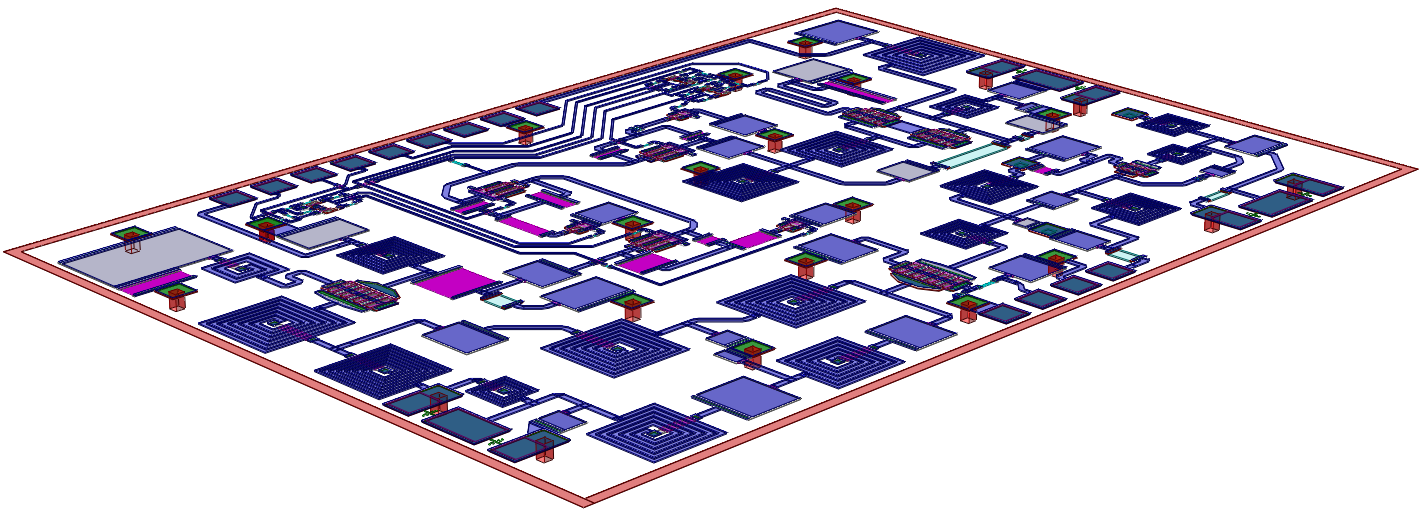
\includegraphics[width=1.0\textwidth]{fig/front_v3}

\vfill
\begin{tabular}{ll}
	Supervisors: & Niklas Billström \\
				 & Christian Fager \\
				 & \\
	Examiner:	 & Christian Fager \\
				 & Microwave Electronics Laboratory, MC2 \\
				 & Chalmers University of Technology \\
				 & Göteborg
\end{tabular}
\end{center}

\newpage	
%\clearpage
%\thispagestyle{empty}

\selectlanguage{english}
\begin{abstract}
	An S band, high-linearity down-converter is implemented using a \unit[0.25]{\mum} GaAs MMIC pHEMT-process. Using UMS' PPH25 process, an unbalanced FET resistive mixer with a lumped diplexer and an integrated square-wave LO-drive performs the down-converting. The produced narrowband IF-signal is then  amplified twice, first in an LNA and then in a highly linear amplifier. The chip has a dynamic attenuation range of \unit[10.5]{dB} and offers a maximum gain of \unit[15]{dB}. The input \unit[1]{dB}-compression point at nominal gain is \unit[10]{dBm} which estimates input $IP_3$ to \unit[20]{dBm}. The noise figure at nominal gain is \unit[11]{dB}.
	
	The chip offers down-converting of RF-frequencies between \unit[2.4 and 3.4]{GHz} for input LO-signals of \unit[-4--0]{dBm} and an image rejection of \unit[40]{dBc}. The chip size is \unit[2.9$\times$3.4]{mm}, and it is designed to fit in a \unit[4$\times$5]{mm} QFN-capsule and consumes \unit[1.0]{W} of DC power. Three control signals govern the dynamic attenuation with an LSB of \unit[1.6]{dB}.
	
	Comparative studies regarding mixer topologies and process technologies are performed. The choice of a single cold FET resistive mixer type is motivated by its linearity, small size and simplicity. A medium-power pHEMT process is chosen, as this provides improved linearity of the amplifiers as well as acceptable noise features given the requirements.

\end{abstract}

%\setcounter{page}{4}
%\newpage
\selectlanguage{swedish}
\begin{abstract}
	En linjär blandare för S-bandet har implementerats med en \unit[0.25]{\mum} GaAs MMIC pHEMT-process. För nedkonvertering används en obalanserad resistiv FET-mixer som bygger på en diplexer och en integrerad fyrkantsformad LO-signal. Den nedblandade IF-signalen förstärks två gånger, först i en lågbrusförstärkare och sedan i en effektförstärkare. Chippet har en dynamisk dämpning på \unit[10.5]{dB} och har \unit[15]{dB} maximal förstärkning. Ingångs-$P_{1dB}$ är \unit[10]{dBm}, vilket ger ett uppskattat ingångs-$IP_3$ på \unit[20]{dBm}. Vid nominell förstärkning är brusfaktorn \unit[11]{dB}.
	
Chippet klarar nedblandning av RF-frekvenser mellan \unit[2.9 och 3.4]{GHz} för LO-effekter \unit[-4--0]{dBm} och dämpning av spegelfrekvenserna med minst \unit[40]{dBc}. Chippet är designat för montering i en \unit[4$\times$5]{mm} QFN-kapsel och förbrukar \unit[1.0]{W}. Tre kontrollsignaler styr den dynamiska dämpningen med \unit[1.6]{dB} LSB.

Jämförelsestudier av blandartopologier och processval har genomförts. Blandaren är vald på grund av dess linjäritet, mindre storlek och enkelhet. UMS PPH25 process har valts då den klarar hög effekt och därmed mer linjära förstärkare såväl som acceptabla brusförhållanden givet design\-specifikationen.

	
	
\end{abstract}

\selectlanguage{english}
\newpage
\clearpage
%\thispagestyle{empty}
\section*{Preface}
	This report concludes our master's thesis work on monolithic microwave integrated circuit down-converter design. It is the degree project for our Master of Science in Engineering Physics at Chalmers University of Technology. The work has been carried out at Saab Electronic Defence Systems (former Saab Microwave) in Mölndal, Sweden, in the fall of 2010.
	
	First and foremost we would like to thank our supervisor at Saab, Niklas Billström, for his guidance during our project and for an unceasing patience. We thank our boss, Karin Adebahr, for her early faith in our abilities. We would also like to thank Simon Kristiansson, Joakim Nilsson, Peter Karlsson and the rest of the IC-design department at Saab for input during our work.
	
	Moreover, we would like to thank our supervisor and examiner at Chalmers Microwave Electronics Laboratory, Christian Fager, for his support during the project.\\[1cm]

\hfill
\begin{tabular}{ l }
Richard Abrahamsson \\
Anders Bennehag \\
Göteborg \today
\end{tabular}


	% Table of contents
	\newpage
	
	\ifdefined\saab
	\else
		\pagenumbering{roman}
		\setcounter{page}{1}
		\pagestyle{fancy}
		\setspecialhdr
	\fi
	
	%\pagestyle{fancy}
	%\setspecialhdr
	\tableofcontents
	%\newpage
	%\listoffigures
	%\newpage
	%\listoftables

	% Main body
	\newpage
	
	\ifdefined\saab
	\else
		\setdefaulthdr
		\pagenumbering{arabic}
		\setcounter{page}{1}
	\fi

	\settocdepth{section}
	\cleardoublepage
	\chapter{Introduction}
	\section{Active electronically scanned array}
		Radars of today often utilize a phased array function which permits steering of the antenna lobe by use of constructive and destructive interference. This removes the need for mechanical constructions that rotates the radar. By not having any movable parts, the reliability and performance vastly outperforms the properties of rotating radars. For example, because the angular speed of the electronically steered antenna array, the antenna lobe can simultaneously keep track of several targets while also scanning the skies for new ones. This type of radar is an electronically steered antenna, or ESA.\autocite{web:navair02}

		An ESA-antenna consists of many small antenna elements, or transmit/receive-modules. The signal's phase and amplitude are controlled individually for each TRM while other signal processing is common for groups of modules. It is therefore to one's advantage to create small antenna elements as well as small circuits controlling them. This can be done with monolithic microwave integrated circuits (or MMICs). MMICs are small, efficient and reliable, making them well-suited for radar applications.\autocite{stimson98}

		Older ESA's were usually passive (PESA); all TRMs operating at the same frequency and powered by a common source. If small groups of antenna elements are powered individually the array is active, an AESA. This gives the flexibility of being able to transmit over different frequencies at the same time and thus, amongst other things, decrease the likelihood of discovery.\autocites{oliner72}

		Common modern radars transmit at frequencies from \unit[1]{GHz} up to tens of GHz. Early digital sampling of the analogue signal enables more processing to be done in software, extending the radar's applications and utility. To perform analogue-to-digital conversion with today's technology, the frequency must be in the order of \unit[100]{MHz}. This is at least one order of magnitude less than the transmit frequencies.

		Figure \ref{fig:intro_fig} presents a usual setup of an AESA-system. The signal is received in a large number of TRM-modules where amplification and phase steering are performed. In the next step, the signal is prepared for AD-conversion by down-converting the frequency. In the third step, the signal is digitized and processed in software.

		In this thesis work, the first in a chain of necessary down-converters is designed on a GaAs MMIC. The chip is called multi-functional because it contains additional components such as amplifiers and variable attenuators. Due to the tailored performance with strict specifications and the inclusion of many components, the chip cannot be bought off the shelf. The main reason for implementing on an MMIC is the need for miniaturisation as it is important to start processing the signal as close to the antenna as possible.

		\begin{figure}[hpt!]
			\centering
			\subfloat[][]{
				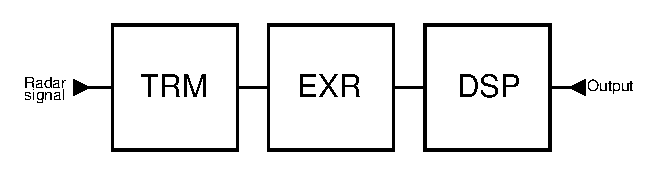
\includegraphics[width=0.7\textwidth]{fig/introduction/receiver}
				\label{fig:introreceiver}
			}\\
			\subfloat[][]{
				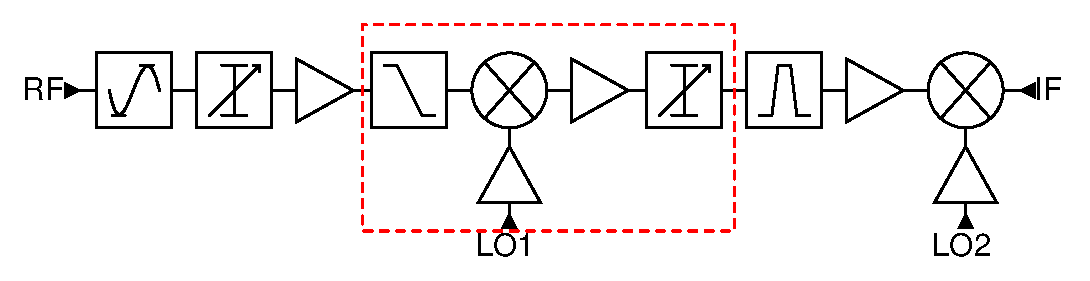
\includegraphics[width=1.0\textwidth]{fig/introduction/exr}
				\label{fig:introexr}
			}
			\caption[AESA receiver system.]{Schematic view of the AESA receiver system. \subref{fig:introreceiver} The signal is picked up by the antenna in the transmitter receiver module (TRM), processed in the exciter receiver subsystem (EXR) and finally converted to a digital signal in the DSP-unit, where digital beam forming is performed. \subref{fig:introexr} A detailed view of the EXR-unit. It contains a series of down-converters and filters. The down-converters are necessary to provide the analogue-to-digital converter with the correct frequency. This master's thesis covers the implementation of the first down-converter and a dynamic gain on an MMIC (components enclosed by a red dashed line). The chip is designed for the S band and contains image reject features. RF, LO and IF are explained in \nameref{ch:introduction_mixer} \ref{ch:introduction_mixer}.}\label{fig:intro_fig}
		\end{figure}

		%To perform analogue-to-digital conversion with today's technology, the frequency should preferably be at least one order of magnitude smaller than the carrier frequency (radio frequency or RF) of a radar which transmits/receives at \unit[3]{GHz}. In this thesis work the first in a chain of necessary down-converters will be designed on a GaAs MMIC.

	\section{Design specifics}
		As previously mentioned there is a need for a custom, very small, mixing circuit. Implementation as an integrated circuit is clearly beneficial because of the small size. In \autoref{app:specs} the full specification of the MMIC is listed. Most important are the demands on linearity, noise and gain. The gain is set to \unit[$\sim$10]{dB} with a \unit[$\pm$5]{dB} dynamic gain range. This means that the gain is variable and that the chip needs amplifiers and some means of controlling the gain. The linearity, measured using the input third-order intercept point, should be at least \unit[15]{dBm} at nominal gain. The noise figure should, for nominal gain, be less than \unit[15]{dB}. These quantities are explained later on in this chapter.


	\section{GaAs monolithic microwave integrated cir\-cuit}
		\subsection{Properties}

		MMICs offer miniaturisation of electric circuits and can be constructed with different materials having different properties. Gallium arsenide (GaAs) has been used as a semiconductor material since the 70's. When it was introduced, it was a minor revolution; the high electron mobility permitted frequencies in excess of \unit[200]{GHz} and greater breakdown voltages increased the power levels. GaAs circuits are less sensitive to heat compared to ordinary silicon semiconductor materials and offers good noise-performance.\autocite{robertson95} %page 10

		\subsection{HEMT-technology}
			The active components of MMICs are usually FETs and different processes offer different kinds of FETs.	The High Electron Mobility Transistor-, or HEMT-technology uses the quantum well created in the conduction band in the interaction between two semiconductors. The electrons in the well form a two-dimensional electron gas that can be used to form the channel region of the FET.\autocite{mimura80} The two semiconductor-materials usually must have the same lattice constants.

			Pseudomorphic HEMTs, or pHEMTs, have a very thin second layer which allows that layer to "stretch" over the first layer. This circumvents the requirement of having the same lattice constant, allowing for greater band gap difference, which gives greater power handling capabilities.

		\subsection{Foundry process}
			Foundry processes differ, both in the size of components and in the performance features, such as power capability, noise, etc. The size of a process usually refers to the gate length in its active device.

			The two processes considered for this chip are PH25 and PPH25 from UMS. United Monolithic Semiconductors (UMS) is an MMIC fabrication plant in France. Both processes utilize pHEMT-technology and have a \unit[0.25]{\mum} gate length. The difference is that PPH25 (power pHEMT) allows higher power density while PH25 has better noise performance. Another thing to consider is that UMS holds test runs for PH25 (not for PPH25) which is a cheap way of verifying a design prior to large volume orders.

			An evaluation is conducted to compare the MMIC performance for the two UMS processes. The results are found in \autoref{sec:processval} and they are based on the designs detailed in the report. From this comparison, PPH25 is chosen.

	\section{Circuit simulations}
		This project governs the design of the MMIC and does not include measurements made on an actual chip. All results documented are thus simulated results. The simulations are initially based on mathematical models of UMS' components. However, as the design matures the accuracy of these models becomes insufficient. Full electromagnetic (EM) simulations are therefore performed on all passive structures on the chip. The results in the report are all calculated using EM-simulations. More information on specifics regarding EM-simulations is found in \autoref{app:emsim}.

	\section{Mixer principles}\label{ch:introduction_mixer}
		\subsection{Mixing}

			The mixer supplies the fundamental function of down- or up-converting a signal's frequency and is principally a simple component; it receives a radio signal and together with a local oscillator an intermediate frequency is created, as seen in \autoref{fig:mixerroughschematic}. The mixer utilizes the fact that multiplication of two signals creates a signal with new frequencies

			\begin{align}\label{eq:simplemixer}
			%	\sin(|\omega_1-\omega_2| t) &= \sin(\omega_1 t)\sin(\omega_2 t) \\
				\omega_\text{IF} &= |\omega_\text{RF}\pm\omega_\text{LO}|
			\end{align}

			This is used for converting signals between different frequencies. The new signal is called the intermediate frequency and it contains the two frequencies resulting from \autoref{eq:simplemixer}. The components are called the upper and the lower sideband. There is usually a filter after the multiplication as only one of the frequency components is desired. An example is shown in \autoref{fig:mixing_function}. More details are presented in \autoref{ch:mixer}.

			\begin{figure}[hbt!]
				\centering
				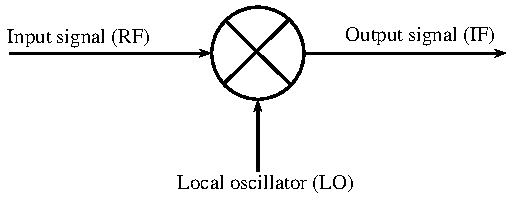
\includegraphics[width=0.6\textwidth]{fig/mixer/mixer.pdf}
				\caption{Schematic component of a mixer.}\label{fig:mixerroughschematic}
			\end{figure}

%			\begin{figure}[hbt!]
%				\centering
%				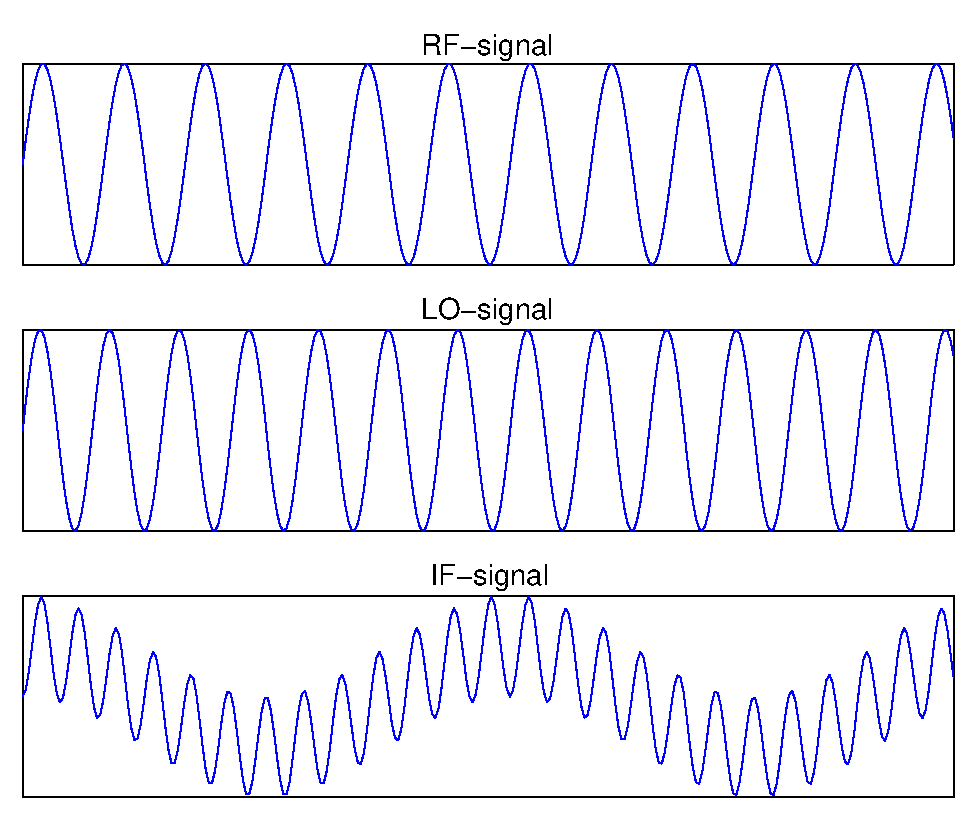
\includegraphics[width=0.6\textwidth]{fig/mixer/mixing_function}
%				\caption{}\label{fig:mixing_function}
%			\end{figure}
			\begin{figure}[hpt!]
				\centering
				\subfloat[][Time domain.]{
					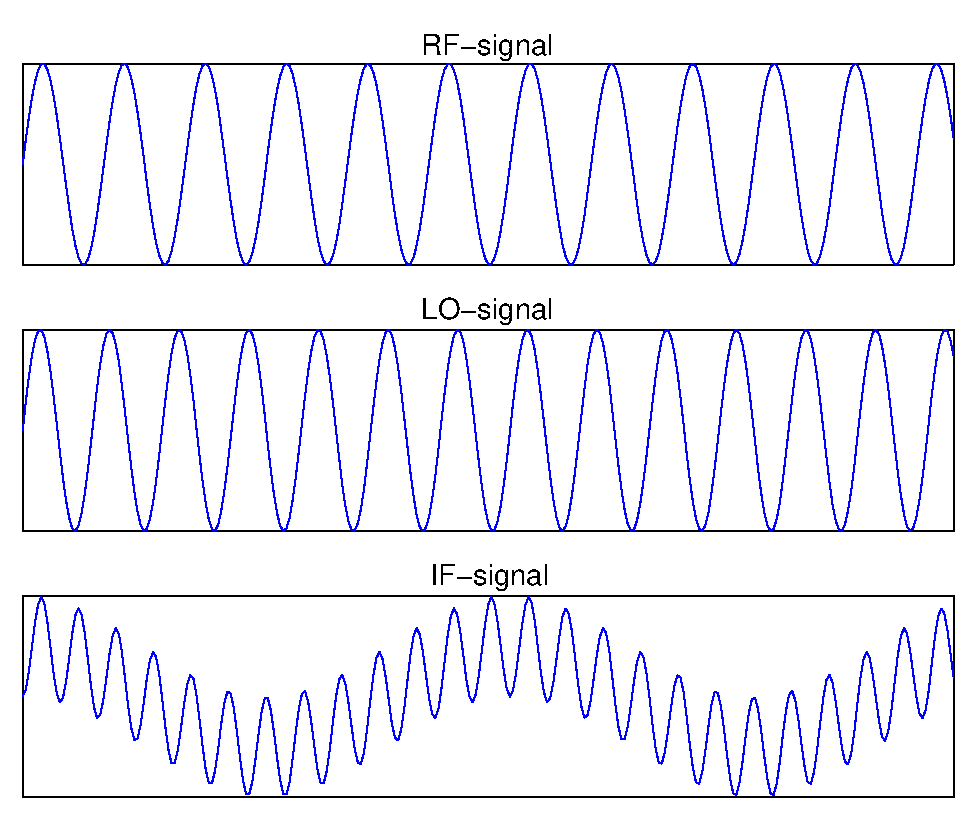
\includegraphics[width=0.5\textwidth]{fig/mixer/mixing_function}
					\label{fig:mixing_function_time}
				}
				\subfloat[][Frequency domain.]{
					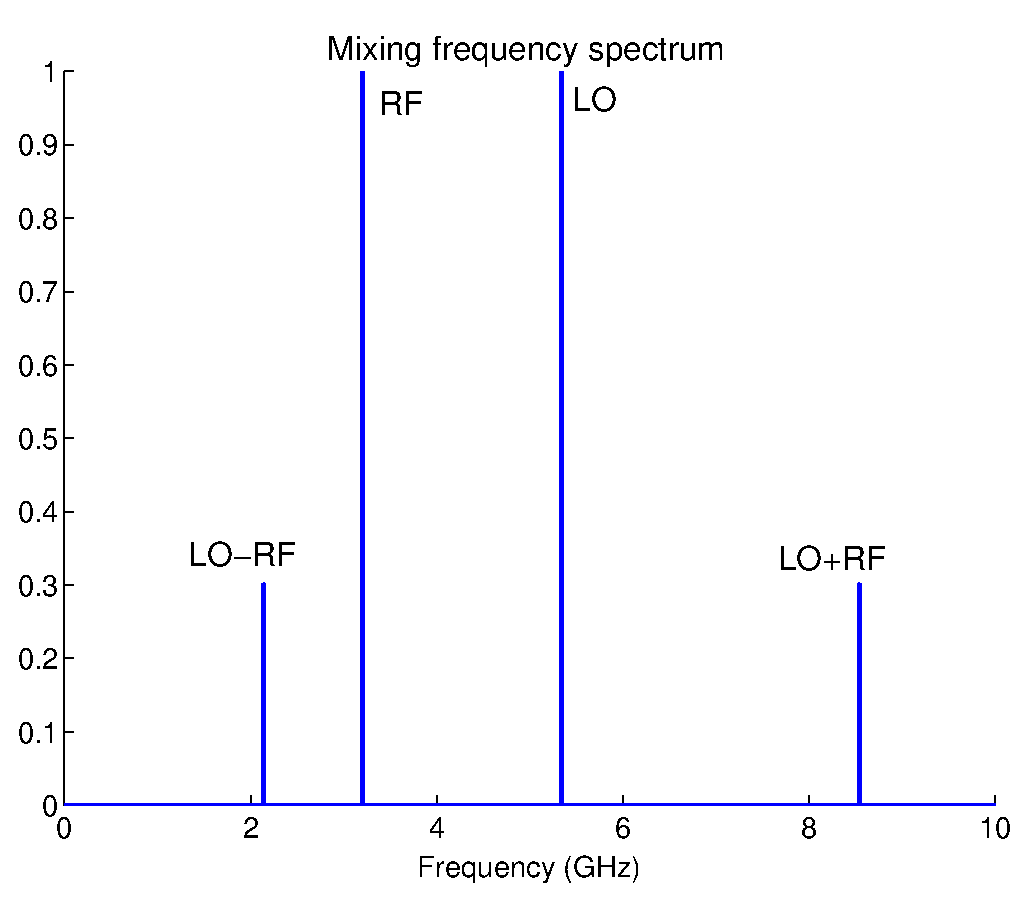
\includegraphics[width=0.5\textwidth]{fig/mixer/mixing_function_fft}
					\label{fig:mixing_function_fft}
				}
				\caption{The resulting signals from multiplication of RF- and LO-signals. The IF-signal contains both the upper and the lower sidebands.}\label{fig:mixing_function}
			\end{figure}

		\subsection{Image rejection}
			An incoming signal in the frequency band that converts to the same IF-frequency as the desired signal is called an image. Once this signal has been down-converted it becomes indistinguishable from the desired signal. To avoid this, the mixer has an image reject specification of \unit[30]{dBc}. This means that the conversion gain of the image should be at least \unit[30]{dB} lower than that of the desired band.


	\section{Intermodulation products}
		\subsection{Linearity and intermodulation}
			The operation of a mixer, or down-converter, should be as linear as possible. Linearity in the mixer ensures as few unwanted signals as possible arise from the mixing procedure. The frequencies of these spurious signals are calculated in the same manner as the down converted intermediate frequency:\autocite{bahl03}

			\begin{equation}\label{eq:spurs}
				f_{mix} = |k_1f_1\pm k_2f_2 \pm ... \pm k_nf_n|
			\end{equation}

			The order of the intermodulation products are $O=\sum_{m=1}^n|k_m|$ and the amplitude of a signal rapidly decreases as the order gets higher. The intermodulation products that are most harmful are thus low-order signals at frequencies close to the IF. The signal of interest, the IF-signal, will in a non-linear mixer become mixed up with many of these spurious signals. The source of spurious signals are not only different orders of RF and LO signal mixes but also mixes of multiple input RF signals along with the LO. Even though this creates infinite combinations of mixing frequencies, there are a few of special interest. See \citeauthor{kundert02} for a thorough theoretical treatment\autocite{kundert02}.


%			\begin{table}[hbt!]
%			\caption[Two-tone spurious signals.]{Spurious signal frequencies, within \unit[0.5]{GHz} of the IF, originating from a two-tone excitation. The frequencies are mixed according to $f_{mix} = mf_{RF1} + nf_{RF2} + pf_{LO}$ and the orders are $O=|m|+|n|$. $ f_{RF1}=\unit[3.2]{GHz}$, $ f_{RF2}=\unit[3.22]{GHz}$ and $ f_{LO}=\unit[5.34]{GHz}$.}
%			\label{tab:introtwotone}
%			\centering
%			\begin{tabular}{rrrrr}
%				m & n & p & Frequency (GHz) & Order \\\hline
%				  0 &  -6 &   4 & 2.04 & 6 \\
%				  4 &  -5 &   1 & 2.04 & 9 \\
%				 -1 &  -5 &   4 & 2.06 & 6 \\
%				  3 &  -4 &   1 & 2.06 & 7 \\
%				 -2 &  -4 &   4 & 2.08 & 6 \\
%				  2 &  -3 &   1 & 2.08 & 5 \\
%				  6 &  -2 &  -2 & 2.08 & 8 \\
%				 -3 &  -3 &   4 &  2.10 & 6 \\
%				  1 &  -2 &   1 &  2.10 & 3 \\
%				  5 &  -1 &  -2 &  2.10 & 6 \\
%				 -4 &  -2 &   4 & 2.12 & 6 \\
%				  0 &  -1 &   1 & 2.12 & 1 \\
%				  4 &   0 &  -2 & 2.12 & 4 \\
%				 -1 &   0 &   1 & 2.14 & 1 \\
%				 -5 &  -1 &   4 & 2.14 & 6 \\
%				  3 &   1 &  -2 & 2.14 & 4 \\
%				 -6 &   0 &   4 & 2.16 & 6 \\
%				 -2 &   1 &   1 & 2.16 & 3 \\
%				  2 &   2 &  -2 & 2.16 & 4 \\
%				 -3 &   2 &   1 & 2.18 & 5 \\
%				  1 &   3 &  -2 & 2.18 & 4 \\
%				 -4 &   3 &   1 &  2.20 & 7 \\
%				  0 &   4 &  -2 &  2.20 & 4 \\
%				 -5 &   4 &   1 & 2.22 & 9 \\
%				 -1 &   5 &  -2 & 2.22 & 6 \\
%				 -2 &   6 &  -2 & 2.24 & 8
%			\end{tabular}
%			\end{table}

			In order to find out which spurious frequencies are present, all low-order mixing products for the system have been calculated, using frequencies valid for the project (\autoref{tab:introsingletone}). %In the two-tone input two tones of equal amplitude, \unit[20]{MHz} apart, are fed as RF-signals.
			The order of intermodulation by convention only counts the sum of the coefficients of the RF-signals.
		
			\begin{table}[hbt!]
				\caption[Single-tone spurious signals.]{Spurious signal frequencies, within \unit[1.5]{GHz} of the IF, originating from single-tone excitation. The frequencies are mixed according to $f_{mix} = mf_{RF} + nf_{LO}$ and the orders are $O=|m|$. $ f_{RF}=\unit[3.2]{GHz}$ and $ f_{LO}=\unit[5.34]{GHz}$.}
				\label{tab:introsingletone}
				\centering
				\begin{tabular}{rrrr}
					m & n & Frequency (GHz) & Order \\\hline
	%				  4 &  -2 & 2.12 & 4 \\
	%				 -1 &   1 & 2.14 & 1 \\
	%				 -6 &   4 & 2.16 & 6 \\
					  2 &  -1 & 1.06 & 2 \\
					 -3 &   2 & 1.08 & 3 \\
					  4 &  -2 & 2.12 & 4 \\
					 -1 &   1 & 2.14 & 1 \\
					 -6 &   4 & 2.16 & 6 \\
					 -6 &  -3 & 3.18 & 6 \\
					  1 &   0 &  3.2 & 1 \\
					 -4 &   3 & 3.22 & 4
				\end{tabular}
			\end{table}

			A similar calculation of mixing products using two-tone excitation results in more spurious frequencies. The frequencies are mixed according to $f_{mix} = mf_{RF1} + nf_{RF2} + pf_{LO}$, where $f_{RF1}$ and $f_{RF2}$ are placed some tenths of MHz apart. Of special interest are the of $m$ and $n$ low odd-order signals with a low-order LO ($p=1$), and in particular the third-order intermodulation product.

		\subsection{Intercept point} \label{sec:ip3}
			Usually the third-order intermodulation products from multiple input signals cause most distortion. The third-order intercept point is an observable used to quantify the linearity in a component. Although it measures the third-order product in particular, it represents the overall linearity of a system.

			The general $n^{th}$-order intercept point, or $IP_n$, is calculated by exciting the system with two tones, as described above. The intercept point is the theoretical intercept point between the fundamental frequency and the $n^{th}$-order intermodulation product, had the gain (or loss) in the system been linear.\autocite{bahl03,pozar90} That is, for small input (system in linear region) the output of the fundamental signal increases \unit[1]{dB/dB}, and \unit[n]{dB/dB} for the $n^{th}$-order IM product. %Even though the $n^{th}$-order IM product is small for small input it will eventually grow to the same signal strength as the fundamental frequency component.
			The intercept point value is referenced either to the input power ($IIP_n$) or to the output power ($OIP_n$). The two values are determined as illustrated in \autoref{fig:introip3}.

			\begin{figure}[hbt!]
			\centering
			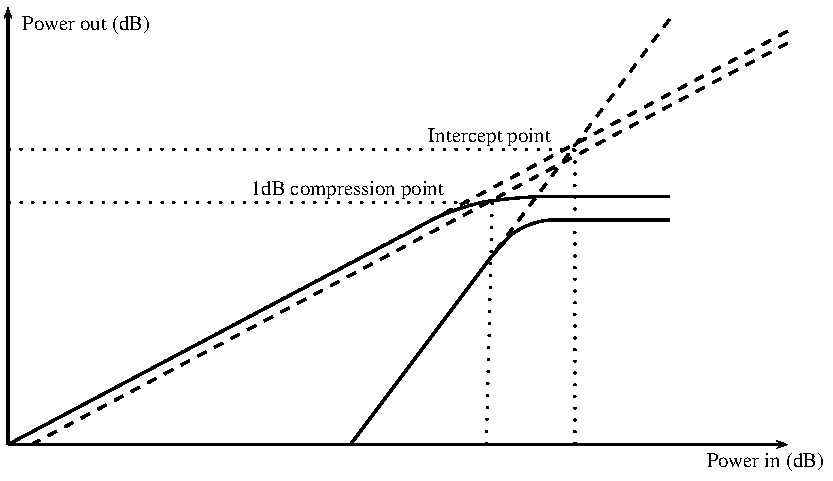
\includegraphics[width=1\textwidth]{fig/introduction/ip3.pdf}
			\caption[Definition of $n^{th}$-order intercept point and 1 dB compression point.]{The theoretical intercept point between the fundamental frequency component and an intermodulation product. The \unit[1]{dB} compression point ($P_{1dB}$) is marked as well.}\label{fig:introip3}
			\end{figure}

		\subsection{\unit[1]{dB} compression point}\label{sec:p1db}
			The \unit[1]{dB} compression point ($P_{1dB}$) is another measure of linearity. It is the point at which the output power is compressed \unit[1]{dB} compared to the linear case (\autoref{fig:introip3}). This measure is also referenced to either the input or the output power.

			$P_{1dB}$ is shown to be approximately \unit[10]{dB} lower than $IIP_3$.\autocite{kundert02} It can therefore be used as a second parameter to estimate and verify the linearity of a component in the design phase. %For the mixer component it's essential, as the simulation software is unable to apply the necessary simulation accuracy for a three-tone setup needed to calculate $IP_3$.

		\subsection{Cascaded components}\label{sec:casc_iip3}
			As circuits usually contain multiple components, such as amplifiers, mixers, filters etc, it is preferable to treat the linearity of each component individually in the design process. The total $IIP_3$ for two components is then given by \autocite{pozar90}

			\begin{equation}\label{eq:casciip3}
				I_T=\left ( \frac{1}{G_2I_1} + \frac{1}{I_2} \right )^{-1}
			\end{equation}

			$I_1$, $I_2$ and $I_T$ are the $IIP_3$ for the first component, second component and the two together, respectively. $G_2$ is the gain of the second device in the cascade. It is here evident that the order of the components is important for the total linearity.

		\subsection{Linearity simulations}
			In order to simulate a mixer's $IIP_3$ a three-tone setup is required (LO and two input RF tones). Necessary simulation accuracy for all three tones and their mixing products is very high, too high for the simulation software Microwave Office to handle. In contrast to the simpler two-tone setup required for calculating $IIP_3$ in an amplifier, the result becomes unreliable.

			The theory that results in the rule of thumb $IIP_3=P_{1dB}+\unit[10]{dBm}$ is based on a power series expansion of the transfer characteristics. A simplification to the calculations is made to only consider the first three terms. This approximation has been empirically shown to work well with amplifiers. In mixers, there is however many more harmonics present and they cannot be as easily discarded. A quick look at different papers and commercial mixers show that $IIP_3$ can be anything from \unit[6]{dBm} to \unit[14]{dBm} higher than $P_{1dB}$.

			This means that neither an estimate of $IIP_3$ from $P_{1dB}$ nor a simulation of $IIP_3$ directly are reliable methods for the mixer. The two combined gives the best hint available to a correct $IIP_3$ value.

	\section{Noise}
		\subsection{Noise sources}\label{sec:noise_thermal}
			Thermal noise arises due to collisions between electrons. As temperature increases, the particles will move faster and collide more often, thus increasing the thermal noise. The mean-square thermal noise voltage generated in a resistance $R$ over a bandwidth $\Delta f$ is\autocite{bahl03}

			\begin{equation}
				< v^2_\text{thermal} > = 4k_BTR\Delta f
			\end{equation}

			This type of noise is introduced in passive, resistive components such as resistors and inductors.

			A second type of noise present in active structures such as the FETs is shot noise. Shot noise occurs when there are not enough electrons to successfully approximate the current as continuous. The statistical variations in the electron's speed result in the sum of all electrons having variations as well. The mean-square shot noise voltage for a current $i$, in a resistance $R$, is given by
			\begin{equation}
				< v^2_\text{shot} > = 2q_eiR^2\Delta f
			\end{equation}

		\subsection{Noise in a system}
			When designing electrical circuits in general and receivers in particular, the noise must be considered at every step. Without proper design, it will be problematic to differentiate signals from the background noise. Noise has all kinds of origins; it is part of the original transmission and it is introduced while processing the signal.

			An important measure when dealing with noise is the signal to noise ratio, or SNR, which is the ratio between the useful signal and the underlying noise. It is defined as
			\begin{equation}
					\text{SNR}=20\log \left(\frac{ A_\text{signal} }{ A_\text{noise} }\right)
			\end{equation}
			where $A$ is the amplitude of the signal. In \autoref{fig:noise_example}, examples with different SNR are shown.

			\begin{figure}[hb!!!]
				\centering
				\subfloat[][]{
					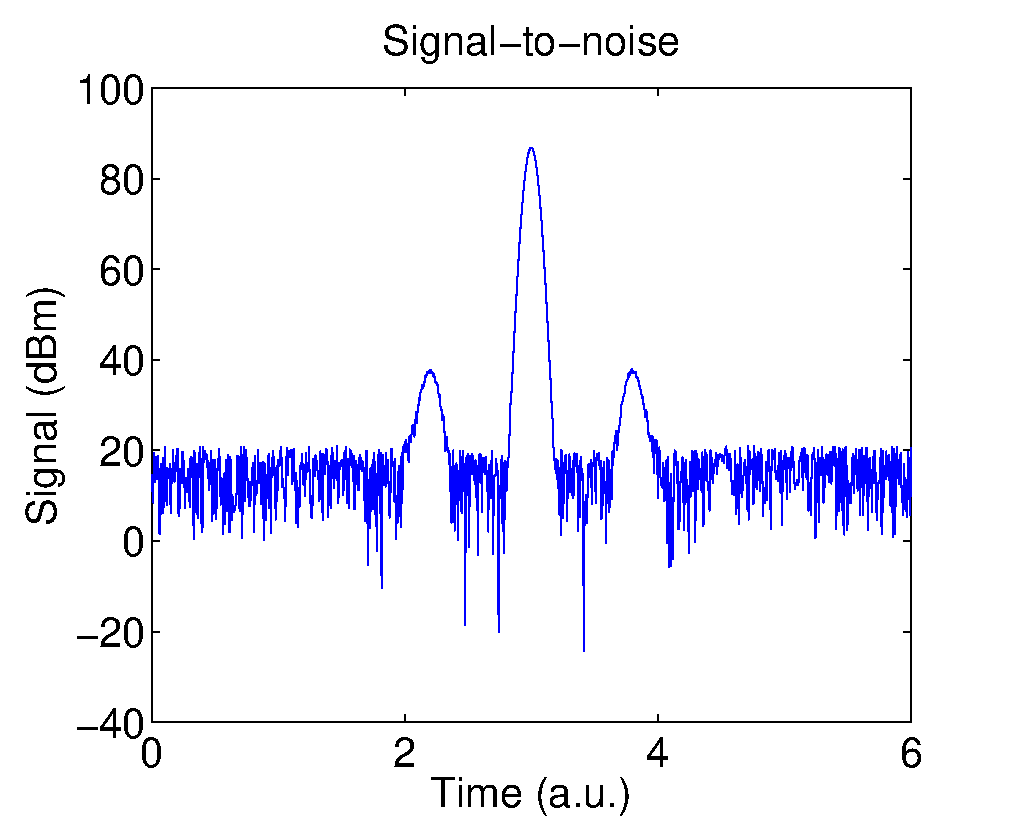
\includegraphics[width=0.5\textwidth]{fig/introduction/noise_example.eps}
					\label{fig:intro_noise_example}
				}
				\subfloat[][]{
					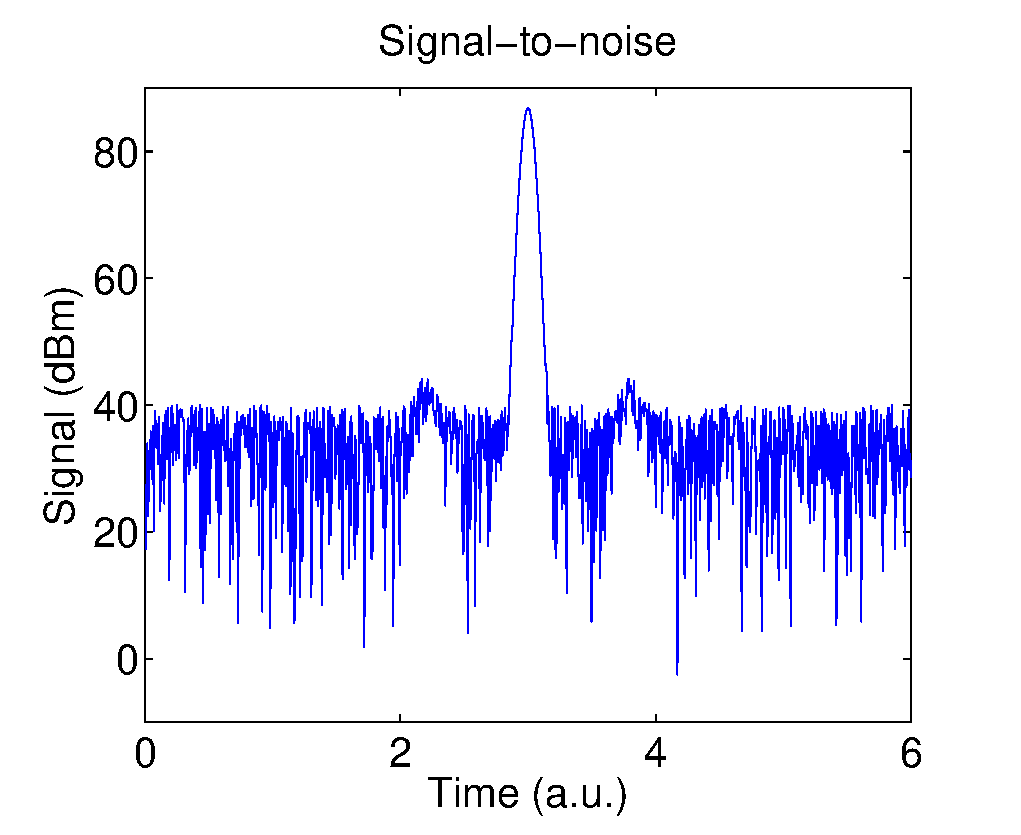
\includegraphics[width=0.5\textwidth]{fig/introduction/noise_example_2.eps}
					\label{fig:intro_noise_example_2}
				}
				\caption[Example of signal plus noise.]{\subref{fig:intro_noise_example} An example of how noise makes it difficult to measure anything but the very strong signals. The noise level and the strongest signal are found at \unit[20]{dBm} and \unit[87]{dBm}, respectively. This results in a SNR of \unit[67]{dBm}. In \subref{fig:intro_noise_example_2} the environment is noisier. The side lobes are barely visible.}\label{fig:noise_example}
			\end{figure}

		\subsection{Noise figure}
			The noise figure, or $\nf$, measures how much noise a sub circuit introduces. Introducing noise is inevitable and in order to minimize the noise, it is important to amplify the signal as early as possible and thereby raising the signal higher above the background noise. Otherwise, every subsequent attenuation of the signal will raise the noise figure just as much. $\nf$ is defined as

			\begin{equation}
				\nf=10\log \left(\frac{ \text{SNR}_\text{in} }{ \text{SNR}_\text{out} }\right) = \text{SNR}_\text{in,dB} -\text{SNR}_\text{out,dB}
			\end{equation}

			For example, in Figure\autoref{fig:intro_noise_example}, the SNR is \unit[67]{dB}. If the same ratio were to be \unit[47]{dB} after some passing through some component as in Figure\autoref{fig:intro_noise_example_2}, the noise figure for this component would be \unit[20]{dB}.


		\subsection{Cascaded components}
			The total noise figure (\nf) for a system with two components is given by \autocite{pozar90}

			\begin{equation}
				\nf_T=\nf_1+\frac{1}{G_1}(\nf_2-1)
			\end{equation}

			where $\nf_1$, $\nf_2$ and $\nf_T$ are the noise figures of the first component, the second component and the total system respectively. $G_1$ is the gain of the first component. Just as for $IIP_3$ the order of the components plays a big part of the final noise figure. In the next chapter different permutations of components are analysed for the purpose of finding which components and what order give the best trade-off between noise and linearity.

	\cleardoublepage
	\chapter{Chip Design}\label{chap:sysdes}

	The required functionality of the chip can be realized in many ways. This chapter aims at explaining and choosing an appropriate setup of sub-circuits given the requirements from SAAB.

	\section{Overall performance}
		The required performance of the down-converter is listed in \autoref{app:specs}. These specifications list requirements that the chip is expected to achieve. Besides these there is a list for targeted performance. That is, a list of important parameters of the chip that should be improved upon given the possibility. These are the bandwidth, the noise, the linearity and the power efficiency. The chip design takes all these parameters into account.

		A system's noise and linearity are counterparts. To see this dualism, a two-component system composed of a component with low attenuation and an amplifying component is considered. If the amplifier is placed before the attenuator the system's overall noise figure ($\nf$) will be only the few decibels of noise present in the amplifier. The $IIP_3$ will on the other hand be limited by the amplifier's output power. In a reversed system, with the attenuator first, the $\nf$ will become the loss in the attenuator plus the noise in the amplifier. The $IIP_3$ however, will be higher, benefiting from the initial loss according to \autoref{eq:casciip3}.

		Naturally there is a minimum of components necessary to achieve the specified performance. The mixing circuit needs a dedicated amplifier to amplify the LO-signal to an appropriate power level. Unless an image reject mixer is used, there is a need for a filter to remove the image frequencies which an opponent could use for jamming the system. The RF-to-IF chain needs amplifiers and a variable attenuator block. The nominal chip gain is set to be \unit[8--10]{dB} with a $\unit[\pm 5]{dB}$ gain control. This means that the signal must be amplified at least \unit[13]{dB} plus losses in the entire circuit. If the losses in the mixer and the attenuator block are \unit[10]{dB}, then the gain of the amplifiers must be at least \unit[23]{dB}.

	\section{Component performance}
		To estimate the performance of different layouts, typical performance of the individual components are needed. However, as this is an analysis made prior to the design, the performance is only estimated. In \autoref{tab:compperformance} the estimates are presented.

		\begin{table}[hbt!]
			\caption[Estimated performance of chip components.]{Estimated performance of the chip's components.}
			\label{tab:compperformance}
			\centering
			\begin{tabular}{ l l l l } \toprule
				& Mixer & Amplifier & Attentuators \\\midrule
				Gain & \unit[-8]{dB} & $\unit[<13]{dB}$ & \unit[-2--12]{dB} \\
				$\nf$ & \unit[8]{dB} & \unit[1--2]{dB} & \unit[2--12]{dB} \\
				$IIP_3$ & \unit[20--27]{dBm} & \unit[14--22]{dBm} & \unit[30]{dBm} \\\bottomrule
			\end{tabular}
		\end{table}

		The mixer losses are due to the two sidebands and to the reactive circuits. The inherent splitting of the signal into two sidebands effectively reduces the gain with \unit[3]{dB} (\autoref{sec:mixer_introduction}). Depending on the type of mixer, the losses in the filters and/or baluns usually amounts to about \unit[3--7]{dB}, depending on complexity. The estimates are based on the properties of resistive mixers. As explained in \autoref{sec:fet_mixers}, a resistive mixer is chosen since they are very linear. The $IIP_3$ of a mixer is the most difficult property to estimate. One of the main topics of the thesis is to evaluate the linearity of different mixer topologies. The estimate used here for mixer $IIP_3$ (\unit[25]{dBm}) as well as for losses in diplexer and mixer (\unit[8]{dB}) are therefore made in the initial mixer study reported in \autoref{ch:mixer}.

		UMS, the foundry producing the MMIC chips, have amplifiers in PPH25 with an unconditionally stable gain up to about \unit[13]{dB}, depending on the other characteristics.\autocite{pph25manual}

		Attenuator blocks from previous works have been studied and even though there are different ways to realize them, the performances are more or less the same.\autocite{gustavsson07}

	\section{Budget analysis}\label{sec:budget_analysis}
		The purpose of the budget analysis is to estimate the performance of the MMIC based on the estimates made of each individual component. With the noise target $\nf<\unit[12]{dB}$ and linearity target $IIP_3>\unit[17]{dBm}$, it is evident that the priority is high linearity and that the signal chain thus needs to start out with an attenuating device. All components placed before the mixer in the signal path need to have a \unit[0.5]{GHz} bandwidth while components placed after only need performance for a \unit[20]{MHz} narrow band. Estimates of full chip performance are made for some different component permutations at different gain states. This way, the effect on the performance due to different gain settings is taken into account.

		\begin{table}[hpt!]
			\caption[Estimated performance of chip setup 1.]{Estimated performance of chip setup 1. The order of the components is. Filter, mixer, amplifier, attenuators and amplifier.}
			\label{tab:confper1}
			\centering
			\begin{tabular}{ l l l l }
				\multicolumn{4}{c}{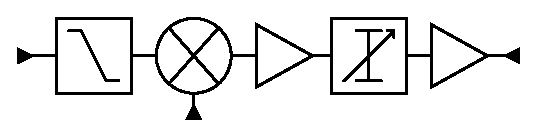
\includegraphics[width=0.6\textwidth]{fig/system/sys1}} \\\toprule
				& Nominal gain & Gain: \unit[+5]{dB} & Gain: \unit[-5]{dB} \\\midrule
				Gain & \unit[9]{dB} & \unit[14]{dB} & \unit[4]{dB} \\
				$\nf$ & \unit[10.7]{dB} & \unit[10.0]{dB} & \unit[12.4]{dB} \\
				$IIP_3$ & \unit[18.5]{dBm} & \unit[16.4]{dBm} & \unit[19.4]{dBm} \\\bottomrule
			\end{tabular}
		\end{table}

		\begin{table}[hpt!]
			\caption[Estimated performance of chip setup 2.]{Estimated performance of chip setup 2. The order of the components is: Filter, attenuators, amplifier, mixer and amplifier.}
			\label{tab:confper2}
			\centering
			\begin{tabular}{ l l l l }
				\multicolumn{4}{c}{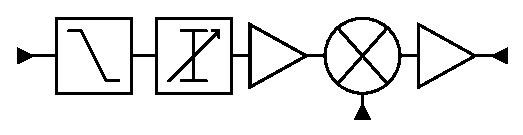
\includegraphics[width=0.6\textwidth]{fig/system/sys2}} \\\toprule
				& Nominal gain & Gain: \unit[+5]{dB} & Gain: \unit[-5]{dB} \\\midrule
				Gain & \unit[9]{dB} & \unit[14]{dB} & \unit[4]{dB} \\
				$\nf$ & \unit[12.0]{dB} & \unit[7.0]{dB} & \unit[17.0]{dB} \\
				$IIP_3$ & \unit[18.4]{dBm} & \unit[13.6]{dBm} & \unit[22.8]{dBm} \\\bottomrule
			\end{tabular}
		\end{table}

		\begin{table}[hpt!]
			\caption[Estimated performance of chip setup 3.]{Estimated performance of chip setup 3. The order of the components is: Filter, mixer, amplifier, amplifier and attenuators.}
			\label{tab:confper3}
			\centering
			\begin{tabular}{ l l l l }
				\multicolumn{4}{c}{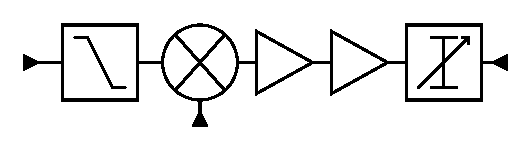
\includegraphics[width=0.6\textwidth]{fig/system/sys3}} \\\toprule
				& Nominal gain & Gain: \unit[+5]{dB} & Gain: \unit[-5]{dB} \\\midrule
				Gain & \unit[9]{dB} & \unit[14]{dB} & \unit[4]{dB} \\
				$\nf$ & \unit[9.9]{dB} & \unit[9.9]{dB} & \unit[10.1]{dB} \\
				$IIP_3$ & \unit[10.5]{dBm} & \unit[10.5]{dBm} & \unit[10.5]{dBm} \\\bottomrule
			\end{tabular}
		\end{table}

		\begin{table}[hpt!]
			\caption[Estimated performance of chip setup 4.]{Estimated performance of chip setup 4. The order of the components is: Filter, mixer, attenuators, amplifier and amplifier.}
			\label{tab:confper4}
			\centering
			\begin{tabular}{ l l l l }
				\multicolumn{4}{c}{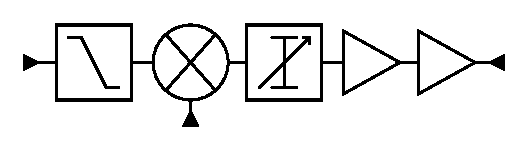
\includegraphics[width=0.6\textwidth]{fig/system/sys4}} \\\toprule
				& Nominal gain & Gain: \unit[+5]{dB} & Gain: \unit[-5]{dB} \\\midrule
				Gain & \unit[9]{dB} & \unit[14]{dB} & \unit[4]{dB} \\
				$\nf$ & \unit[16.9]{dB} & \unit[11.9]{dB} & \unit[21.9]{dB} \\
				$IIP_3$ & \unit[21.4]{dBm} & \unit[18.0]{dBm} & \unit[23.4]{dBm} \\\bottomrule
			\end{tabular}
		\end{table}

		The performance of a chip layout starting out with the gain block (\autoref{tab:confper2}) has two inherent problems. The first is that all components prior to the mixer must be wideband and the second is that the entire chip becomes very sensitive to the gain setting (compare with \autoref{tab:confper1}). Due to these, only chip layouts starting out with the mixer are considered feasible. Also, if the mixer is placed first, there are possibilities to integrate the filter with the input networks existing in most mixer designs.

		Considering the three setups starting with a mixer, the layout in \autoref{tab:confper3} gives a good noise figure but too low $IIP_3$ and the layout in \autoref{tab:confper4} gives high $IIP_3$ but too much noise. The layout in \autoref{tab:confper1}, starting out with a mixer and then alternating amplifier and attenuator, gives the best trade-off in performance and low sensitivity to different gain states. With this design, it should be possible to reach the required performance as stated in the specifications. Also the targeted performance will be met at most gain states.

	\section{Realization}
		The components are designed individually based on the above plan. Specific performance demands on individual components are discussed in depth in each section. The report is segmented to separate different classes of components such as amplifiers and mixers into different chapters.

		The mixer circuit and the image reject low-pass filter are detailed in \autoref{ch:mixer}. It starts out with a theoretical treatment of the mixing process and the importance of the LO drive. Decisions regarding topology and other design aspects follow. The design of a FET-mixer is then reported along with simulated results.

		Three different types of amplifiers are designed and reported in \autoref{ch:amp}. The first one is the LO-amplifier running in compression to provide an amplified and stable LO signal to the mixer. The second and third amplifiers are placed on the IF path, to provide the necessary chip gain. The first is designed to minimize the noise contribution while the second is designed to maximize power output and thereby chip linearity.

		Chapter \ref{ch:vargain} contains the design and results of a variable attenuator block needed to control the chip gain.

	\section{Comparison to final result}
		The figures above are based on prior estimates. \autoref{tab:confper1final} lists the results achieved with the layout in \autoref{tab:confper1} and shows a good agreement.

		\begin{table}[hpt!]
			\caption[Achieved simulated performance with chip setup 1.]{Achieved simulated performance with chip setup 1. The results are in agreement with the prior estimates detailed in \autoref{tab:confper1}.}
			\label{tab:confper1final}
			\centering
			\begin{tabular}{ l l l l }
				\multicolumn{4}{c}{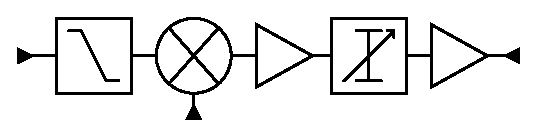
\includegraphics[width=0.6\textwidth]{fig/system/sys1}} \\\toprule
				& Nominal gain & Gain: \unit[+4.4]{dB} & Gain: \unit[-6]{dB} \\\midrule
				Gain & \unit[10.6]{dB} & \unit[15.0]{dB} & \unit[4.6]{dB} \\
				$\nf$ & \unit[11]{dB} & \unit[10]{dB} & \unit[13]{dB} \\
				$IIP_3$ & \unit[20]{dBm} & \unit[17]{dBm} & \unit[21]{dBm}  \\\bottomrule
			\end{tabular}
		\end{table}

	\cleardoublepage
	\chapter{Mixer Design}\label{ch:mixer}

	The system design chapter shows the importance of having the mixer sub-circuit first. Here we examine more in-depth how a mixer functions, different ways of realizing them, and the chosen topology in particular.

	\section{Introduction}
		\subsection{Signal multiplication}\label{sec:mixer_introduction}
			The mixer down-converts a signal by means of multiplication. The input radio frequency (RF) is multiplied with a local oscillator (LO), an external sinusoidal signal with frequency $f_{LO}$. $f_{LO}$ is selected such that one of $f_{IF}=|f_{RF}\pm f_{LO}|$ \eqref{eq:mixcos} becomes the desired down-converted signal. $f_{IF}$ is called the intermediate frequency.\autocite{maas92}

			\begin{align} \label{eq:mixcos}
				V_{RF}\cos(\omega_{RF}t)V_{LO}\cos(\omega_{LO}t)=\frac{V_{RF}V_{LO}}{2}\big[ & \cos((\omega_{RF}-\omega_{LO})t) + \nonumber \\
				& \cos((\omega_{RF}+\omega_{LO})t) \big]
			\end{align}

			The result from \autoref{eq:mixcos} requires a completely ideal multiplication device. A component with non-linear I/V-characteristics can be used for mixing, which brings about more spectral products:\autocite{bahl03}

			\begin{equation}\label{eq:poweriv}
				i = a_0 + a_1v + a_2v^2 + a_3v^3 + ... + a_Nv^N
			\end{equation}

			The current $i$ through the device depends on the sum of the two input signals $v=V_{RF}\cos(\omega_{RF}t) + V_{LO}\cos(\omega_{LO}t)$. The mixing products then become

			\begin{align}\label{eq:mixedseries}
				i = a_0 &+ a_1\left[ V_{RF}\cos(\omega_{RF}t) + V_{LO}\cos(\omega_{LO}t) \right] \nonumber \\
				& + a_2\left[ V_{RF}\cos(\omega_{RF}t) + V_{LO}\cos(\omega_{LO}t) \right]^2 + ... \nonumber \\
				& + a_N\left[ V_{RF}\cos(\omega_{RF}t) + V_{LO}\cos(\omega_{LO}t) \right]^N
			\end{align}

			The output current $i=i_{DC}+i_{IN}+i_{SPUR}$ contains a DC current term ($i_{DC} = a_0 + a_2(V_{RF}^2+V_{LO}^2)+...$), the original signals ($i_{IN}=a_1(V_{RF}\cos(\omega_{RF}t) + V_{LO}\cos(\omega_{LO}t))$) and the mixing products ($i_{SPUR}$). The second-order terms are the primary mixing products and contains the upper ($\omega_{RF}+\omega_{LO}$) and the lower ($\omega_{RF}-\omega_{LO}$) sidebands:

			\begin{align}\label{eq:mixedsecondorder}
				i_{2nd} = &a_2 \left [ \frac{1}{2}V^2_{RF}(1-\cos(2\omega_{RF}t)) + V_{RF}V_{LO}(\cos((\omega_{RF}-\omega_{LO})t) \right. \nonumber \\
				&\left. + \cos((\omega_{RF}+\omega_{LO})t)) + \frac{1}{2}V^2_{LO}(1-\cos(2\omega_{LO}t)) \right]
			\end{align}

			In this design the lower sideband is the desired intermediate frequency $\omega_{IF}$.

		\subsection{LO drive}\label{sec:mixer_lodrive}
			Regardless of topology and design choice, all mixers need an LO reference signal. This signal, or drive, is usually very large in comparison to the RF and IF signals in order to increase mixer linearity. A large LO drive will, from the RF signal's point of view, switch the mixer between on- and off-states faster, making the multiplication of the signals digital. The larger the LO drive the faster the transition between on and off states takes place. This results in more linear operation.\autocite{maas92}

			For the $P_{1dB}$ measure, not only fast on- and off-transitions are important but also the power of the LO. As explained in \autoref{sec:p1db} $P_{1dB}$ is simulated by noting at which power the gain of a component has dropped \unit[1]{dB}. When the power of the RF-signal becomes the same order of magnitude as the power of the LO drive, the LO-signal will no longer be able to switch the mixing-FET as desired. This will cause the gain to drop and thus limit $P_{1dB}$. As $IIP_3$ is closely coupled to $P_{1dB}$, this will also be limited.\autocite{kundert02}

	\section{Topologies}
		\subsection{Overview}
			The mixing functionality can be realized with a number of different mixing devices and different balanced or unbalanced designs. The literature presents two preferred devices used to multiply two signals; the diode and the transistor.\autocite{norman2002design}

		\subsection{Balanced and unbalanced mixers}
			An ordinary unbalanced mixer exhibits the behaviour where all spurious products from \autoref{eq:spurs} are present. By utilizing a balanced layout with two or more mixing elements, it is possible to suppress some of these spurious responses. There are many kinds of balanced mixers and the type determines what spurious responses are suppressed.\autocites{maas92}{dinari09}

			The downside is that additional elements must be introduced in the form of hybrids or baluns and these are often relatively large on MMICs, depending on frequency. These elements either phase shift or convert the signal between balanced and unbalanced signals.

		\subsection{Image reject mixers}
			Two mixers can be designed as an image reject mixer which cancels out the image frequency. That is the frequency that converts to the exact same IF-signal as the RF and is almost always an unwanted product. See \autoref{sec:mixer_introduction}.

			The image reject functionality is achieved, in short, when the LSB and USB (lower and upper sideband respectively) are subjected to different phase shifts in the hybrids. This makes it possible to cancel out or suppress one of the sidebands depending on the quality of the hybrids and mixers. The image reject performance is very dependant on the precision of the baluns, more specifically the degrees of phase-shift and amplitude difference.\autocite{henderson85} %Finns en artikel som visar exact vilken undertryckning man får för olika baluner

			These constructions are most useful in situations when the image band lies close to the IF. In this case the IF-signal has the frequency \unit[2.14]{GHz} and the image band starts at \unit[7.18]{GHz}. With this large distance in frequency the image is easily filtered and an image reject topology is therefore not considered.

		\subsection{Diode mixers}
			Diode mixers are realized with Schottky diodes because of their switching speed. Today diode mixers are more prevalent for high frequencies, where FETs are less potent. An advantage with diode mixers is that they do not need a bias voltage.

		\subsection{FET mixers}\label{sec:fet_mixers}
			FET mixers generally have lower noise and higher gain compared to diode mixers. There are in general two approaches to designing a FET-mixer; active or resistive mixer. MMIC processes are optimized for FET-structures, not diodes. A major advantage with FET-mixers is the inherent isolation between the LO and the IF provided by the FET.

			Active FET mixers are biased like an amplifying element and thus have a positive conversion gain while resistive mixers are biased with zero $v_{ds}$ and $v_{gs}$ below pinch-off such that the drain-source resistance is linear to the applied gate-voltage. When considering linearity, resisistive mixers are superior.\autocites{maas92,maas98}

		\subsection{Conclusion}
			Almost all MMIC mixers designed for the S band are today FET mixers. Diodes are common only when designing mixers with frequencies at least one order of magnitude higher or using discrete components. Since high linearity is important, a FET resistive mixer is designed. To decide whether to implement it as single-ended or as singly balanced, both types are initially designed with simple ideal components. The single-balanced mixer is eventually disregarded due to its complexity and to the fact that the single-ended mixer shows adequate performance. The comparison is detailed in \autoref{sec:endvsbal}.

	\section{Design of single-ended FET resistive mixer}
		\subsection{Device}\label{sec:mixerdevice}
			As described in \autoref{sec:mixerbias} higher LO power will result in a more linear mixer. The greater the gate width, the more LO power the FET can handle. The largest FET in the UMS process has a \unit[8$\times$75]{\mum} gate width. As it turns out, this is also the FET which gate is easiest to match to $\unit[50]{\Omega}$.\autocite{gustavsson07}

			 A shunt inductance is placed at the gate to the mixing FET in order to ensure that the FET bias point remains fixed at high LO power. The inductance is part of the matching network in the LO-amplifier.

		\subsection{Diplexer}
			The overall simplicity of the FET resistive mixer makes the diplexer the most sophisticated part and also crucial to the performance (\autoref{fig:mixerDiplexer}). Between the RF input and the mixer FET, the network has to band-pass filter the signal in order to both inhibit the IF-signal from leaking out and to suppress the radar image at $f_{image}=f_{LO}+f_{IF}$. Once the image frequency has passed this filter it will mix down to $f_{IF}$ and from there be indistinguishable from the original signal:

			\begin{equation}
				|f_{image}\pm f_{LO}| = |f_{LO}+f_{IF}\pm f_{LO}| = \left \{
				\begin{array}{ll}
					2f_{LO}+f_{IF}, & \text{Easily filtered} \\
					f_{IF},	& \text{Harmful}
				\end{array}
				\right.
			\end{equation}

			\begin{figure}[hbt!]
				\centering
				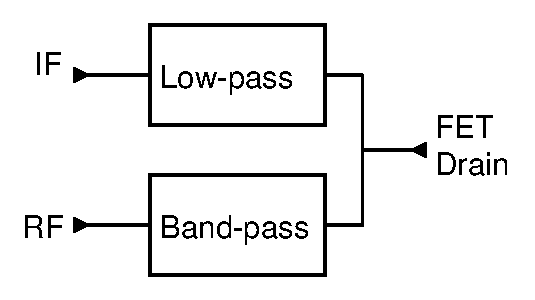
\includegraphics[width=0.5\textwidth]{fig/mixer/diplexer}
				\caption[Mixer diplexer signal path]{This diplexer consists of a low-pass filter and a band-pass filter. The signal is band-pass filtered, mixed at the FET and then low-pass filtered. Both filters are designed to match the signal to the port at the appropriate frequencies.}\label{fig:mixerDiplexer}
			\end{figure}

			Between the mixer FET and the IF output, the diplexer must low-pass filter to reject any signals above the down-mixed lower sideband frequency at $f_{IF}$. Additional filtering is done in the subsequent amplifiers.

			Besides  filtering, the diplexer has to match  both the input signal and the output signal. The input RF port is matched to \unit[50]{$\Omega$} at $\unit[2.9-3.4]{GHz}$ and the output IF port is matched to \unit[50]{$\Omega$} at \unit[2.14]{GHz}.

			The diplexer is implemented using non-resistive L-C circuits with the number of poles required to fulfil the chip specifications. The losses in the inductors add directly to the overall noise figure of the chip. The result is therefore a trade-off between filter characteristics and network simplicity.

		\subsection{Bias scheme}\label{sec:mixerbias}
			The principle of the mixer is to set the gate-source voltage $v_{gs}$ below pinch-off and then control the FET with the LO-signal. Pinch-off for the FET is $v_p\approx \unit[-0.7]{V}$. A low distortion mixer is achieved by having high LO power and thereby reducing the rise-time when the FET switches on and off. This way less time is spent operating in regions where $v_{gs}$ is close to $v_p$ (operation at gate voltages close to $v_p$ are more non-linear). However, an LO powered too high will cause the gate to rectify and this will in turn lead to non-linear operation.\autocite{maas98} By lowering $v_{gs}$ even more below $v_p$ this can be avoided. The gate will also start to break down for too large negative gate voltages, providing a lower limit for $v_{gs}$.

			As the chip is fed a $+\unit[5]{V}$ DC, the source and drain are both raised to $|v_{gs}|$ for the mixer to experience an effective negative gate voltage and $v_{ds}=\unit[0]{V}$. The bias network is placed at the source and two large value resistors divide the voltage appropriately. No DC-current will pass through the resistors.

	\section{Schematics and layout}
		The schematic of the final resistive FET mixer is shown in \autoref{fig:mixerschematic}. The corresponding layout is found in \autoref{fig:mixerlayout}.

		\begin{figure}[hbt!]
			\centering
			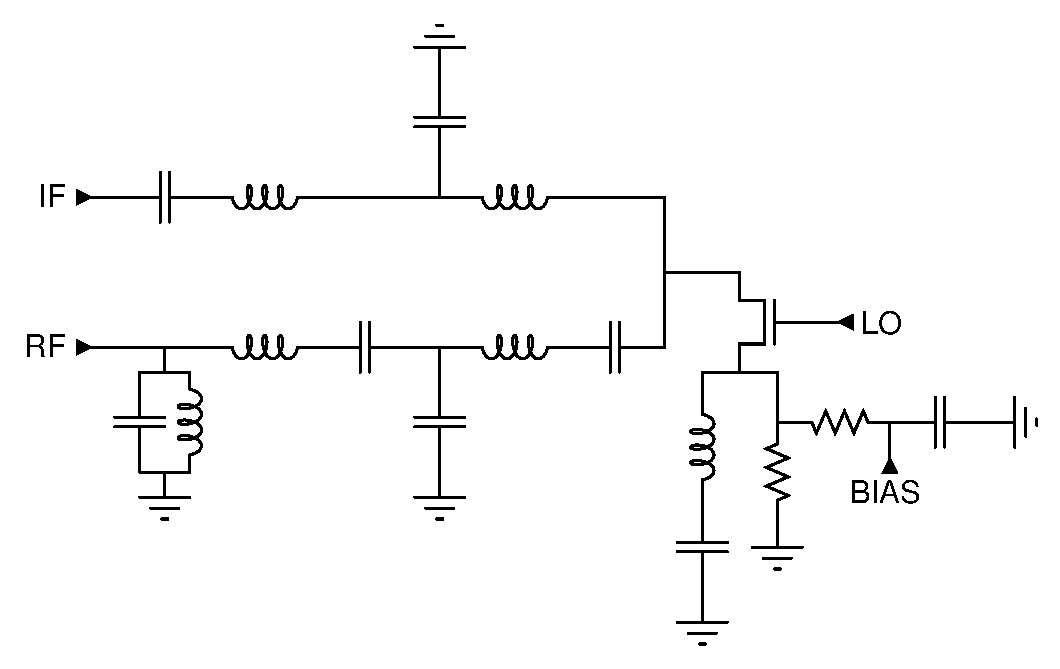
\includegraphics[width=1.0\textwidth]{fig/mixer/sch_mixer}
			\caption[Mixer schematic.]{Schematic of the mixer.}\label{fig:mixerschematic}
		\end{figure}

		\begin{figure}[hbt!]
			\centering
			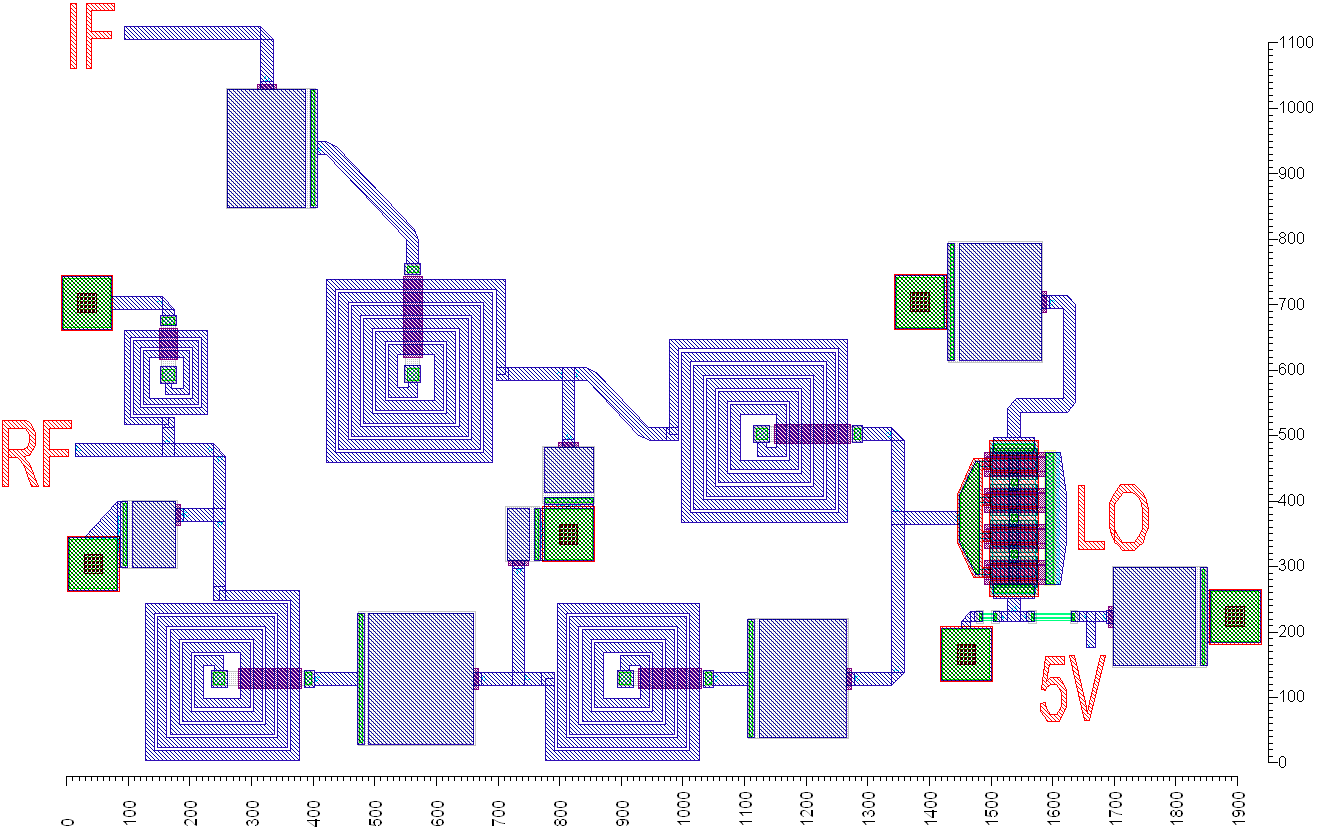
\includegraphics[width=1.0\textwidth]{fig/mixer/layout}
			\caption[Mixer layout.]{Layout of mixer.\scalemum}\label{fig:mixerlayout}
		\end{figure}

	\section{Simulation results}\label{sec:mixer}
		\subsection{Overview}
			A summary of the mixer's performance is listed in \autoref{tab:resultmixer}. Simulations are made using the LO-amplifier to provide the LO-signal. This amplifier is explained in \autoref{sec:lo_amp} but knowing it amplifies the system's LO-signal is enough to understand this mixer-chapter. All sub-circuits apart from the FETs are simulated with EM-models, see \autoref{app:emsim} for an explanation of the EM-simulations. Yield simulations are found in \autoref{sec:yield_analysis}.

			\begin{table}[hbt!]
				\caption[Simulation result of the mixer.]{Simulation results of the mixer for $LO=\unit[-2]{dBm}$ and $v_{gs}=\unit[-0.95]{V}$.\disclaimer}
				\label{tab:resultmixer}
				\centering
				\begin{tabular}{ l c c c c c c l } \toprule
					Parameter & Min. & Typ. & Max. & Min. & Typ. & Max. & Unit \\\midrule
					Frequency range RF & \multicolumn{3}{c}{2.9--3.4} & \multicolumn{3}{c}{3.1--3.3} & GHz \\
					Frequency range LO & \multicolumn{3}{c}{5.04--5.54} & \multicolumn{3}{c}{5.24--5.44} & GHz \\
					Frequency IF & \multicolumn{3}{c}{2.14} & \multicolumn{3}{c}{2.14} & GHz \\
					Return loss RF & 14 & 16 &  & 20 & 21 &  & dB \\
					Return loss Out & & 16 & & & 16 & & dB \\
					Conversion loss &  & 7.7 & 7.9 &  & 7.5 & 7.6 & dB \\
					Gain Variation & & 0.45 & 0.45 & & 0.05 & 0.05 & dB \\
					Image Rejection & 48 & 50 &  & 50 & 51 &  &  dB \\
					$P_{1dB}$ (input) & 12.7 & 13 &  & 12.7 & 13 &  & dBm \\
					$IIP_3$ (estimate) & 23 & 23 &  & 23 & 23 &  & dBm \\
					Noise figure &  & 7.7 & 7.9 &  & 7.5 & 7.6 & dB \\\bottomrule
				\end{tabular}
			\end{table}

		\subsection{Filter characteristics}
			The most important part of the diplexer filter characteristics is shown in \autoref{fig:diplexer_results}. The figure shows the EM simulated diplexer as well as a spread analysis made on the circuit model. How the spread analysis is performed is explained in-depth in \autoref{sec:yield_analysis}. For the full \unit[0--10]{GHz} frequency characteristics see Figure\autoref{fig:yielddiplexer}.

			\begin{figure}[hbt!]
				\centering
				\includerect{1.0\textwidth}{fig/yield/diplexer_zoom}
				\caption[Diplexer filter characteristics.]{Diplexer filter characteristics. The red (thick) line is the EM simulation and the blue lines correspond to the spread analysed with the circuit model. The curves marked with triangles $\triangle$ details the bandpass filter between the RF input and the mixer-FET drain. The curves marked with squares $\medsquare$ details the low-pass filter between the mixer-FET drain and the IF output.}\label{fig:diplexer_results}
			\end{figure}

		\subsection{Conversion gain and matching}
			Mixer gain (\autoref{fig:mixergain}) and input matching (\autoref{fig:mixermatch}) are calculated with the final LO-amplifier connected and using large signal analysis. The bias point does not effect neither the conversion gain nor the input matching much. The matching of the RF-port is quite independent of the LO power. The gain depends on the LO-signal which in turn depends on the LO input power. Different settings on the chip's gain block located after the first IF amplifier does not to affect the performance of the mixing part, which is why simulations with varied chip gain are not displayed. The final bias point is chosen to $v_g=\unit[-0.95]{V}$.

			\begin{figure}[hpt!]
				\centering
				\subfloat[][Conversion gain for different LO powers at $v_{gs}$=-0.95 V.]{
					\includerect{0.5\textwidth}{fig/mixer/convgainvslo}
					\label{fig:mixergainvslo}
				}
				\subfloat[][Conversion gain for different bias points $v_{gs}$ between -1.05 V and -0.75 V at $LO$=-2 dBm.]{
					\includerect{0.5\textwidth}{fig/mixer/convgainvsbias}
					\label{fig:mixergainvsbias}
				}
				\caption[Mixer conversion gain.]{Mixer conversion gain.}\label{fig:mixergain}
			\end{figure}

			\begin{figure}[hpt!]
				\centering
				\subfloat[][Input matching for different LO powers at $v_{gs}$=-0.95 V..]{
					\includerect{0.5\textwidth}{fig/mixer/matchvslo}
					\label{fig:mixermatchvslo}
				}
				\subfloat[][Input matching for different bias points $v_{gs}$ between -1.05 V and -0.75 V at $LO$=-2 dBm.]{
					\includerect{0.5\textwidth}{fig/mixer/matchvsbias}
					\label{fig:mixermatchvsbias}
				}
				\caption[Mixer RF-input matching.]{Mixer RF-input matching.}\label{fig:mixermatch}
			\end{figure}

		\subsection{Linearity}
			\autoref{fig:mixerp1dbvsbias} illustrates the compression of the conversion gain for different bias points $v_{gs}$. $P_{1dB}$ is the point where the conversion gain has dropped \unit[1]{dB} and is usually referenced to the input power. $P_{1dB}$ as a function of frequency and LO input power are plotted in \autoref{fig:mixerp1db}.

			\begin{figure}[hbt!]
				\centering
				\includerect{0.7\textwidth}{fig/mixer/p1dbvsbias}
				\caption[Mixer conversion gain compression.]{Mixer conversion gain compression for different bias points $v_{gs}$. Here $LO=\unit[-2]{dBm}$ and $f=\unit[3.2]{GHz}$. The compression does not vary with the bias point.}\label{fig:mixerp1dbvsbias}
			\end{figure}

			\begin{figure}[hpt!]
				\centering
				\subfloat[][$P_{1dB}$ versus frequency for $LO$=-2 dBm and $v_{gs}$=-0.95 V.]{
					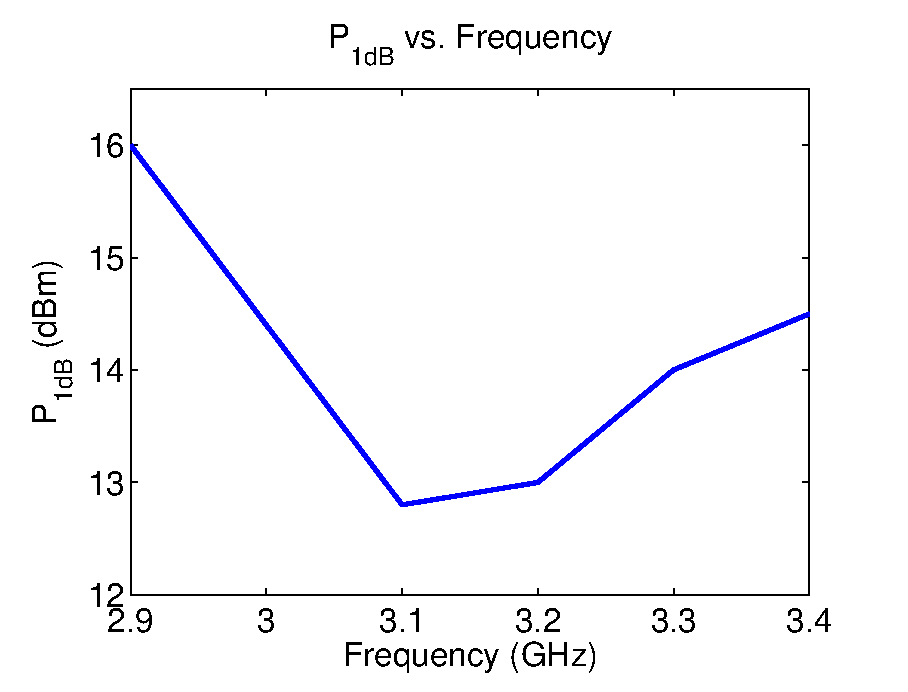
\includegraphics[width=0.5\textwidth]{fig/mixer/p1dbvsfreq}
					\label{fig:mixerp1dbvsfreq}
				}
				\subfloat[][$P_{1dB}$ versus LO power for $f$=3.2 GHz and $v_{gs}$=-0.95 V.]{
					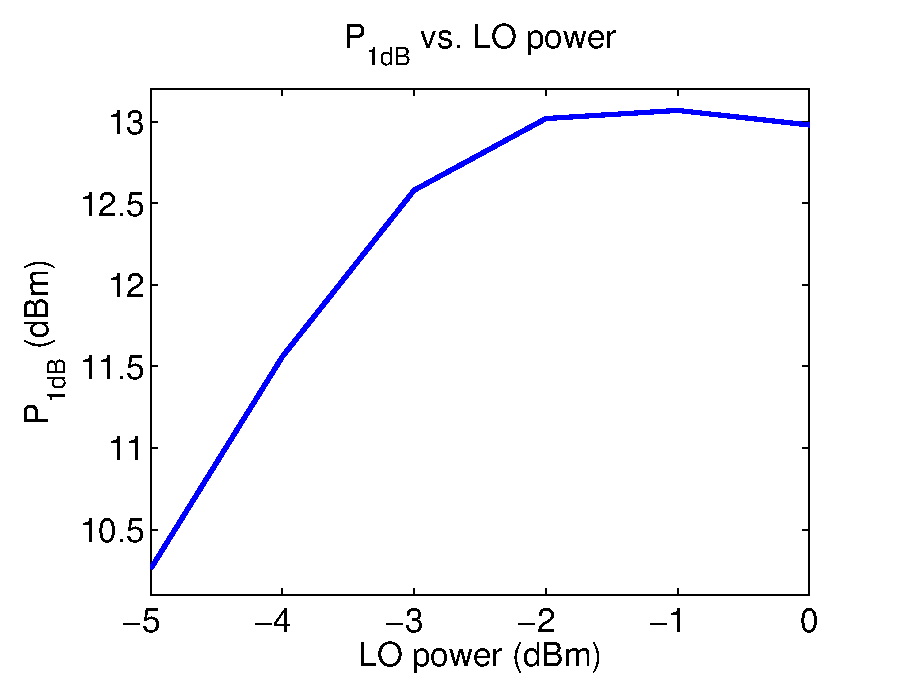
\includegraphics[width=0.5\textwidth]{fig/mixer/p1dbvslo}
					\label{fig:mixerp1dbvslo}
				}
				\caption[Mixer $P_{1dB}$.]{Mixer $P_{1dB}$ versus frequency and LO power.}\label{fig:mixerp1db}
			\end{figure}

		\subsection{Image reject}
			The conversion gain of the RF image at $f_{LO}+f_{IF}=$\unit[7.18--7.68]{GHz} is displayed in \autoref{fig:mixerimr}.

			\begin{figure}[hbt!]
				\centering
				\includerect{0.7\textwidth}{fig/mixer/imr}
				\caption[RF-image conversion gain.]{Conversion gain with the RF-image as the input signal.}\label{fig:mixerimr}
			\end{figure}

	\section{Discussion}
		As discussed in the performed topology study there a few sophisticated designs that may give very good mixer performance. The achieved performance and the simple design of the single-ended resistive FET mixer is however undeniable. Not only does this save design effort but also space on the chip and thereby also money in yield and wafer costs. It is not surprising that the industry in general chooses this topology for high linearity mixers at these frequencies.\autocite{web:hittite}

		The noise figure in the mixer is casually considered equal to the losses. Even though this is a popular approach there are some ways to take noise generated in the mixer into account.\autocite{kundert07} However, since the noise figure is generally somewhat lower than the losses, the conversion loss is taken as a high estimate of the noise, disregarding the more accurate noise calculations.

		Low accuracy three-tone $IIP_3$ simulations yield a result \unit[2--3]{dBm} higher than the estimates made from $P_{1dB}$. Due to their uncertainty, these results are not reported here and are only mentioned in this discussion for reference.

	\cleardoublepage
	\chapter{Amplifier Design}\label{ch:amp}

	After down-conversion, the signal must be amplified twice according to the chip design in \autoref{chap:sysdes}. Furthermore, the LO-signal controlling the mixer also needs amplification. The function and purpose of these three amplifiers are explained in this chapter.

	\section{Introduction}
		\subsection{Function}
			The purpose of an amplifier is to amplify electric signals. In a radar receiver setup the amplifier is often, after a limiter and a filter, the first element an incoming signal sees. Any degradation of the signal's power before the first amplification increases the noise (see \autoref{fig:noise_example}). The main goal of such an amplifier is to provide gain without adding noise and is called an LNA (low noise amplifier).

			The last amplifier in a transmitter-setup is more focused on providing as much gain and output power as possible without consuming too much power. For most amplifiers it is also of concern to operate linearly. This is measured with $IIP3$ and $P_{1dB}$ as explained in \autoref{sec:ip3}.

			An amplifier designed with FET-technology needs a drain-supply voltage $v_{ds}$ (drain-source), see \autoref{fig:fet-illustrative}. The current through the FET, $i_{ds}$ (drain-source current), depends on the gate-source voltage $v_{gs}$ which, in effect, is the incoming signal fed to the gate-terminal. It is the time-varying $i_{ds}$ that creates the amplification.

		\begin{figure}[hbt!]
			\centering
			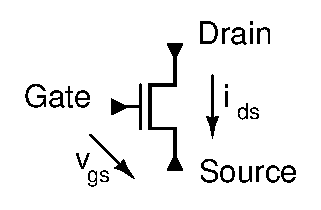
\includegraphics[width=0.3\textwidth]{fig/amplifiers/fet-illustrative}
			\caption[The ports of a FET.]{The ports of a FET. The voltage $v_{gs}$ (gate-source) controls how much current $i_{ds}$ can flow through the FET.}\label{fig:fet-illustrative}
		\end{figure}

		\subsection{Bias point}
			When operating the FET, there are in general four different bias points corresponding to different classes of amplifiers.\autocite{gonzalez84} These are seen in \autoref{fig:fet_bias_point}. For low noise operation, bias point A is common and for high output-power and class A operation, bias point C is more prevalent.

			\begin{figure}[hbt!]
				\centering
				\includegraphics[width=0.5\textwidth]{fig/amplifiers/fet_bias_point}
				\caption{Different bias points for a FET.}\label{fig:fet_bias_point}
			\end{figure}

		\subsection{Bias scheme}\label{sec:bias}
			The amplifiers in this project are biased using the self-biasing scheme in \autoref{fig:if1bias}.\autocite{bahl03} This limits the size and complexity of the bias network as only one (positive) DC source is supplied. The PPH25 process can, contrary to PH25,  handle a higher drain-source voltage $v_{ds}$ over the FET. This further simplifies the biasing as the supplied \unit[5]{V} DC voltage can be applied without the need of a resistor on the drain, given that this constitutes an appropriate bias point.

			\begin{figure}[hbt!]
				\centering
				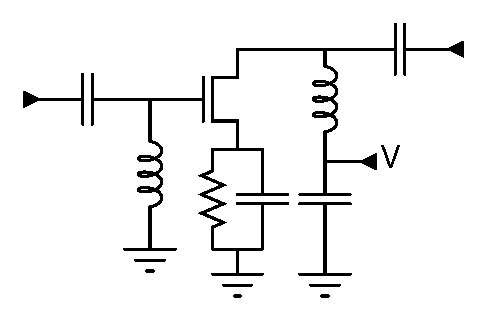
\includegraphics[width=0.5\textwidth]{fig/amplifiers/if1/bias}
				\caption[Self-bias scheme.]{The principle of the self-biasing scheme. The FET's drain is raised to \unit[5]{V} and the gate is DC-grounded. The resistor on the source controls the bias voltage $v_{gs}$ and thereby also the bias-current $i_{ds}$.}\label{fig:if1bias}
			\end{figure}

		\subsection{Stability}
			A stable amplifier ensures that there is no oscillation.\autocite{grosch99} The amplifiers on this chip are all designed to be unconditionally stable at all frequencies. Generally, an amplifier with higher gain is harder to make stable. The stability measure $K$ in \autoref{eq:kstability} is used to quantify stability. An amplifier is unconditionally stable if $K>1$ for all frequencies.

			\begin{equation}\label{eq:kstability}
				K=\frac{1+|S_{11}S_{22}-S_{12}S_{21}|^2-|S_{11}|^2-|S_{22}|^2}{2|S_{12}||S_{21}|}
			\end{equation}

		\subsection{Power utilization}\label{sec:power}
			As the DC-power consumption of an amplifier increases, the linearity ($P_{1dB}$ and $IIP_3$) increases. This is evident as compression will occur at higher power (\autoref{sec:p1db}). The LO amplifier is designed to operate in compression and as such it does not benefit from high power. The remaining available DC-power is divided between the first and the second IF amplifier. As the $IIP_3$ for the second amplifier affects the chip more than that of the first one, the power utility here is higher.

	\section{Constant power LO-amplifier}\label{sec:lo_amp}
		\subsection{Introduction}
			The input LO-signal is specified to \unit[-5--0]{dBm} and there is therefore a need to amplify this signal. The purpose of the amplifier is to provide a high and constant input power to the mixer, not sensitive to fluctuations of the input LO-signal. This is achieved by operating the amplifier in compression so that the mixer always sees the same LO. Also, by running the amplifier in compression, i.e. outputting a square-waved pulse, the mixer will switch faster between the on- and off-states, behaving more like an ideal switch. This results in a more linear mixer as explained in \autoref{sec:mixer_lodrive}.\autocite{vice03} %The LO-amplifier is matched against the mixer which is a highly reactive load.



		\subsection{Design}
			\subsubsection{Principle}
				When designing an LO-amplifier for a resistive FET mixer, it is important to minimize reflections from the very reactive mixer-gate. However, attaining a well-matched gate is difficult.\autocite{yhland1999} At first, a bias-point is chosen, such that proper gain and compression is achieved. As a \unit[0.5]{GHz} bandwidth is important, a weak feedback loop ($\unit[500]{\Omega}$) is used. A too strong feedback is undesirable because of the reduced gain and stability. The FET is self-biased by applying a voltage to the drain, while having $v_{DC}=\unit[0]{V}$ on the gate (see \ref{sec:bias} \nameref{sec:bias}). This requires having an inductance to ground close to the gate. Schematic and layout of the amplifier are seen in \autoref{fig:sch_lo} and \autoref{fig:lo_layout}, respectively.



				As noise is not of much concern for the LO, it can be traded for stability, compression, ease of tuning and frequency independence. Since linearity is actually to be avoided and the amplifier never enters high-linearity bias-regions such as for class A-operation, the amplifier consumes small amounts of power, around \unit[100]{mW}.




			\begin{figure}[hbt!]
				\centering
				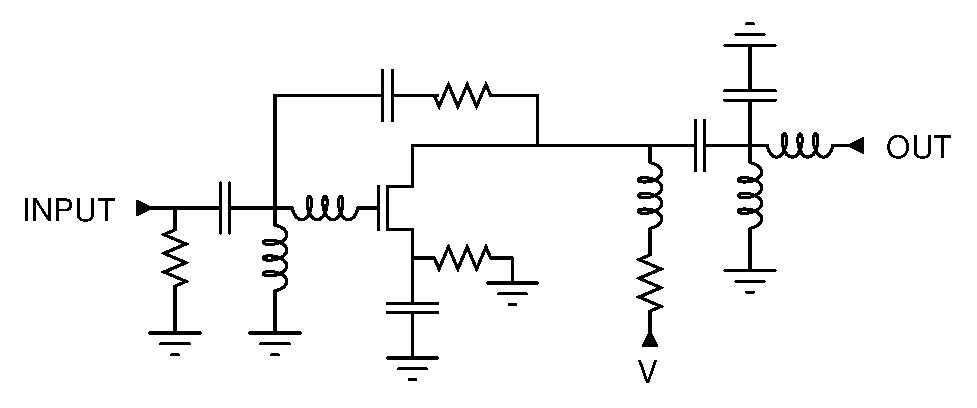
\includegraphics[width=0.85\textwidth]{fig/amplifiers/lo/sch_lo}
				\caption[LO-amplifier schematic]{Schematic of the LO-amplifier.}\label{fig:sch_lo}
			\end{figure}


			\begin{figure}[hbt!]
				\centering
				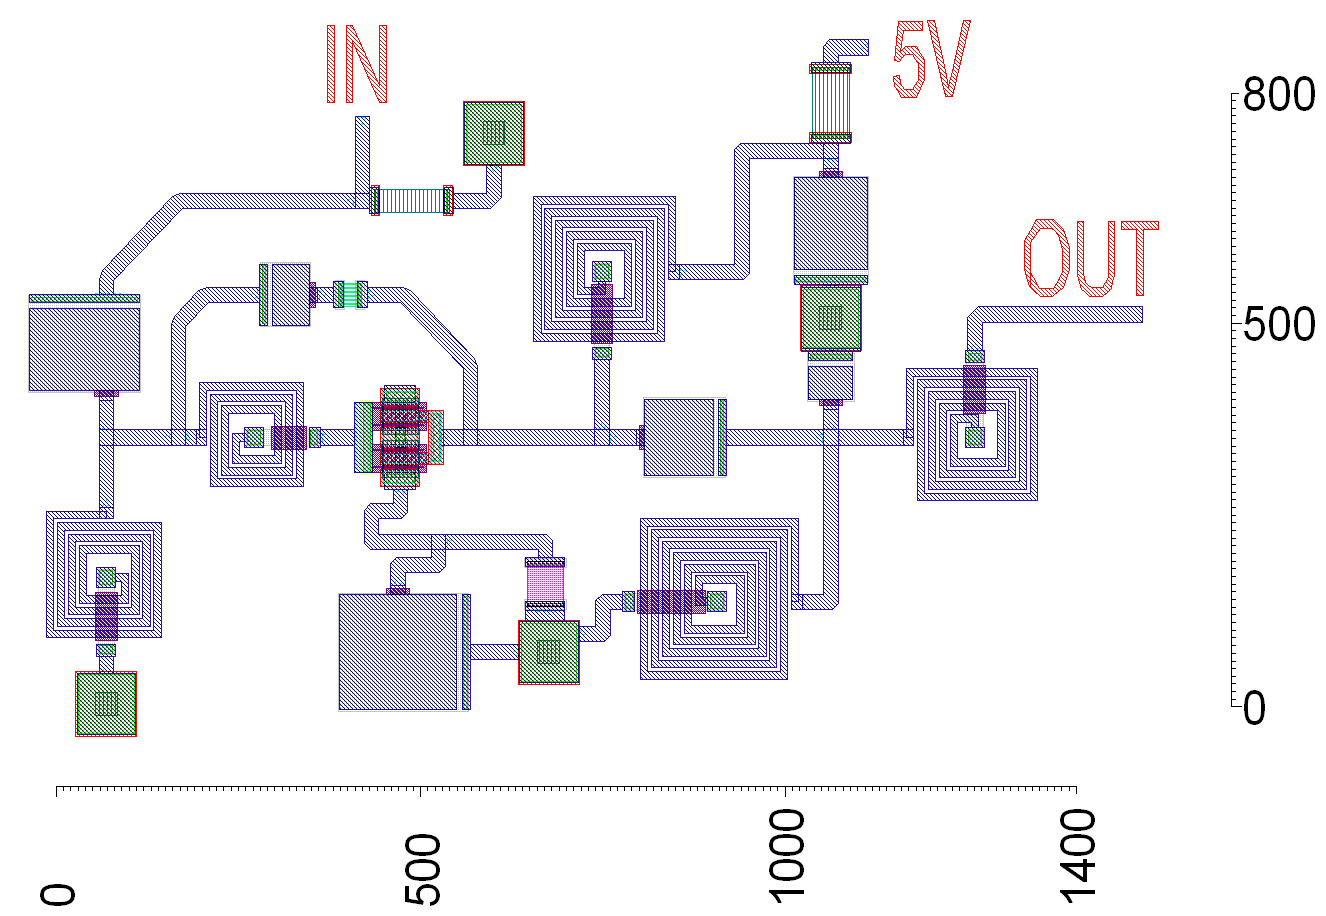
\includegraphics[width=1.0\textwidth]{fig/amplifiers/lo/layout}
				\caption[LO-amplifier layout]{The layout of the LO-amplifier with a weak parallel feedback, slightly elongated source for input matching, and a self-biasing scheme.\scalemum}\label{fig:lo_layout}
			\end{figure}



		\subsubsection{FET-configuration and matching networks}\label{sec:lo_fet_config}
			Large FETs are used for linear operation linear operation which is to be avoided for the compression technique to work.\autocite{maas98} In \autoref{fig:FET_size_S22}, the drain impedance for different FET-sizes is simulated. It shows that a smaller FET such as \unit[4$\times$25]{\mum} is a better conjugate match for the mixer since only reactive matching networks would be needed. However, such a small FET does not provide enough gain. Therefore a FET-size of \unit[4$\times$50]{\mum} is chosen.

	The input matching network consists of an L-shaped inductor-inductor network and a shunt-resistance. The length of the source is chosen such that input reflections are small. The output matching network needs to match the reactive gate of the mixing FET. This is done with a shunt capacitance and an inductance in series. The inductance to ground keeps the gate of the mixing FET at $v_{DC}=\unit[0]{V}$.
			\begin{figure}[hbt!]
				\centering
				%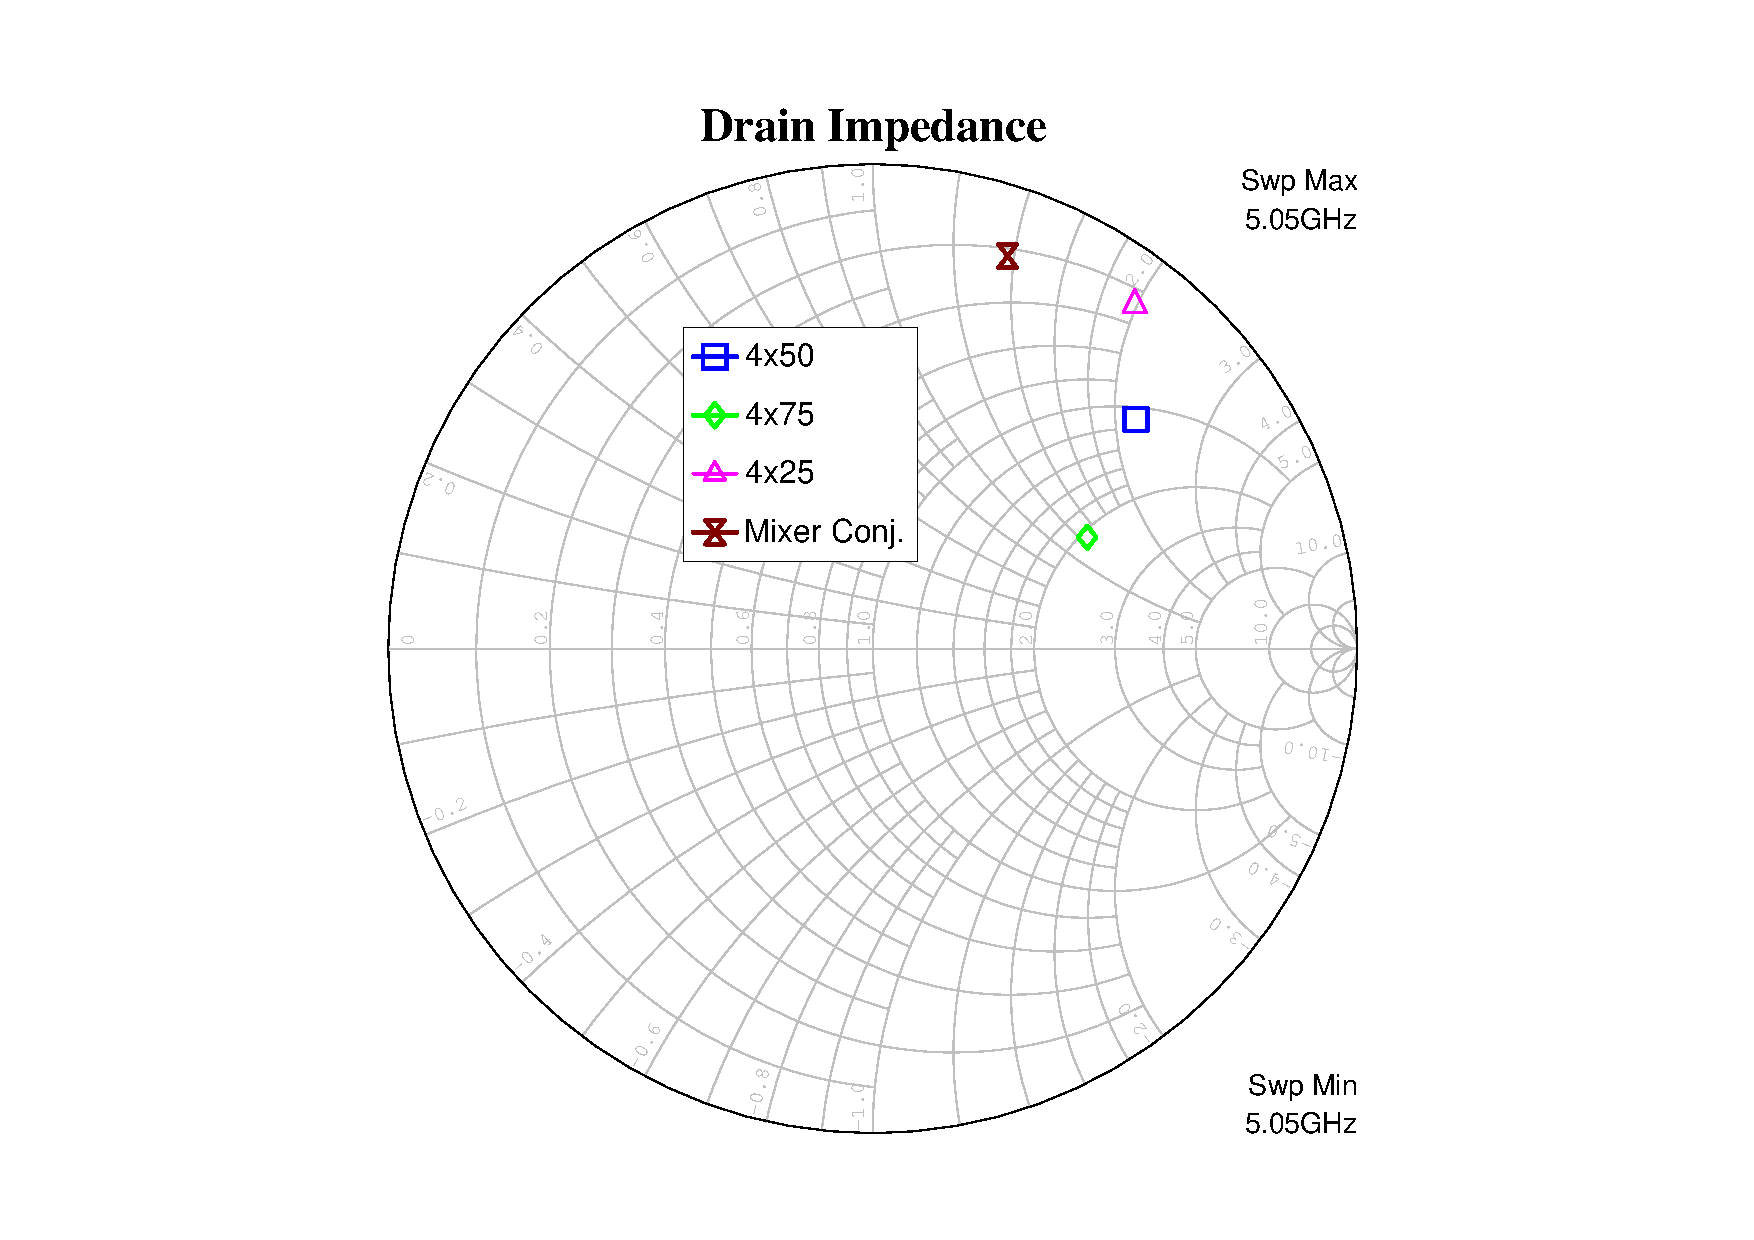
\includegraphics[trim=800 400 60 50, clip, width=0.5\textwidth]{fig/amplifiers/lo/FET_size_S22}
				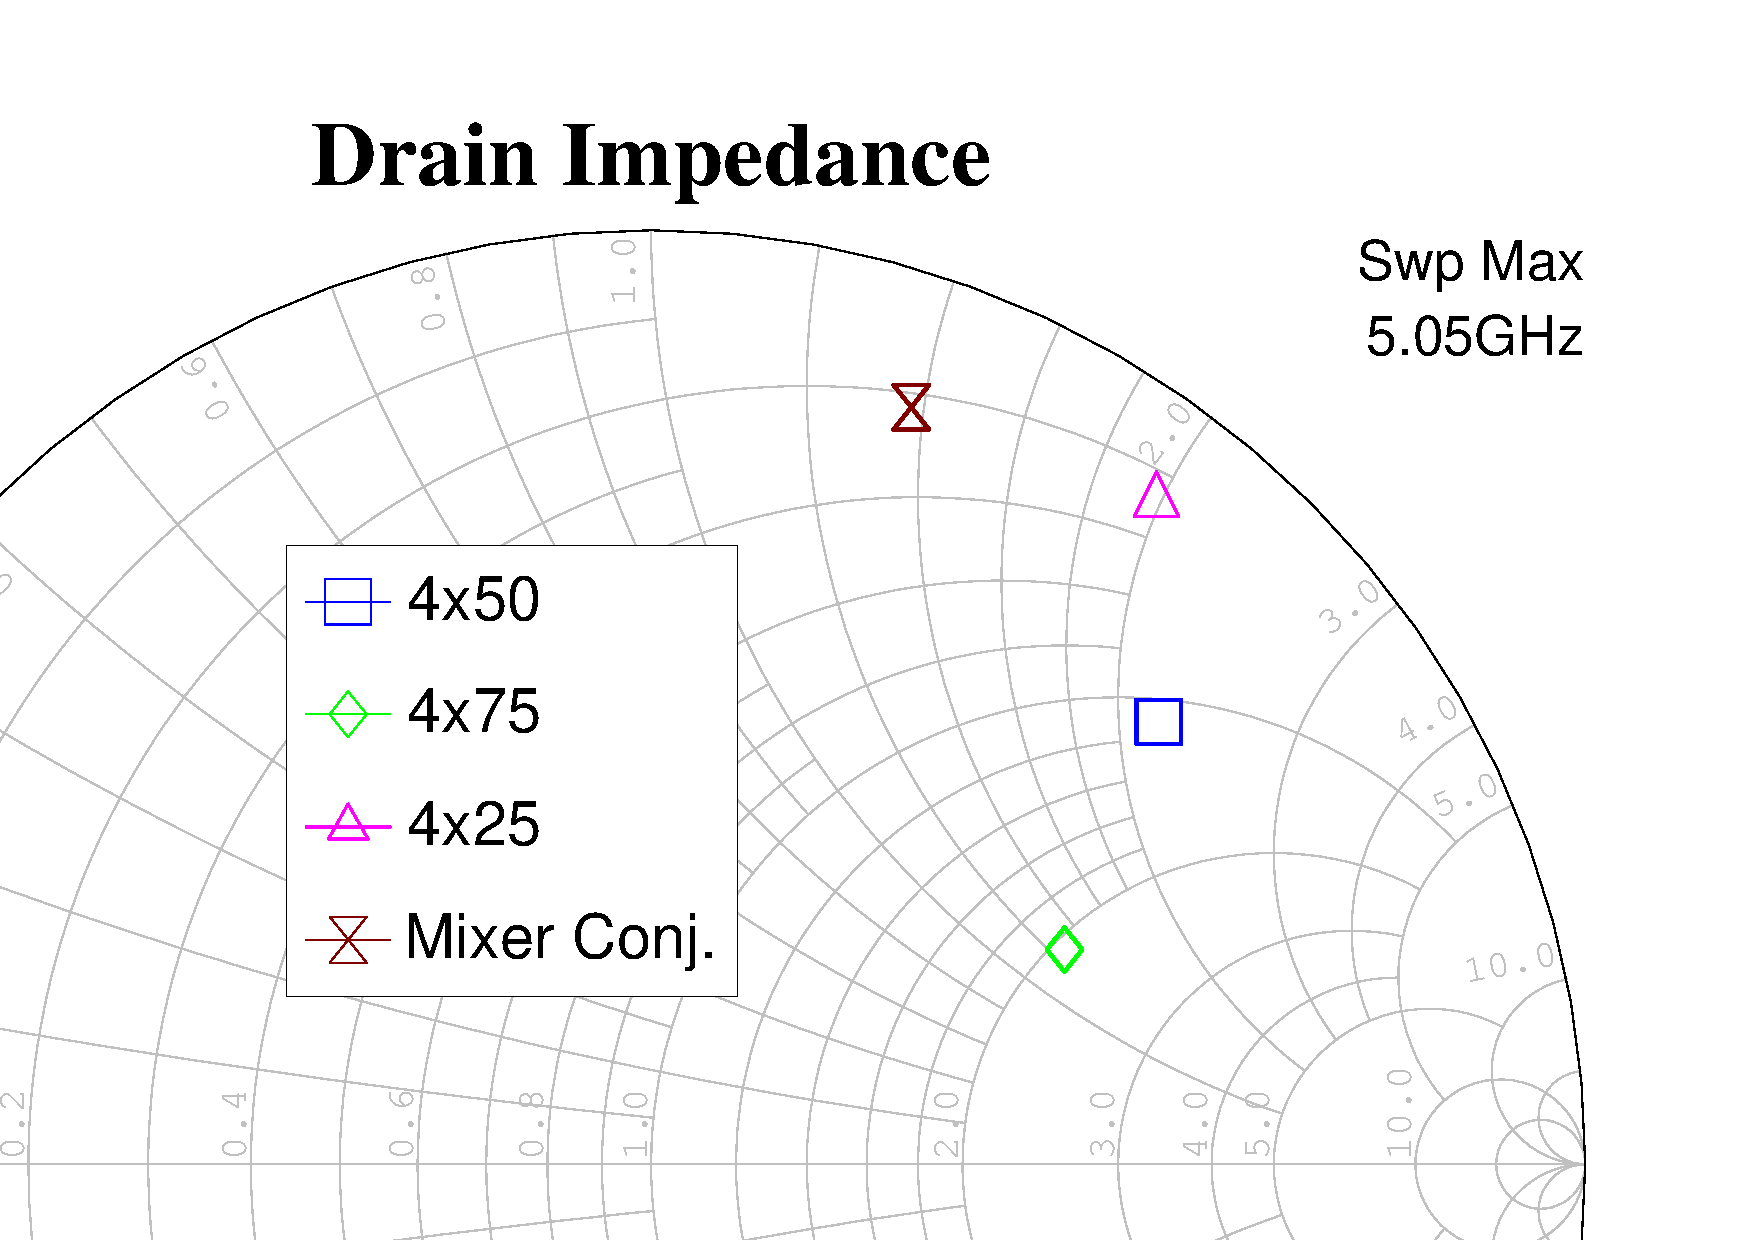
\includegraphics[width=1.0\textwidth]{fig/amplifiers/lo/FET_size_S22_zoom}
				\caption[Drain impedance for different FET's.]{The drain impedance for different FET-sizes. The \unit[4$\times$50]{\mum} and the \unit[4$\times$25]{\mum} FET-sizes make a good conjugate match for the mixer. However, \unit[4$\times$25]{\mum} does not provide enough gain.} \label{fig:FET_size_S22}
			\end{figure}

		\subsubsection{Bias point}
			The amplifier enters compression when applying a low $v_{ds}$ as seen in \autoref{fig:4x50_output_power} where output power is shown versus input LO power for different FET-bias points. The bias point $v_{gs}=\unit[-0.4]{V}$, $v_{ds}=\unit[2]{V}$ provides a signal in compression.

			\begin{figure}[hbt!]
				\centering
				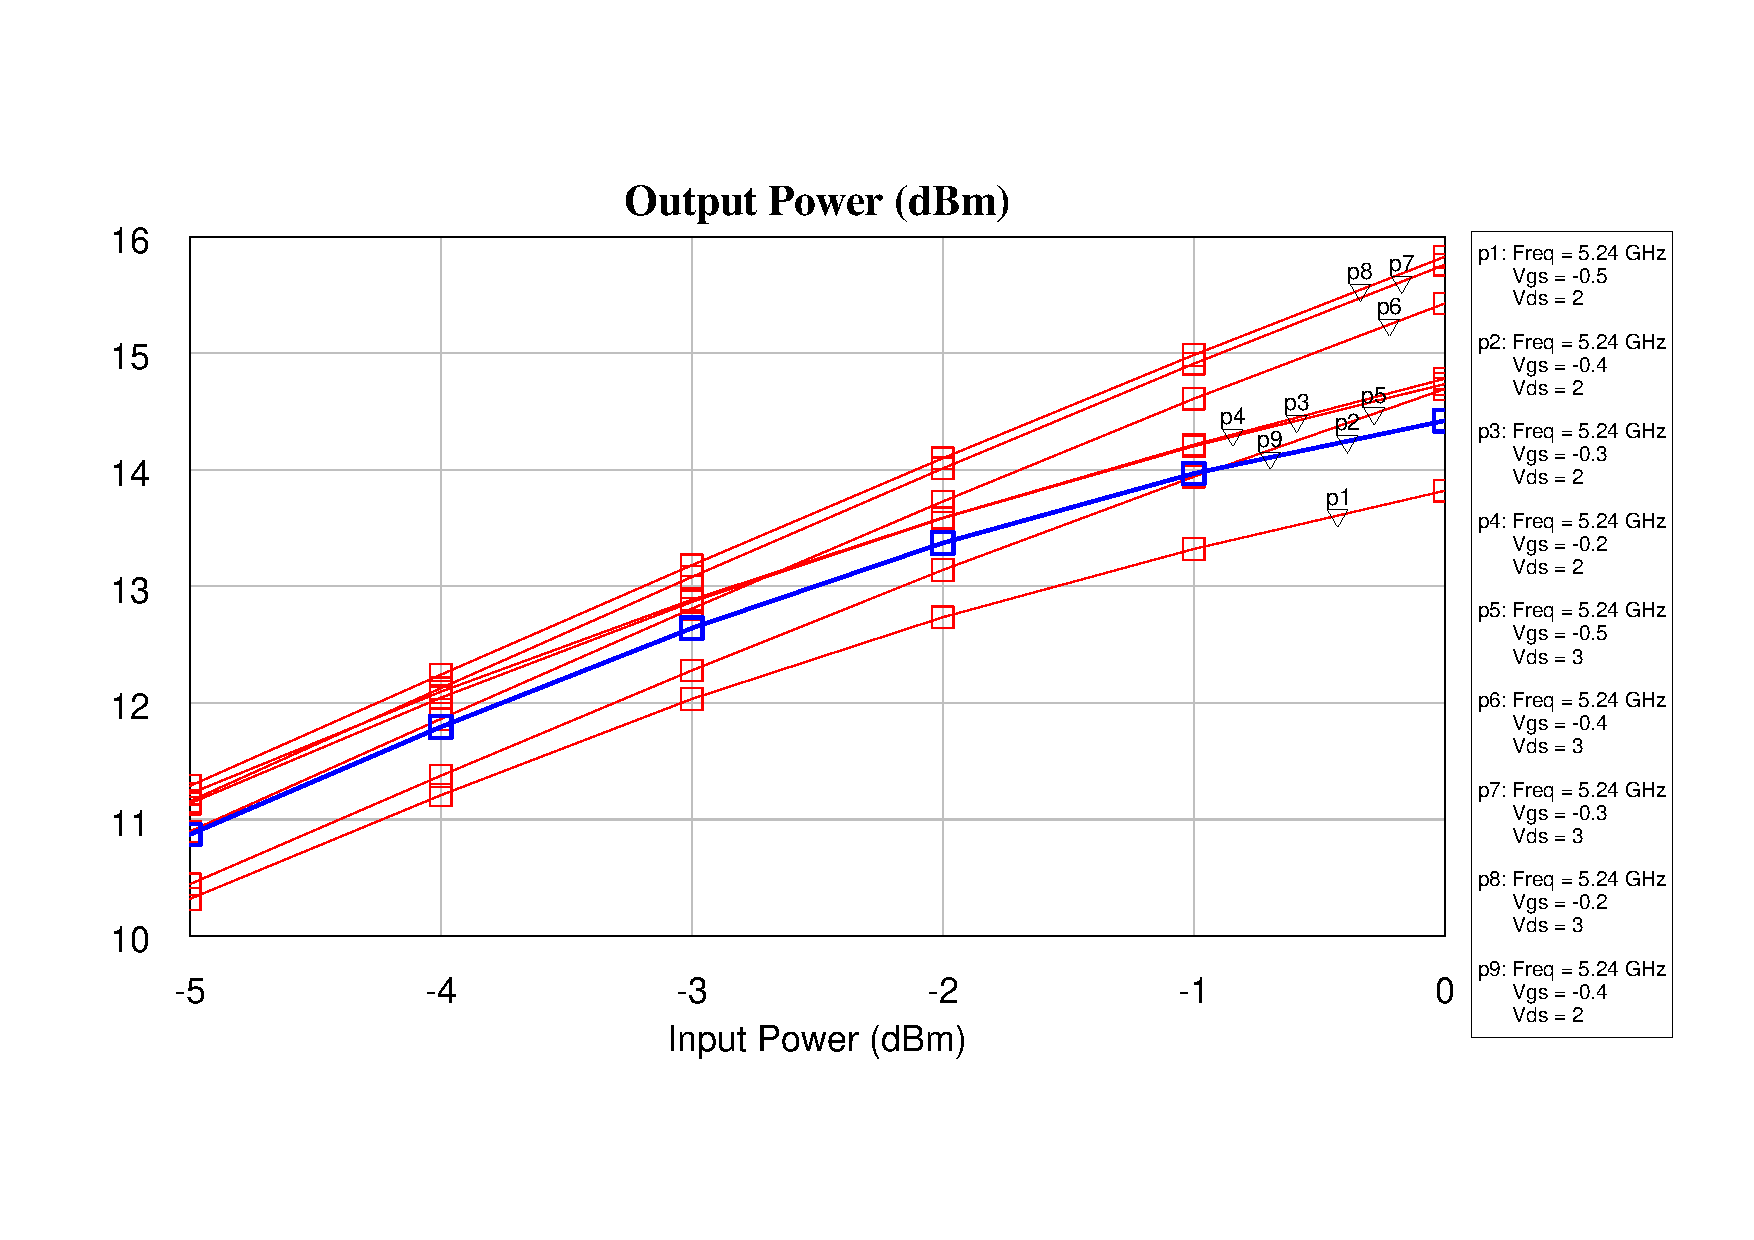
\includegraphics[trim=50 60 30 60, clip, width=0.9\textwidth]{fig/amplifiers/lo/4x50_output_power}
				\caption[Gain for different bias-points]{Output power for different bias points for the \unit[4$\times$50]{\mum} FET. The blue line represents the chosen bias-point $v_{gs}=\unit[-0.4]{V}$, $v_{ds}=\unit[2]{V}$.}\label{fig:4x50_output_power}
			\end{figure}



		\subsection{Simulation results}

			The simulation results for the LO-amplifier are presented in \autoref{tab:resultlo} for two ranges of input powers. The power delivered into the mixing FET is shown in \autoref{fig:lo_delivered_power} and it is clear that the amplifier is operating in compression for input powers of \unit[-2--0]{dBm} and less so for weaker input powers. The square-wave pulse is seen in figure \autoref{fig:lo_waveform}.

			The input reflections are shown in \autoref{fig:lo_reflections}. The reflections become a problem at higher frequencies and weaker input powers around \unit[-4]{dBm}. Good input matching is hard to achieve with the current amplifier design. As the load is changing depending on input power, it is difficult to match for all input powers. Emphasis has been placed on achieving a good match for $P_{LO}=\unit[-2]{dBm}$ which is considered to be the most likely input power.



%\autoref{tab:resultlo} presents LO-performance for input powers of $LO=\unit[-4$--$ -2]{dBm}$ and $LO=\unit[-2$--$0]{dBm}$. Delivered power and reflections are seen in \autoref{fig:lo_delivered_power} and \autoref{fig:lo_reflections}, respectively. The performance is good for higher input powers, for weaker input powers, the reflections become a problem at higher frequencies. Good input matching is hard to achieve with the current amplifier design. As the amplifier is running in compression, the load is changing depending on input power which makes it hard to match for all input powers. Emphasis has been placed on achieving a good match for $P_{lo}=\unit[-2]{dBm}$ which is considered to be the most likely input power. 	The square-wave pulse is seen in figure \autoref{fig:lo_waveform}.

			\begin{table}[hbt!]
				\caption[Simulation results of the LO-amplifier.]{Simulation results of the LO-amplifier.\disclaimer}
				\label{tab:resultlo}
				\centering
				\begin{tabular}{ l c c c c c c l } \toprule
					Parameter & Min. & Typ. & Max. & Min. & Typ. & Max. & Unit \\\midrule
					Frequency range & \multicolumn{3}{c}{5.04--5.54} & \multicolumn{3}{c}{5.24--5.44} & GHz \\
					Delivered Power & & & & & & \\
						\qquad @LO=\unit[-2--0]{dBm} 		& 4.0 & 4.8 & 5.5 & 4.6 & 5.0 & 5.4 & dB \\
						\qquad@LO=\unit[-4-- -2]{dBm} 		& 2.4 & 3.7 & 5.0 & 3.3 & 4.0 & 5.0 & dB \\
					Return loss input  & & & & & & \\
						\qquad @LO=\unit[-2--0]{dBm} 	& 13.5 & 17 & & 17 & 18 & & dB \\
						\qquad @LO=\unit[-4-- -2]{dBm} 	& 10.5 & 15 & & 13 & 16 & & dB \\
					Stability $K$@\unit[0--80]{GHz} & >1 & >1 &  & >1 & >1 &  & \\
					Power consumption &  & 100 &  & & 100 & & mW  \\\bottomrule
				\end{tabular}
			\end{table}

			\begin{figure}[hbt!]
				\centering
				\includerect{0.7\textwidth}{fig/amplifiers/lo/lo_delivered_power}
				\caption[Output power from LO-amplifier]{The power delivered into the mixer from the LO-amplifier for different frequencies and LO-input powers. It is measured in-between amplifier and mixer. The active frequencies are 5.04 to 5.54 GHz.}\label{fig:lo_delivered_power}
			\end{figure}
			\begin{figure}[hbt!]
				\centering
				\includerect{0.7\textwidth}{fig/amplifiers/lo/lo_waveform}
				\caption[Amplifier LO waveform]{Amplifier LO running in compression, producing a square-shaped output voltage waveform.}\label{fig:lo_waveform}
			\end{figure}

			\begin{figure}[hbt!]
				\centering
				\includerect{0.7\textwidth}{fig/amplifiers/lo/lo_reflections}
				\caption[Input reflections of LO-amplifier]{Input reflections of LO-amplifier, weaker input-powers and higher frequencies give larger reflections. The active frequencies are 5.04 to 5.54 GHz.}\label{fig:lo_reflections}
			\end{figure}



			\begin{figure}[hpt!]
				\centering
				\subfloat[][Mixer gain when spreading LO and mixer-FET at LO=-2 dBm.]{
					\includerect{0.5\textwidth}{fig/amplifiers/lo/lo_mixer_gain_spread_-2dBm}
					\label{fig:lo_mixer_gain_spread}
				}
				\subfloat[][Mixer compression when spreading LO- and mixer-FET for LO=-2 dBm.]{
					\includerect{0.5\textwidth}{fig/amplifiers/lo/lo_mixer_compression_spread_-2dBm_both_fets}
					\label{fig:lo_mixer_p1db_spread-2dBm}
				} \\
				\subfloat[][Mixer compression when spreading LO- and mixer-FET for LO=-4 dBm.]{
					\includerect{0.7\textwidth}{fig/amplifiers/lo/lo_mixer_compression_spread_-4dBm_both_fets}
					\label{fig:lo_mixer_p1db_spread-4dBm}
				}
				\caption{Conversion gain and compression point for the mixer when applying spread to the mixer- and LO-amplifier-FET. Using EM-models at $f_{rf}=\unit[3.2]{GHz}$. The observed spread in delivered LO-power is not present in \subref{fig:lo_mixer_p1db_spread-2dBm} ($P_{lo}=\unit[-2]{dBm}$) suggesting some threshold power is reached. For $P_{lo}=\unit[-4]{dBm}$, \subref{fig:lo_mixer_p1db_spread-4dBm}, the mixer's compression point is being affected by spread in the FETs.}\label{fig:lo_mixer_spread}
			\end{figure}





			The spread analysis, \autoref{fig:lo_spread}, suggests that the LO-amplifier is sensitive to variations. The delivered power may drop as much as \unit[2]{dB} for input powers of $\unit[-2]{dBm}$. %The frequency dependence of the spread is due to spread in the FET.
			However, when spreading the LO- and mixer-FET, the mixer conversion gain and compression are hardly affected (\autoref{fig:lo_mixer_spread}). This suggests that the power supplied to the mixer is above a threshold-power where it is fair to assume that stronger LO is less important\autocite{yhland1999}. However, for $P_{LO}=\unit[-4]{dBm}$, the mixer $P_{1dB}$ is affected and drops on one occasion to \unit[9.7]{dBm}.



	\subsection{Gain versus compression}
		It is possible to increase the amplifier's gain by increasing $v_{ds}$ a little, but this would not compress the signal as much. As seen in \autoref{fig:lo_mixer_gain_comparison}, the mixer gain for the compressed LO-signal has the same frequency dependence for different LO-powers. If the gain is increased, i.e. not so strong compression, the LO-signal will vary for different input signal and this causes the mixer-gain to behave badly  (Figure\autoref{fig:lo_mixergain_not_compressed}). When the LO-drive to the mixer becomes too large, the mixer-gain suffers.


				\begin{figure}[hpt!]
					\centering
					\subfloat[][Delivered power for LO-amplifier in compression ($v_{ds}=2$ V).]{
						\includerect{0.5\textwidth}{fig/amplifiers/lo/lo_delivered_power_compressed}
						\label{fig:lo_power_compressed}
					}
					\subfloat[][The delivered power for LO-amplifier in less compression ($v_{ds}=3$ V).]{
						\includerect{0.5\textwidth}{fig/amplifiers/lo/lo_delivered_power_not_compressed}
						\label{fig:lo_power_not_compressed}
					} \\
					\subfloat[][Mixer-gain for LO-amplifier in compression.]{
						\includerect{0.5\textwidth}{fig/amplifiers/lo/lo_mixergain_compressed}
						\label{fig:lo_mixergain_compressed}
					}
					\subfloat[][Mixer-gain for LO-amplifier in less compression. For LO=0 dBm the mixer-gain is starting to offset and drops drastically at higher frequencies.]{
						\includerect{0.5\textwidth}{fig/amplifiers/lo/lo_mixergain_not_compressed}
						\label{fig:lo_mixergain_not_compressed}
					} \\
					\caption{Comparison between a compressed and not as compressed LO by varying $V_{ds}$.}\label{fig:lo_mixer_gain_comparison}
				\end{figure}




	\subsection{Discussion}
		The key feature of the LO-amplifier is the square-waved pulse which helps to achieve a more linear mixer. The gain of the amplifier is somewhat low, this is attributed to the compression technique and the matching to the very reactive mixer FET. But having a more powerful LO, and thereby a greater mixer $P_{1dB}$, would not yield a great increase in the complete chip's compression point as the IF-amplifiers are the limiting factor. Also, for a stronger LO-drive, it is more difficult to reach adequate LO-isolation, see \autoref{fig:sysspectrum}.

		The amplifier can deliver some more gain in exchange for compression by increasing $v_{ds}$ a notch, see \autoref{fig:lo_mixer_gain_comparison}. However, there are repercussions on the mixer gain if the LO becomes too large. Therefore it might be of future interest to vary the \unit[5]{V}-bias voltage to achieve the desired bias-point. It is also possible to increase the gate-source voltage, $v_{gs}$, for some gain and increased power consumption.

		The interaction between mixer conversion gain and LO-amplifier is difficult to foresee which is why the matching network was modified many times and some adjustments to the diplexer's band-pass filter were made before acceptable performance was achieved.

		The literature states that a single ended FET resistive mixer has $P_{1dB}$ approximately \unit[4]{dB} above the LO-drive\autocite{radmanesh2002state} and the result of this LO-mixer construction approximately follows that rule. A $P_{1dB}$ of \unit[12]{dBm} at $P_{LO}=\unit[-4]{dBm}$, at center frequency and a \unit[3]{dB} attenuation in the diplexer says that the required LO should be \unit[5]{dBm}. The LO-amplifier outputs \unit[3.5]{dBm} at these conditions, and it is thought that the square-waved LO-drive accounts for the extra linearity.

		The reflections are tuned for an input power of \unit[-2]{dBm} but as the load changes for different input powers, it is difficult to achieve low reflections on all frequencies and for all input powers. Especially input powers of \unit[-4]{dBm} and high frequencies result in input reflections being \unit[-10]{dB}.

		The yield analysis, Figure \autoref{fig:lo_delivered_power_spread_-2dBm}, shows a large spread in delivered power, especially at high frequencies.  The spread at $P_{LO}=\unit[-2]{dBm}$ hardly affects the mixer conversion gain and compression point, suggesting that the delivered power is enough for this mixer. As the amplifier is much less in compression for $P_{LO}=\unit[-4]{dBm}$, the spread starts to affect the mixer performance (\autoref{fig:lo_mixer_spread}).

		%It is generally true that the compression technique and reflections behave much better for LO-signals in the band \unit[-2--0]{dBm}.
		Future work could investigate if it is possible to choose another bias-point with more gain and still maintain good compression and matching to the mixer. The parallel feedback could possibly be removed for some additional gain.  One solution to the large spread in the FET may be to use another bias-scheme which could be adjusted after production on a per-chip basis.
		For other MMIC-designs where the mixer requires a much stronger LO-drive, a two-stage LO-amplifier might be justified. The first stage would then supply high gain while the second stage compresses the signal.

	\section{Low noise IF-amplifier}
		\subsection{Introduction}
			All components of the MMIC should be as linear as possible. However, the noise figure in the system also requires attention. Together with the conversion loss in the mixer, the first IF-amplifier contributes with  most noise. This amplifier is therefore designed as a low noise amplifier (LNA). Linearity is still of high importance, which is why the amplifier should also have high $P_{1dB}$ and high $IIP_3$. As the IF-signal is a narrow band, the amplifier's bandwidth is only \unit[20]{MHz}.

		\subsection{Design}
			\subsubsection{Principle}
				The principle design of an LNA is to find the input matching network that minimizes the noise of the amplifier and at the same time matches to $S_{11}$. The first part of this would be finding the best FET size. In order to match to both $S_{11}$ and optimum noise, a series feedback is implemented.\autocite{lehmann85} The final noise figure of the amplifier is primarily the combination of both the losses in the input matching network and the noise inherent to the FET. The amplifier is biased according to the self-biasing scheme detailed in \autoref{sec:bias}.

			\subsubsection{Noise}\label{sec:if1noise}
				There is no noise model for the PPH25 FET. The only data available are measurements of a \unit[4$\times$75]{\mum} FET provided by UMS. To estimate the amplifier's noise the PH25 model is used. This model together with the similarity in behaviour between the PH25 and the PPH25 FET gives a crude estimate of the noise figure. The position of the $\Gamma_{opt}$ is approximately the same for the different processes. The noise increases faster in the PPH25 case as mismatch increases (see \autoref{fig:if1noisematch}). Approximately \unit[0.5]{dB} is added to the noise simulated with the PH25 FET to get the PPH25 noise, provided the mismatch is not too large.

			\begin{figure}[hbt!]
				\centering
				%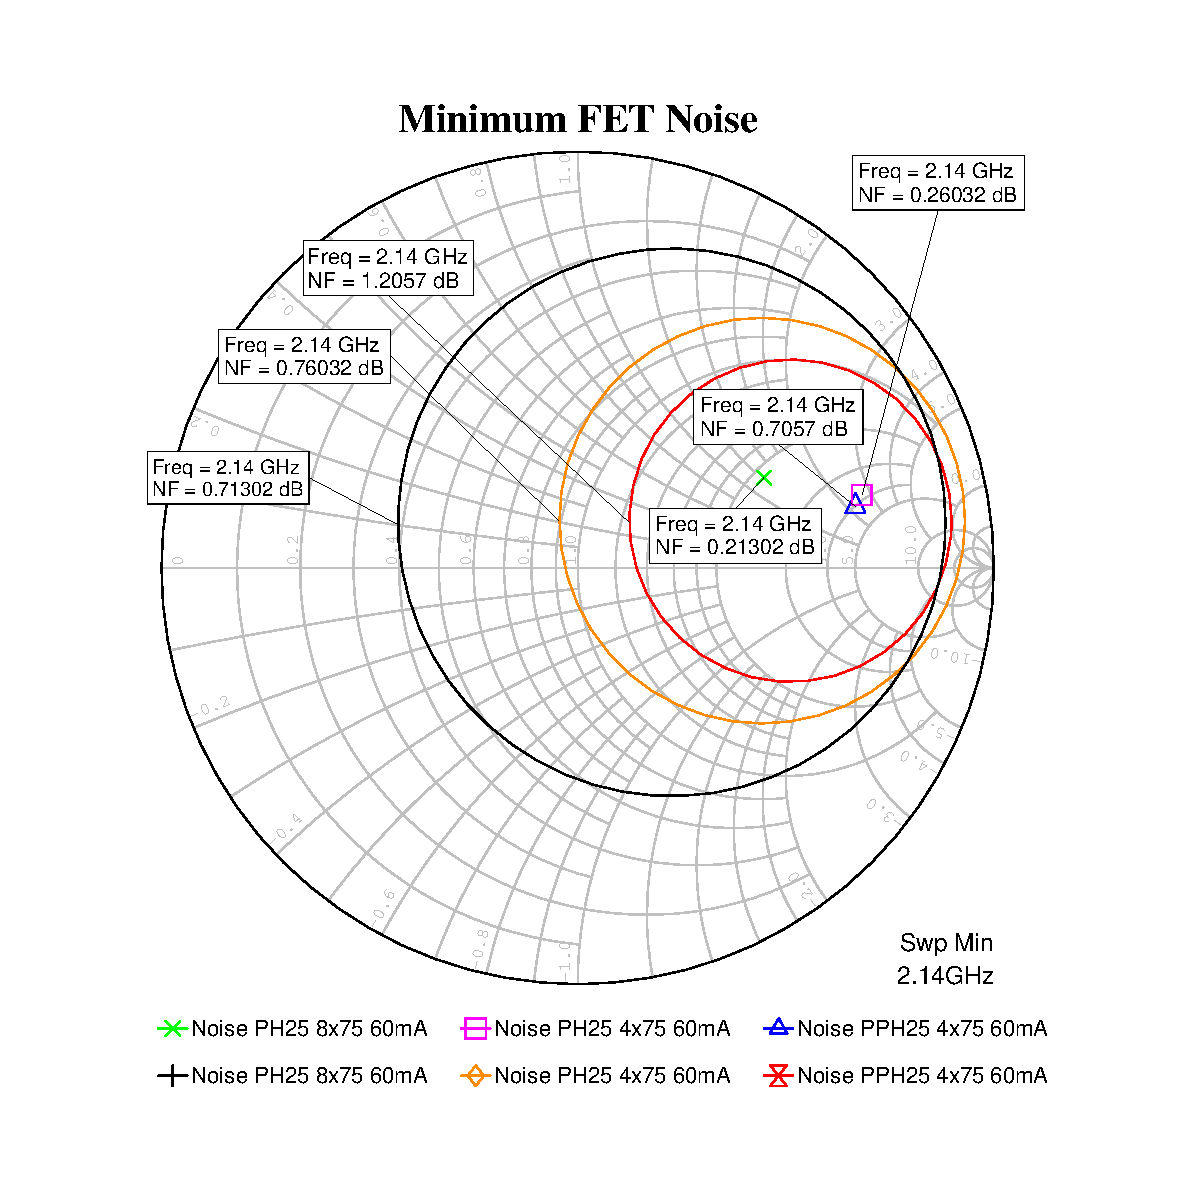
\includegraphics[width=1.0\textwidth]{fig/amplifiers/if1/noisematch}
				\includesmith{0.8\textwidth}{fig/amplifiers/if1/noisematch}
				\caption[$\Gamma_{opt}$ and constant noise circles for UMS FETs.]{$\Gamma_{opt}$ and constant noise circles for different UMS FET, both PH25 and PPH25. Both the absolute noise and the noise increase with mismatch are greater for PPH25. The \unit[8$\times$75]{\mum} is the biggest FET available. It has the lowest inherent noise, the most conveniently placed $\Gamma_{opt}$ and is the most linear device (see \autoref{sec:mixerdevice}).}\label{fig:if1noisematch}
			\end{figure}

			\subsubsection{FET selection and input network}
				Based on the noise properties of the FETs and previous work with the PH25 process\autocite{gustavsson07}, the \unit[8$\times$75]{\mum} FET is chosen for the amplifier. Fortunately, both low noise and linear operation favours a large device. The input network is a simple L-shaped inductor-inductor impedance matching network.

			\subsubsection{Attenuator}
				The chip design requires the amplifier to have a certain gain. If the gain of this amplifier is higher, the total $IIP_3$ will suffer and if it is lower the final noise will increase. As the amplifier's gain is higher than the specified \unit[12]{dB}, an attenuator consisting of two resistors is placed at the end. It is designed to optimize the input and output matching as well as add to the stability.\autocite{delpy06} An alternative to an attenuator is parallel feedback. This design would however degrade the noise figure and has therefore been discarded.

		\subsection{Schematics and layout}
			The schematic of amplifier IF1 is shown in \autoref{fig:if1schematic}. The corresponding layout is found in \autoref{fig:if1layout}.

			\begin{figure}[hbt!]
				\centering
				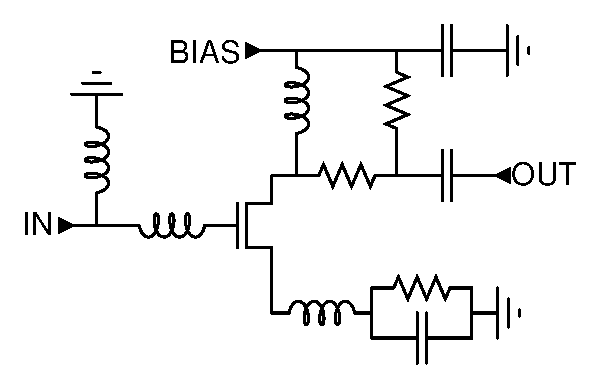
\includegraphics[width=0.7\textwidth]{fig/amplifiers/if1/sch_if1}
				\caption[Amplifier IF1 schematic.]{Schematic of amplifier IF1.}\label{fig:if1schematic}
			\end{figure}

			\begin{figure}[hbt!]
				\centering
				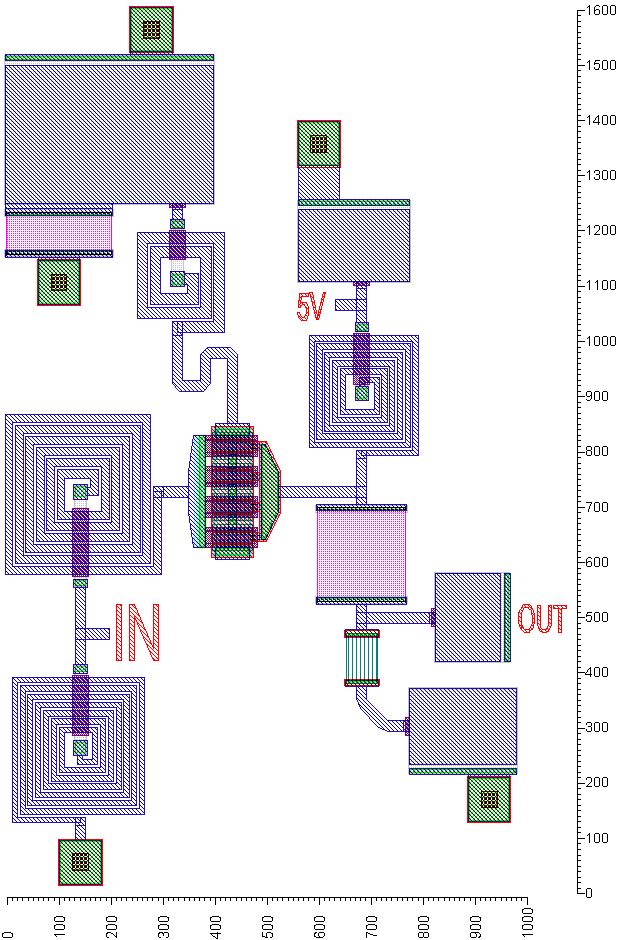
\includegraphics[width=0.7\textwidth]{fig/amplifiers/if1/layout}
				\caption[Amplifier IF1 layout.]{Layout of amplifier IF1.\scalemum}\label{fig:if1layout}
			\end{figure}

		\subsection{Simulation results}
			The simulated performance of amplifier IF1 is found in \autoref{tab:resultif1}. Spread analysis is reported in \autoref{sec:yieldif1} together with plots of the simulation data.  The full spectrum gain is plotted in \autoref{fig:if1gain}.

			\begin{table}[hbt!]
				\caption[Simulation results for amplifier IF1.]{Simulation results for amplifier IF1.\disclaimer}
				\label{tab:resultif1}
				\centering
				\begin{tabular}{ l c c c l } \toprule
					Parameter & Min. & Typ. & Max. & Unit \\\midrule
					Frequency range & \multicolumn{3}{c}{2.04--2.24} & GHz \\
					Gain & 11.2 & 11.5 & 11.8 & dB \\
					Return loss input & 12.1 & 14.4 &  & dB \\
					Return loss output & 16.5 & 16.9 &  & dB \\
					Stability $K$@\unit[0--80]{GHz} & >1 & >1 &  &  \\
					$P_{1dB}$ (input) & 5.7 & 6.5 &  & dBm \\
					$IIP_3$ & 19.0 & 19.5 &  & dBm \\
					Power consumption &  & 290 & 290 & mW \\
					Noise figure (estimate) &  & 1.5 & 1.8 & dB \\\bottomrule
				\end{tabular}
			\end{table}

			\begin{figure}[hbt!]
				\centering
				\includerect{0.7\textwidth}{fig/amplifiers/if1/widegain}
				\caption[Amplifier IF1 gain.]{Gain of amplifier IF1.}\label{fig:if1gain}
			\end{figure}

%		\subsubsection{Source Pull Analysis}
%			A source pull analysis that plots constant noise figure curves along with the optimal $S_{11}$ input match has been conducted (\autoref{fig:if1sourcepull}). The contours show that low noise and good matching overlap fairly good. This is overlap is mostly due to the series feedback.

		\subsection{Discussion}
			The narrowband property of the amplifier enables a design in which parallel feedback can be omitted. This has a good impact on the noise figure but it also gives a steep gain slope and a gate that is hard to match. One consequence is that the matching inductors become very large which in turn increases the noise figure as the UMS inductors have a somewhat low quality factor Q. Another consequence is that if the frequency characteristics shift only \unit[100]{MHz} during fabrication, the performance of the amplifier will change dramatically. Detailed frequency dependence can be found in \autoref{sec:yieldif1}.

			A noise figure of \unit[1.5]{dB} can by LNA-standards not be considered low. In the PH25 process, this value could very well be cut in half.\autocite{kyuko96} Still, amplifier IF1 is not only designed for low noise, but also to be linear. This leads to a compromise in which the slightly noisier power-PH25 process without noise models is used.

%			\begin{figure}[hbt!]
%				\centering
%				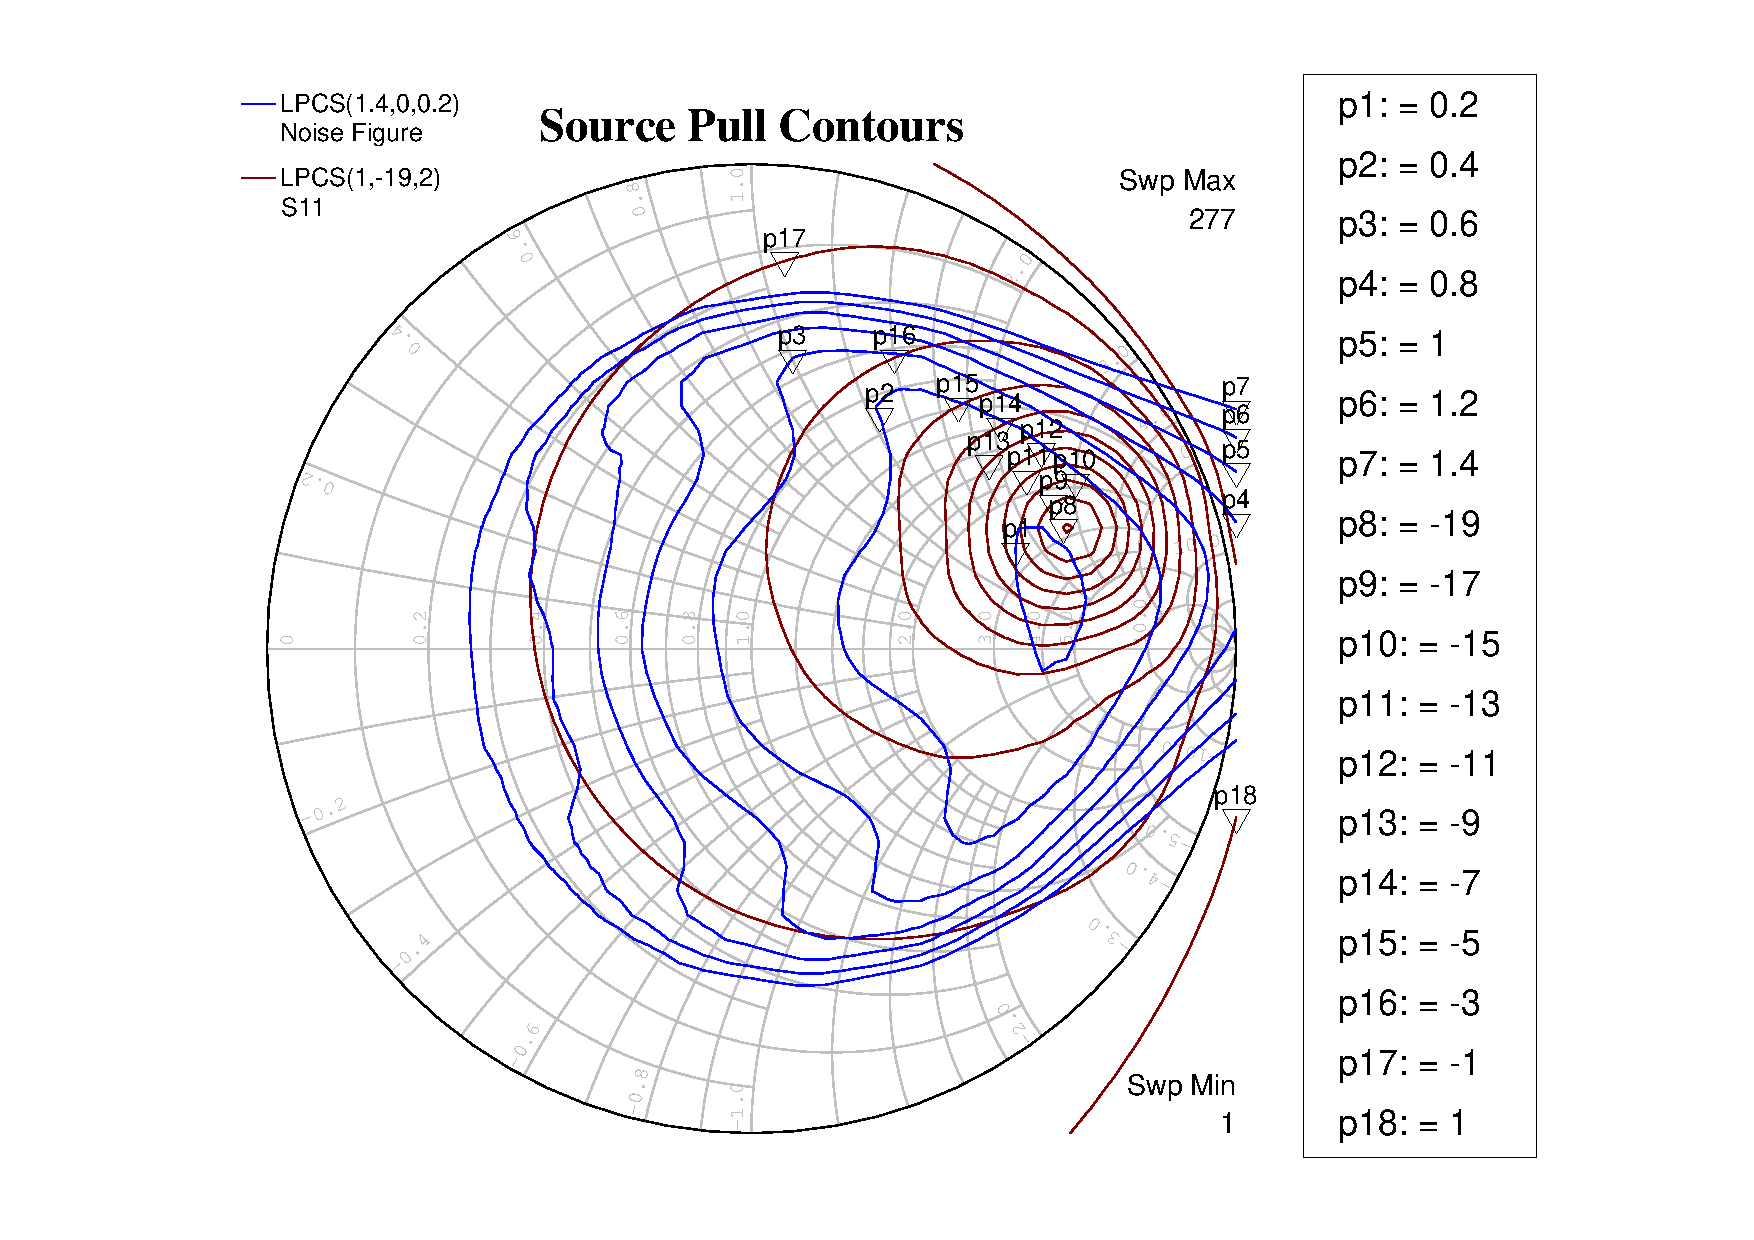
\includegraphics[width=1.0\textwidth]{fig/amplifiers/if1/sourcepull}
%				\caption[Source pull diagram for optimal noise figure.]{Source pull diagram for optimal noise figure and input match. The the optimal points for the two quantities overlap fairly good. The noise value is not that sensitive to the source impedance. The area for which the value stays below \unit[0.4]{dB} is large. It is therefore likely that the noise originating from the components matching the input of the amplifier will cause more noise than mismatching the input itself will.}\label{fig:if1sourcepull}
%			\end{figure}

	\section{High-power IF-amplifier}
		\subsection{Introduction}\label{sec:if2power}
			The last amplification stage has, together with the mixing component, the biggest impact on the overall chip linearity. As discussed earlier, the more DC-power provided, the more linear the operation becomes. Because the signal has already been amplified once, the overall noise figure is not very sensitive to the noise here. High power devices generate a lot of heat and this has to be taken into consideration.

		\subsection{Design}
			\subsubsection{Principle}
				To design a high linearity amplifier a method similar but opposite to the one used to design an LNA is used. Instead of matching the input to the noise optimum, the output is matched to peak $P_{1dB}$. The first step is to create a stable and input-matched circuit. Feedback circuits are used to control the gain and the linearity of the amplifier. Using this amplifier load-pull simulations are made for different bias points. This way it is possible to see which bias point and output matching network give the most linear operation.\autocite{anand08}

			\subsubsection{Thermal considerations}
				Calculations performed on the FETs' junction temperatures show that in order to handle the available DC-power and the specified ambient temperature, there has to be two FETs. With only one \unit[8$\times$75]{\mum} FET, the junction temperature $T_j$ exceeds \unit[170]{$^\circ C$}, which is the maximum rating for a GaAs FET. $T_j$ is calculated using thermal resistance models\autocite{fukui80}, where $T_0$ is set to $\unit[100]{^\circ C}$:

				\begin{equation}
					T_j=T_0+P_{FET}R_{TH}
				\end{equation}

				$P_{FET}$ is the power dissipated over the FET and $R_{TH}$ is the FETs thermal resistance according to the models. $T_0$, the temperature on the backside of the chip, is the sum of the ambient temperature and the estimated thermal resistance in the circuit board and the chip package. If the total thermal resistance is $\unit[15]{^\circ C}$, the chip can handle an ambient temperature of $\unit[100]{^\circ C}-\unit[15]{^\circ C}=\unit[85]{^\circ C}$.

				With two \unit[6$\times$75]{\mum} FETs, the maximum $T_j$ becomes $\approx$ \unit[150]{$^\circ C$}, which is a high although manageable temperature. Two FETs placed in parallel can be viewed as one big FET with the number of gate fingers equal to the sum of the parts, thus resulting in an equivalent \unit[12$\times$75]{\mum} FET.

			\subsubsection{Feedback and bias}
				The second IF-amplifier is biased in the same manner as the first one, described in \autoref{sec:bias}. This amplifier has both series feedback and parallel negative feedback. Though very small, the inductor on the source creating the series feedback is needed for stability and gain control. The parallel feedback that connects the drain to the gate has an attenuating resistance and a capacitance for DC blocking. The purpose of this feedback is to simplify matching and to provide high bandwidth. Although the signal is of a narrowband frequency, it is preferable if not both amplifiers' gain are frequency sensitive. The parallel feedback also makes the amplifier less stable.

				The FETs decrease in gain slightly as the temperature rises. To compensate for this loss, a resistor of GaAs type is chosen for the parallel feedback. This resistor has a positive temperature gradient. This way the decrease in gain is reduced by the smaller feedback.

		\subsection{Schematic and layout}
			The schematic of amplifier IF2 is shown in \autoref{fig:if2schematic}. The corresponding layout is found in \autoref{fig:if2layout}.

			\begin{figure}[hbt!]
				\centering
				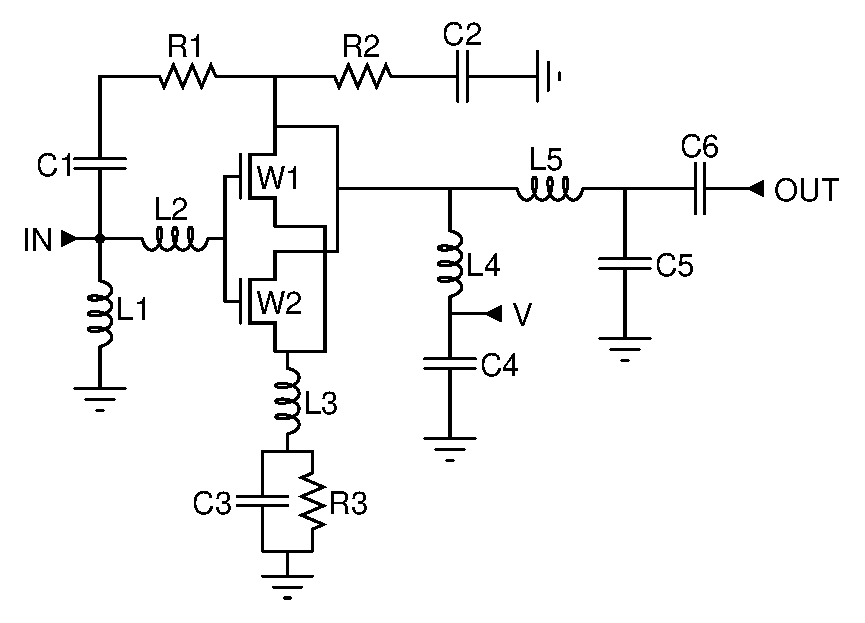
\includegraphics[width=0.75\textwidth]{fig/amplifiers/if2/sch_if2}
				\caption[Amplifier IF2 schematic.]{Schematic of amplifier IF2.}\label{fig:if2schematic}
			\end{figure}

			\begin{figure}[hbt!]
				\centering
				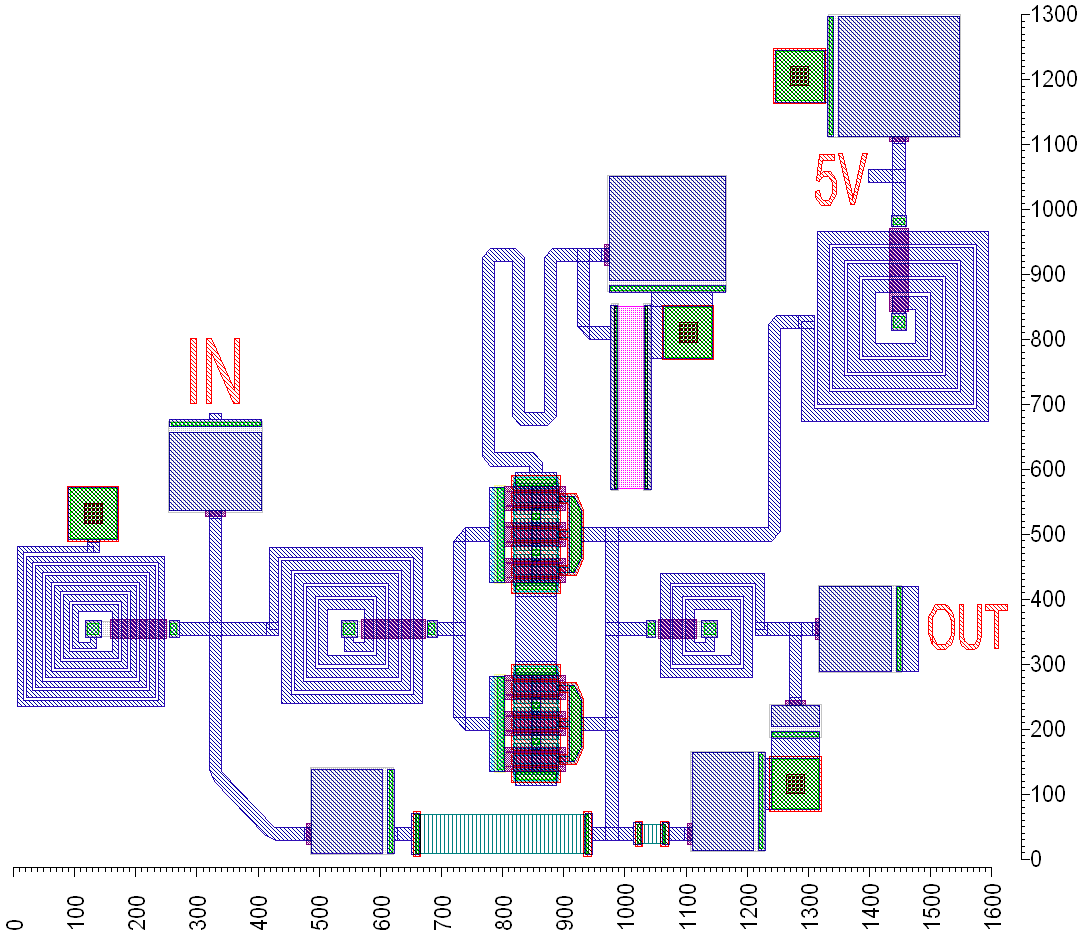
\includegraphics[width=1.0\textwidth]{fig/amplifiers/if2/layout}
				\caption[Amplifier IF2 layout.]{Layout of amplifier IF2.\scalemum}\label{fig:if2layout}
			\end{figure}

		\subsection{Simulation results}
			\subsubsection{Performance overview}
				The simulated performance of amplifier IF2 is seen in \autoref{tab:resultif2}. Spread analysis is reported in \autoref{sec:yieldif2} along with plots of the simulation data. The gain is plotted in \autoref{fig:if2gain}. The flat top of the gain is due to the parallel feedback.

				\begin{table}[hbt!]
					\caption[Simulation results of amplifier IF2.]{Simulation results of amplifier IF2.\disclaimer}
					\label{tab:resultif2}
					\centering
					\begin{tabular}{ l c c c l }\toprule
						Parameter & Min. & Typ. & Max. & Unit \\\midrule
						Frequency range & \multicolumn{3}{c}{2.04--2.24} & GHz \\
						Gain & 12.0 & 12.1 & 12.1 & dB \\
						Return loss input & 24.9 & 25.5 &  & dB \\
						Return loss output & 18.0 & 19.7 &  & dB \\
						Stability $K$@\unit[0--70]{GHz} & >1 & >1 &  &  \\
						$P_{1dB}$ (input) & 10.4 & 10.4 &  & dBm \\
						$IIP_3$ & 22.0 & 22.5 &  & dBm \\
						Power consumption &  & 550 & 550 & mW \\
						Noise figure (estimate) &  & 2.0 & 2.3 & dB \\\bottomrule
					\end{tabular}
				\end{table}

				\begin{figure}[hbt!]
					\centering
					\includerect{0.7\textwidth}{fig/amplifiers/if2/widegain}
					\caption[Amplifier IF2 gain.]{Gain of amplifier IF2.}\label{fig:if2gain}
				\end{figure}

			\subsubsection{Linearity analysis}
				The \unit[1]{dB}-compression point, $P_{1dB}$, is simulated for different $i_{ds}$ (\autoref{fig:if2p1dbvspower}). A load pull analysis with both the output matching and $P_{1dB}$ analysed is shown in \autoref{fig:if2lp}. The analysis shows the importance of choosing a correct, and in this case high power, bias point to optimize the two quantities. From the three plots combined it can be seen that the linearity increases dramatically with increased power until peak $P_{1dB}$ is aligned with optimum output match. After that, the increase is only linear. This overall linearity increase agrees with the discussion about power utilisation in \autoref{sec:power}.

				\begin{figure}[h!]
					\centering
					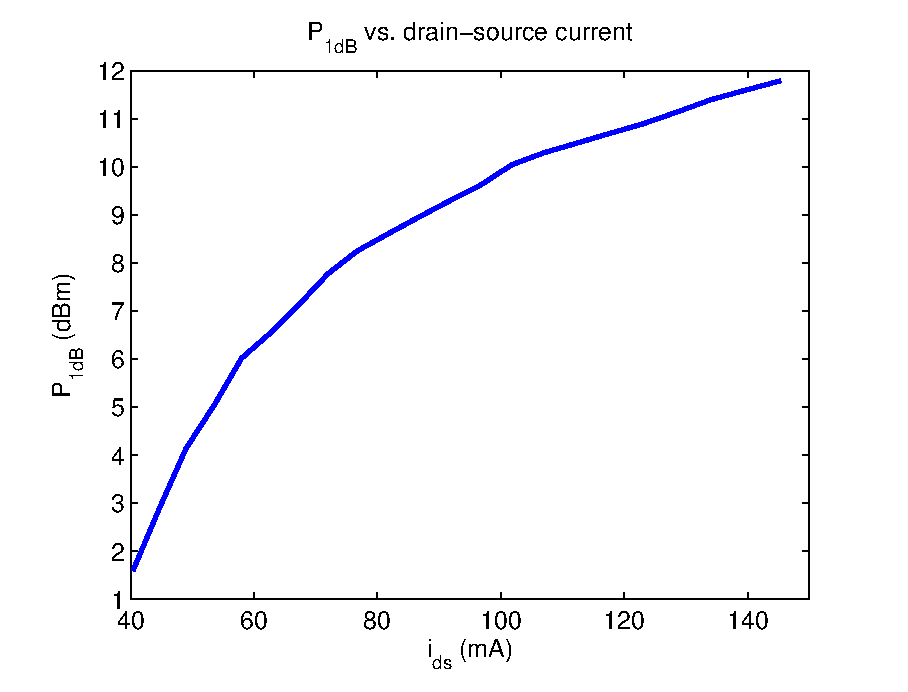
\includegraphics[width=0.7\textwidth]{fig/amplifiers/if2/p1dbvscurrent}
					\caption[Amplifier IF2 $P_{1dB}$ versus $i_{ds}$.]{Amplifier IF2 $P_{1dB}$ versus $i_{ds}$. The increase with increased power is non-linear in the beginning. From approximately \unit[90]{mA} the increase is linear.}\label{fig:if2p1dbvspower}
				\end{figure}

				\begin{figure}[h!]
					\centering
					\subfloat[][Power consumption 400 mW corresponding to drain-source current 80 mA.]{
						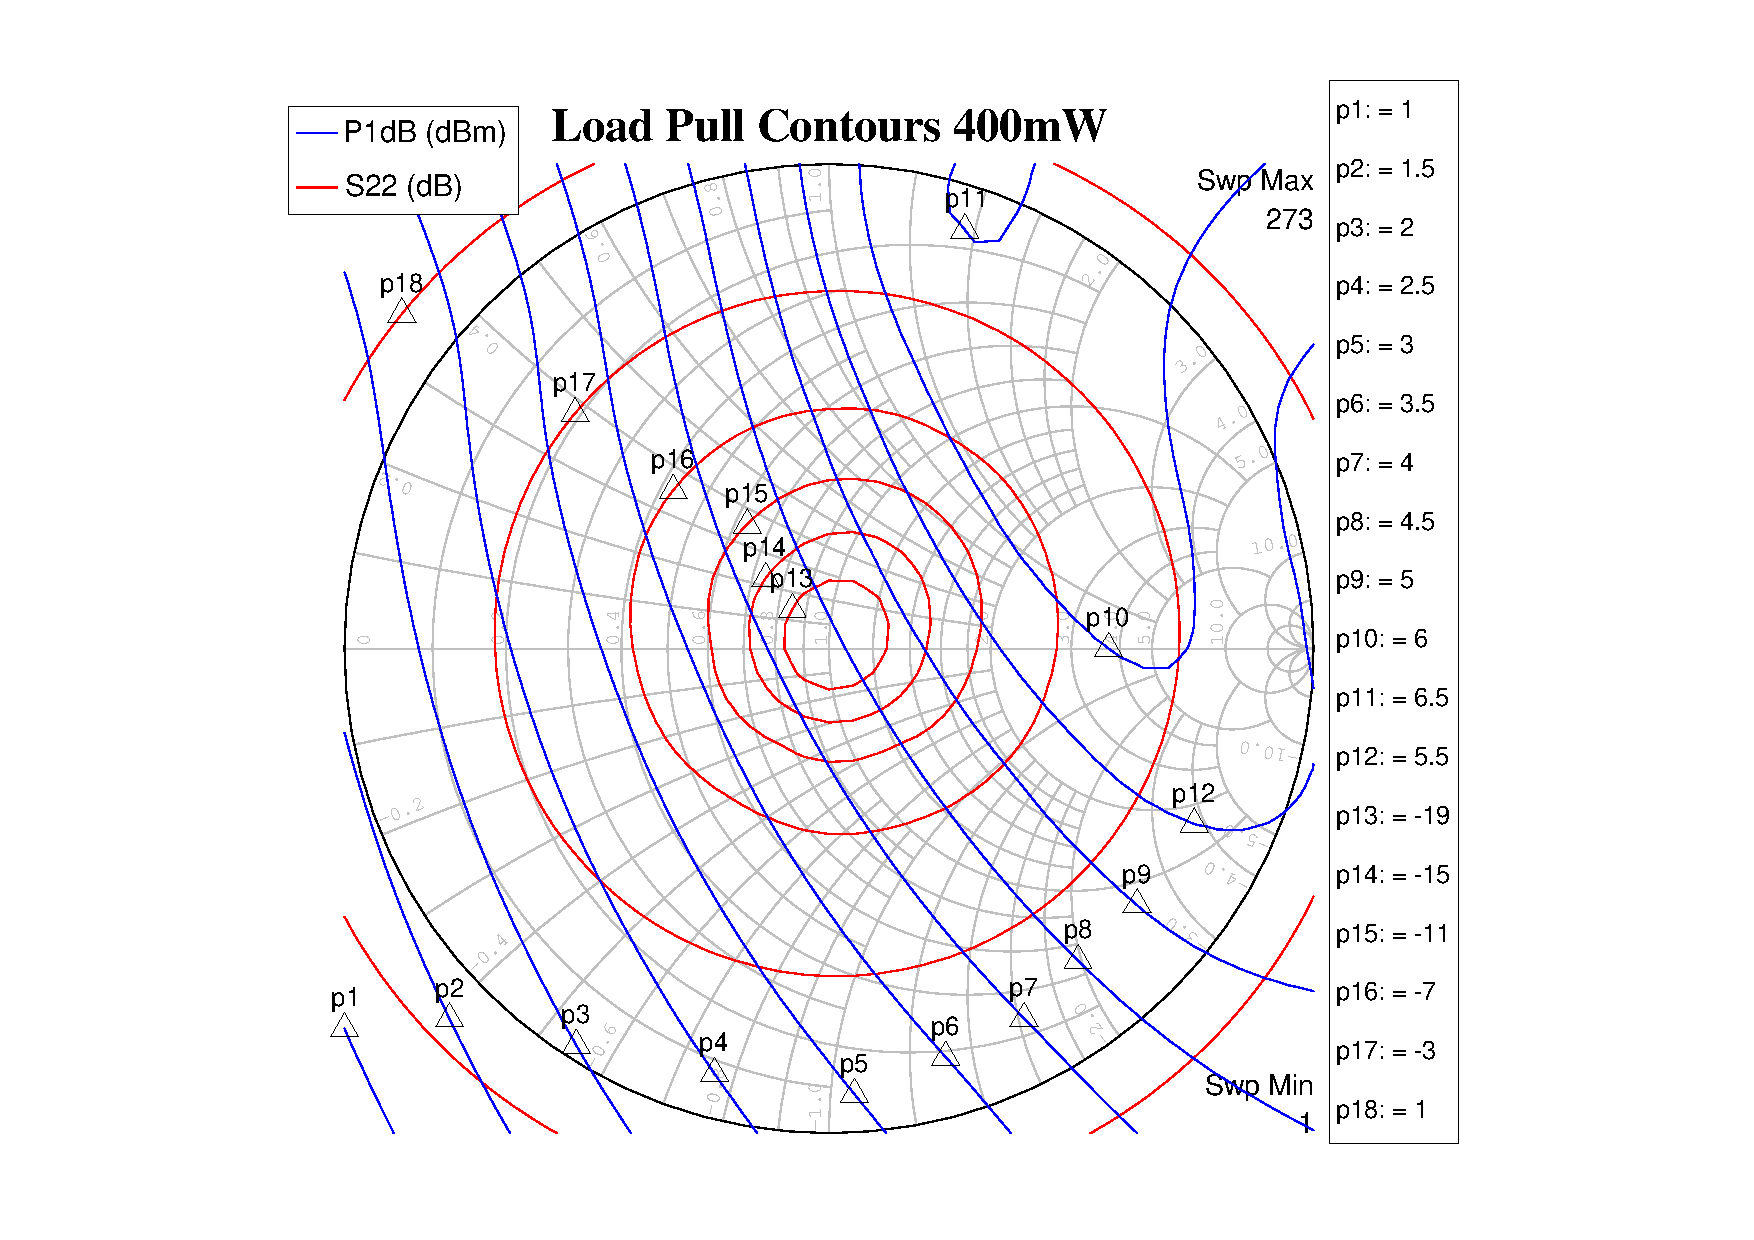
\includegraphics[trim=120 35 125 35, clip, width=0.7\textwidth]{fig/amplifiers/if2/loadpull400}
						\label{fig:if2lp400}
					} \\
					\subfloat[][Power consumption 550 mW corresponding to drain-source current 110 mA.]{
						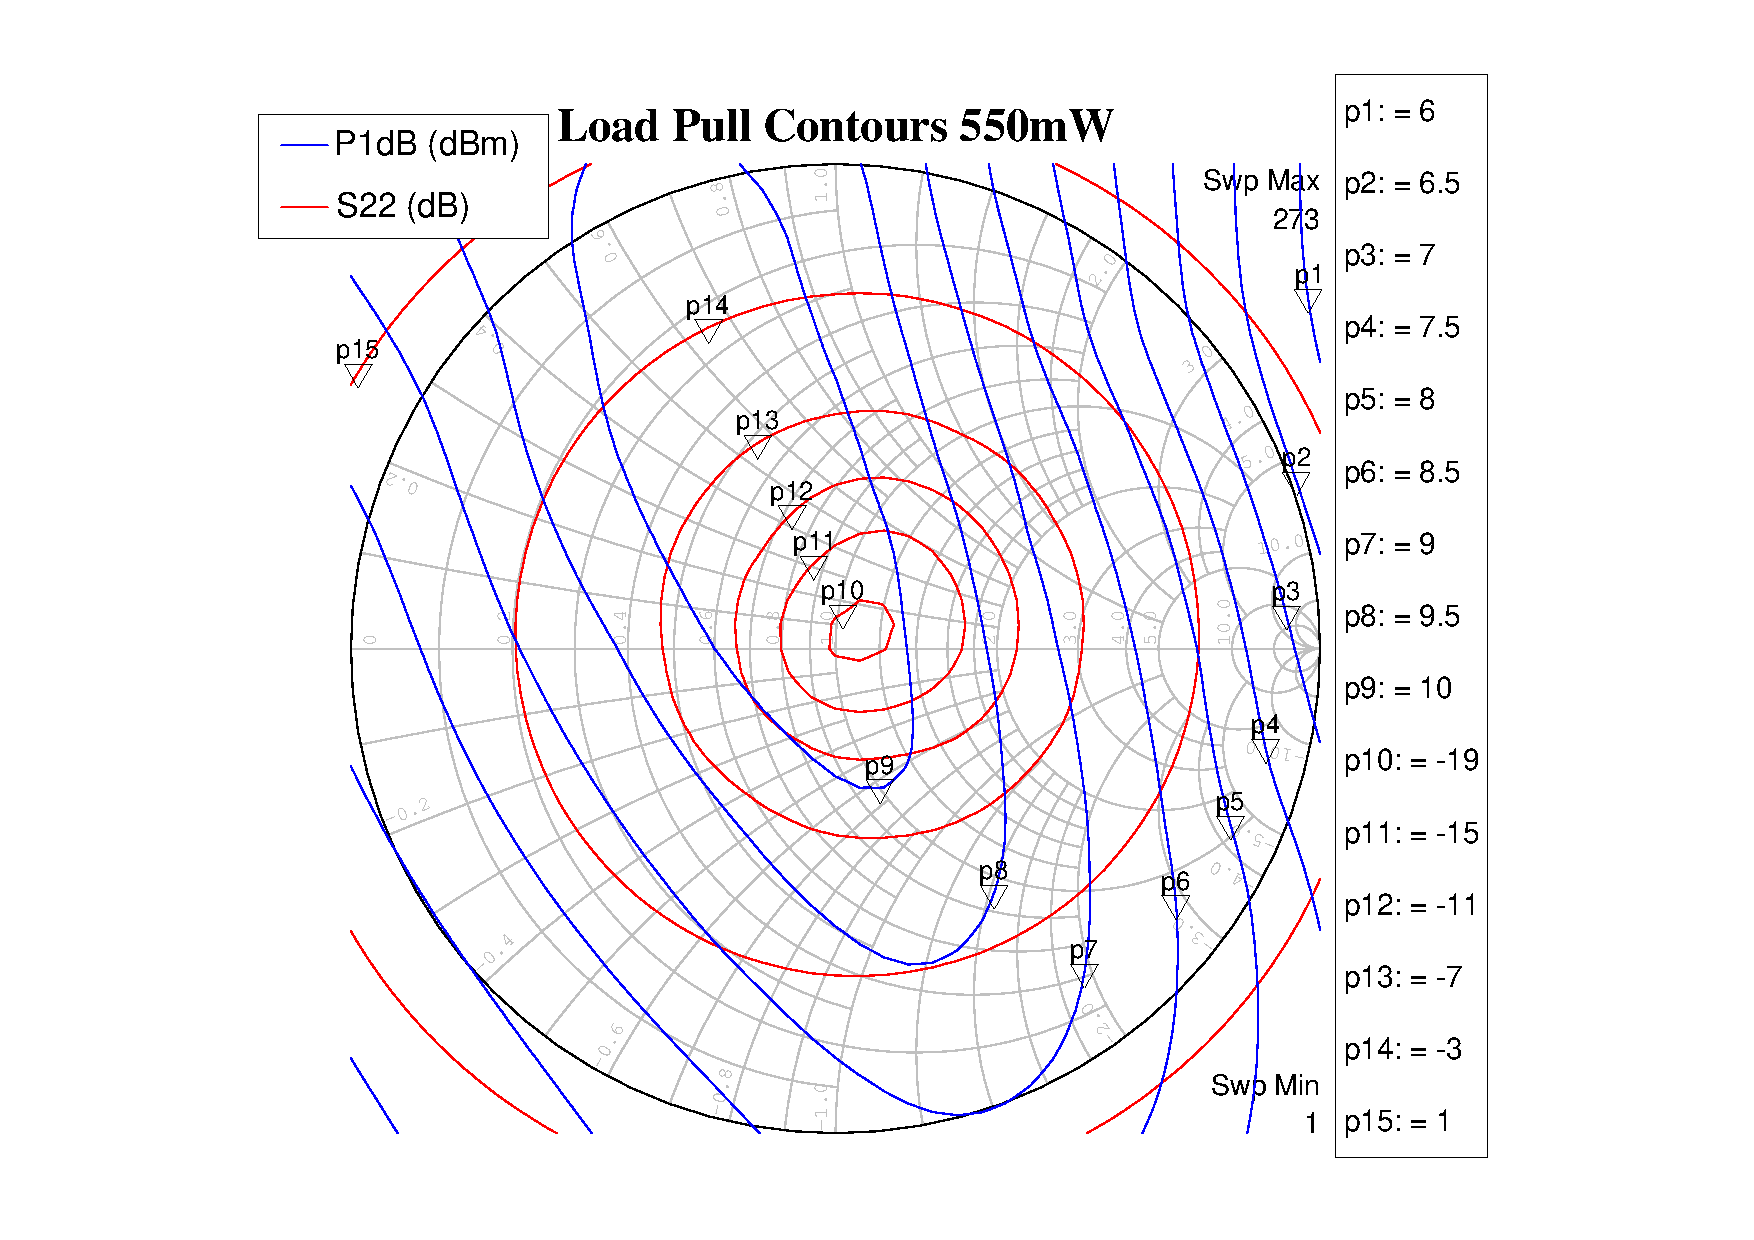
\includegraphics[trim=120 35 125 35, clip, width=0.7\textwidth]{fig/amplifiers/if2/loadpull550}
						\label{fig:if2lp550}
					}
					\caption[Load pull diagrams for IF amplifier 2.]{Load pull diagrams for optimal linearity (deformed contours) and optimal output matching (circular contours). The analysis is applied to a stable and matched amplifier with two \unit[6$\times$75]{\mum} FETs. The load pull diagrams show that devices biased in the most linear and high power region of the iv-curve (point C in \autoref{fig:fet_bias_point}) not only give a higher \unit[1]{dB} compression point overall but also a better match of the maximum $P_{1dB}$ with the optimal output impedance match.}\label{fig:if2lp}
				\end{figure}

		\subsection{Discussion}
			The thermal limitations force a two-FET amplifier design. This requires more space but effectively splits the source-drain current for each device in half. Another interesting observation is that the amplifier's linearity increased in the process. $P_{1dB}$ increased with \unit[4]{dB}, keeping the power consumption unchanged. The reason for this increase is attributed the same general reason why large devices are preferred over small when designing high-linearity class A amplifiers.

			Even though the junction temperature in the FETs has been reduced dramatically with the dual-FET design, the asymmetric design with only one source network causes a large current to flow through the upper transistor (\autoref{fig:if2layout}). The FET connected to the source has the DC-current of the other transistor in the source. In these UMS FETs, the source layers are connected with \unit[14]{\mum} air bridges. According to the maximum ratings these layers can only handle \unit[7.5]{mA/\mum}. This gives a total of $\unit[105]{mA}$ and the design is just above that ($\unit[110]{mA}$). The three alternatives are either to reduce the current $\unit[5]{mA}$, to widen the air bridge \unit[1]{\mum} or to route a common source for both FETs from the middle strip via an air bridge.

			The implemented negative parallel feedback provides wider bandwidth and easier matching. The bandwidth may seem unnecessary considering the narrow band. However, as amplifier IF1 is designed with a steep gain slope, it is preferable that this amplifier is not. This is due to the possibility of process variation in the frequency dependence. A variation within this design limits most damage in performance to amplifier IF1.

			The noise figure in the amplifier is approximately \unit[0.5]{dB} higher than in amplifier IF1. This shows that even though the input network is simpler, the parallel feedback results in an increase in noise. Also, no effort has been made to match noise optimum with the input match in this amplifier.



	\cleardoublepage
	\chapter{Variable attenuators}\label{ch:vargain}
	\section{Introduction}

		The IF-signal output should preferably be fixed in power as well as in frequency for later digital to analog-converters to be effective. In order to adjust the signal to a given level, the gain from the amplifiers is slightly higher than needed which, combined with variable attenuators, creates a variable gain circuit.

	
	%	It is specified that the variable gain should be controlled digitally, with \unit[3-4]{bits} of resolution and a gain of \unit[$\pm5$]{dB}, see \autoref{app:specs}. All attenuators are matched to \unit[50]{$\Omega$}. Bandwidth is not considered as the signal, after the mixer, has a narrow frequency band of \unit[20]{MHz} at \unit[2.14]{GHz}.  There are already variable attenuators implemented in PH25 and a comparison between basic attenuators in PPH25 concludes that there is little point in choosing another type.\autocite{gustavsson07}


	\section{Topologies}
		
		The simplest attenuator consists of a resistance that somehow interacts with the main RF line. Usually transistors are used to dynamically divert power into an attenuator, either into ground or back to the main line. This crude technique will however lead to relatively large reflections which is why slightly more sophisticated topologies are used. T- and $\Pi$-attenuators are common and offer small reflections, see Figures \ref{fig:tee_att_simple} and \ref{fig:pi_att_simple}.


		
		A fairly thorough discussion by \citeauthor{gustavsson07} concludes that due to compact size and ease of control, the T-structure makes the best choice of attenuator.\autocite{gustavsson07} The same arguments are valid for this circuit and process and thus the same type of attenuator is implemented. No notable differences are seen between PH25 and PPH25.

		\begin{figure}[ht]
			\begin{minipage}[b]{0.5\linewidth}
				\centering
				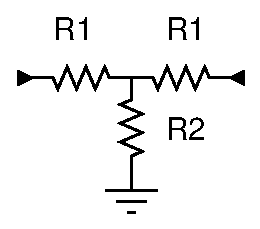
\includegraphics[width=0.5\textwidth]{fig/attenuators/tee-attenuator-symbolic}
				\caption{A tee-attenuator.}\label{fig:tee_att_simple}
			\end{minipage}
			\hspace{0.5cm}
			\begin{minipage}[b]{0.5\linewidth}
				\centering
				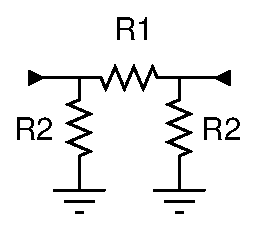
\includegraphics[width=0.5\textwidth]{fig/attenuators/pi-attenuator-symbolic}
			\caption{A pi-attenuator.}\label{fig:pi_att_simple}
			\end{minipage}
		\end{figure}

	\section{Design}

		The values of the resistances $R_1$ and $R_2$ for the T-attenuator are given as \autocite{matthaei80}
		\begin{align*}
			R_1 &= Z_0 \left[\frac{10^{A/20}-1}{10^{A/20}+1}\right] \\
			R_2 &= 2Z_0 \left[\frac{10^{A/20}}{10^{A/10}-1}\right]
		\end{align*}
		In order to control the attenuator, two FET's are added between the tee-pad and ground and in parallel with the tee-pad, see \autoref{fig:tee_att_symbolic}. When V1 is closed and V2 open, there is no attenuation. Opening V1 and closing V2 forces the current to go through the resistances and partly into ground resulting in an attenuation.

		The attenuators are  biased by giving the source \unit[+5]{V} and switching  the gate voltage between \unit[3]{V} and \unit[5]{V}. Therefore a DC-block must be added between V2 and ground in \autoref{fig:tee_att_symbolic}. 
		
		\begin{figure}[h!]
			\centering
			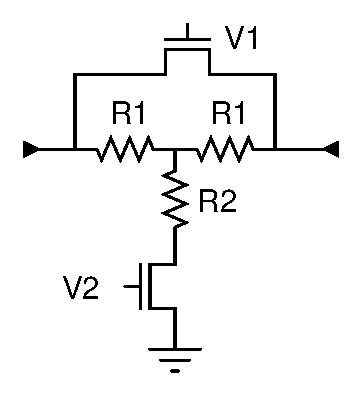
\includegraphics[width=0.4\textwidth]{fig/attenuators/tee-attenuator-variable-symbolic}
			\caption[A tee-attenuator schematically]{A tee-attenuator schematically. By switching the FETs, the gain is changed. When V1 is shorted and V2 open, the attenuator is not active. By reversing the voltages, the attenuator is activated.}\label{fig:tee_att_symbolic}
		\end{figure}



		The values of $R_1$ and $R_2$ are optimized to account for the extra capacitor and FET parasitics. The gates of the FETs are connected via high-value resistors to the control blocks. The high-value resistors are added to increase the FET's $S_{21}$ in its closed state, see \autoref{fig:fet_gate_resistance}. A \unit[6]{k$\Omega$} resistance is chosen, as in the PH25-process. 

		

		\begin{figure}[h!]
			\centering
			\includerect{0.7\textwidth}{fig/fet_gate_resistance}
			\caption[Drain-source conductance depending on gate impedance.]{The inherent attenuation of the FET in its closed state, depending on gate impedance for the switching FET  (PPH25SSW).}\label{fig:fet_gate_resistance}
		\end{figure}		
		
		\begin{figure}[h!]
			\centering
			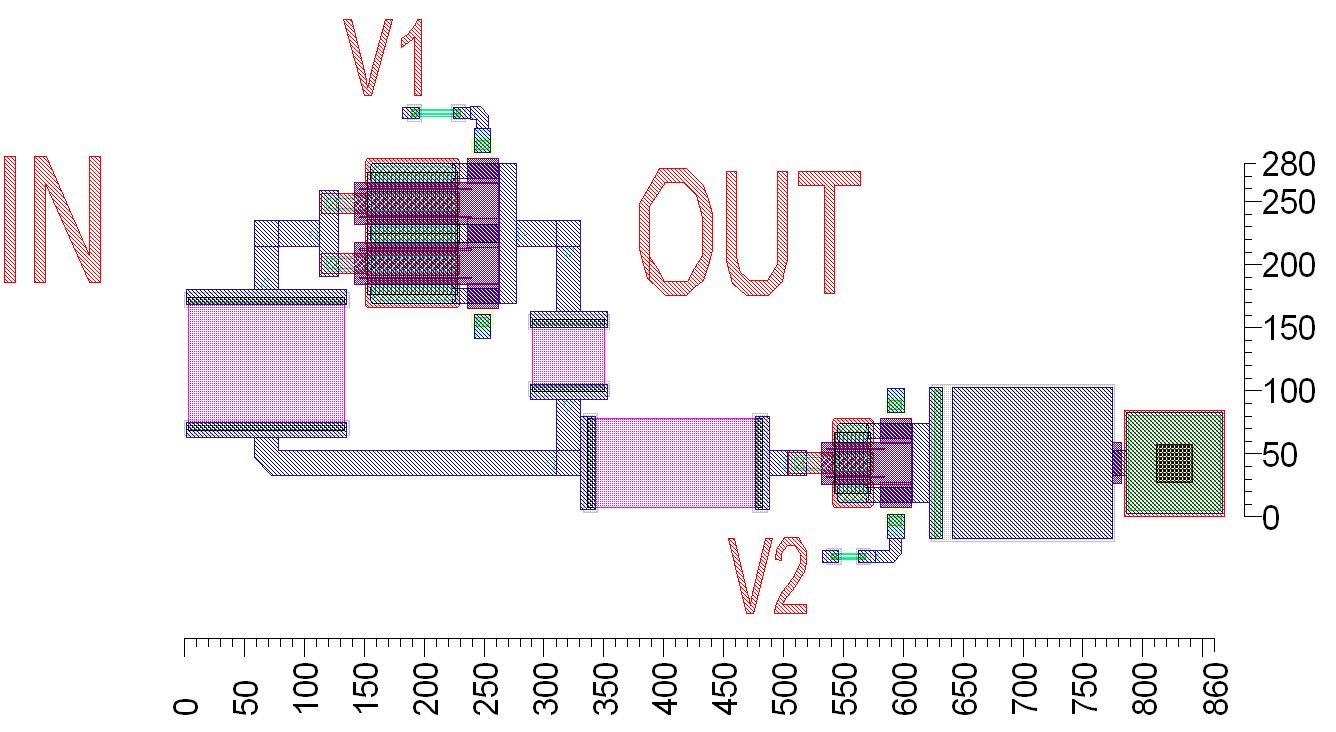
\includegraphics[width=1.0\textwidth]{fig/attenuators/tee_att_layout_6dB}
			\caption[Layout of a tee-attenuator]{Layout of the 6dB-attenuator.  A high-value resistor is connected to the gate of the FETs.\scalemum}\label{fig:tee_att_layout}
		\end{figure}
		
		%6dB att: Max 40mA on $R_0$ and 22mA over $R_1$ when sending 16dBm across. With 0.4mA/\mum, the width has to be 100 and 55 respectively.
		% I0, I0, I1 => W0, W0b, W1
		%6dB: 53, 25, 28mA
		%3dB: 60mA, 43, 18mA => 150, 110, 45
		%1.5dB: 45mA, 40mA, 6mA => 110, 100, 15
		
			

	\section{Combining attenuators}

		Several techniques are available when combining attenuators to achieve a spectrum of discrete points. Attenuators can be connected in parallel or in series. A parallel connection results in a smaller total loss when all attenuators are inactive, i.e. when maximum gain is sought. This is because of the inherent drain-source resistance in the transistors used for overriding the attenuators. When connecting attenuators in parallel, the total loss is smaller in their inactive state but there are fewer possible states of attenuation.

		As maximizing the number of controlling bits and thereby saving chip-size is deemed important, it is decided to use a series design of the attenuators. Furthermore, a resolution of \unit[1.5]{dB} and a total of \unit[3]{bits} suffices. This gives $2^3=8$ steps and a maximum attenuation of $1.5+3+6=\unit[10.5]{dB}$.

%		If the free chip-space allows it in the end, one possibility may be to add an additional \unit[0.8]{dB} attenuator. %TODO at end of project, is this still valid?

The entire attenuator-circuit must be properly biased. Therefore there are DC-blocks before and after the attenuators. The entire line is raised to \unit[+5]{V} by connecting the bias-voltage through a high-resistance element serving as IF-block (\autoref{fig:attenuator-chain-symbolic}).

		\begin{figure}[h!]
			\centering
			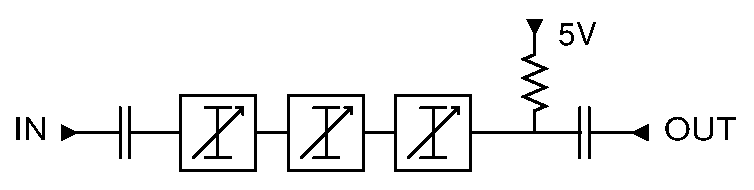
\includegraphics[width=0.8\textwidth]{fig/attenuators/attenuator-chain-symbolic}
			\caption[The attenuator-circuit schematically]{The three attenuators with DC-blocks raised to \unit[5]{V} so that the FETs are properly biased. The attenuators are controlled by level-shifters as explained in the following chapter.}\label{fig:attenuator-chain-symbolic}
		\end{figure}

	
	\section{Results}
		
		When simulating the attenuators, there is the option of using a linear model of the switching FET called PPH25SSW or the non-linear cold FET called PPH25NCF. The non-linear models are more powerful in that they can be used in non-linear simulations but the linear switching FET  models approximate linear operation better. The simulations are performed with PPH25SSW as far as possible.		
		
		The attenuation values and reflection coefficients for all attenuators are displayed in \autoref{tab:VarGainData}. All attenuation states, including spread are seen in \autoref{fig:All_attenuators_spread}. The compression point, $P_{1dB}$, for the complete variable-gain-circuit (three attenuators in series) is calculated to \unit[22]{dB} using PPH25NCF when all attenuators are in their inactive state. All other states result in higher $P_{1dB}$.
	
	
	
		\begin{table}[h!]
			\caption{Simulated attenuator data for PPH25SSW.}
			\label{tab:VarGainData}
			\centering
			\begin{tabular}{ l l l l } \toprule
				Attenuator & 	$S_{21,\text{diff}}$ &	$S_{21,\text{off}}$ &  $S_{11}$, $S_{22}$ \\\midrule
				\unit[1.5]{dB} & \unit[1.5]{dB}	&	\unit[0.36]{dB} & $>$\unit[25]{dB} \\
				\unit[3]{dB} & \unit[3.0]{dB}	&	\unit[0.34]{dB} & $>$\unit[25]{dB} \\
				\unit[6]{dB} & \unit[6.1]{dB}	&	\unit[0.35]{dB} & $>$\unit[21]{dB} \\\bottomrule
			\end{tabular}
		\end{table}


%		\begin{figure}[hbt!]
%			\centering
%			\includerect{1.0\textwidth}{fig/attenuators/S_params_1_5dB}
%			\caption[The S-parameters of the 1.5dB attenuator]{The S-parameters of the 1.5dB attenuator with switching FET. Spread is included as a TiWiSi-resistor is used which has a large spread.}\label{fig:S_params_1_5dB}
%		\end{figure}

%		\begin{figure}[hbt!]
%			\centering
%			\includerect{1.0\textwidth}{fig/attenuators/S_params_3dB}
%			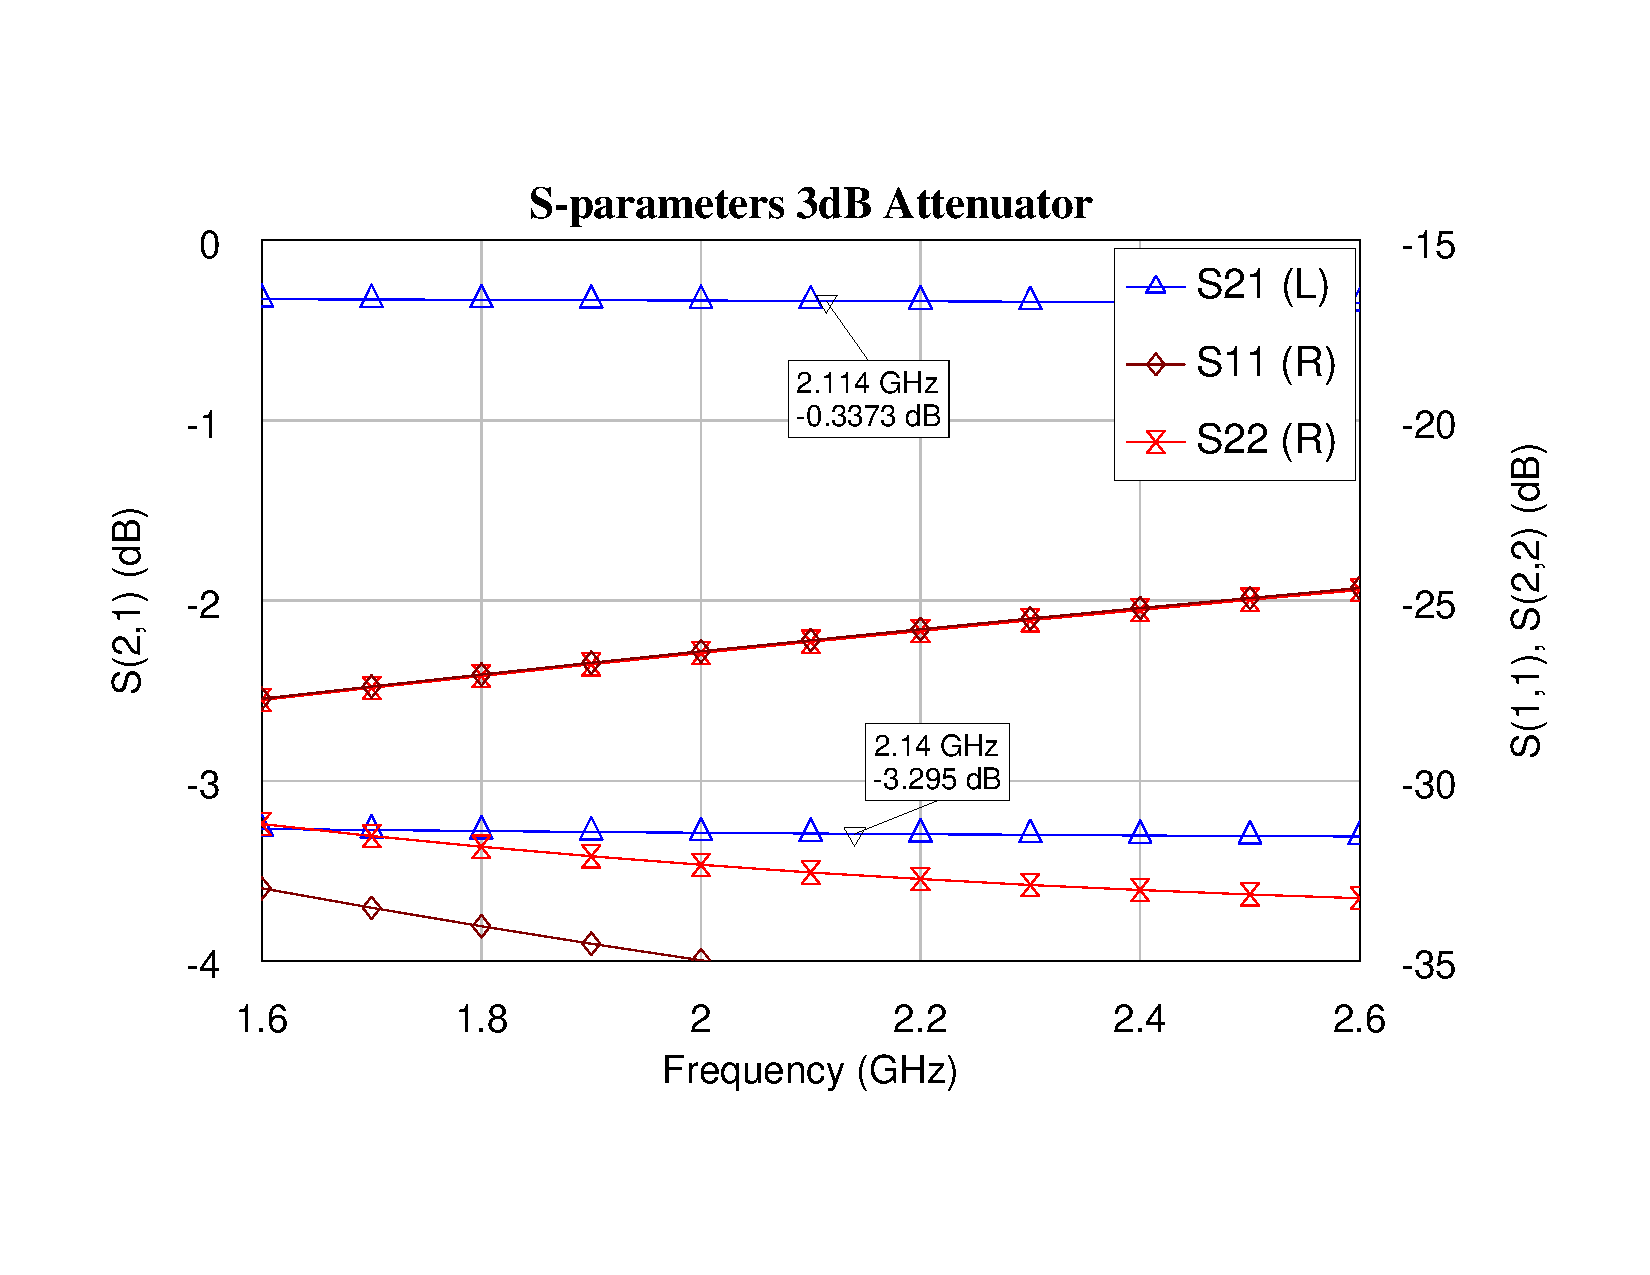
\includegraphics[width=1.0\textwidth]{fig/attenuators/S_params_3dB}
%			\caption[The S-parameters of the 3dB attenuator]{The S-parameters of the 3dB attenuator with PPH25SSW}\label{fig:S_params_3dB}
%		\end{figure}


		\begin{figure}[h!]
			\centering
			\includerect{1.0\textwidth}{fig/attenuators/All_attenuators_spread}
			\caption[Spread for all gain-states]{Spread for all gain states using PPH25SSW.}\label{fig:All_attenuators_spread}
		\end{figure}


		
		%In \autoref{fig:P1dB_Complete}, 
		

%		\begin{figure}[hbt!]
%			\centering
%			\includerect{1.0\textwidth}{fig/attenuators/P1dB_Complete}	
%			\caption[$P_{1dB}$ for entire attenuator-circuit]{Output power as a function of input power for  the complete attenuator-circuit. Shows the $P_{1dB}$-point.  All dampeners are in their inactive state, other states results in higher $P_{1db}$. Using PPH25NCF.}\label{fig:P1dB_Complete}
%		\end{figure}

		\begin{figure}[h!]
			\centering
			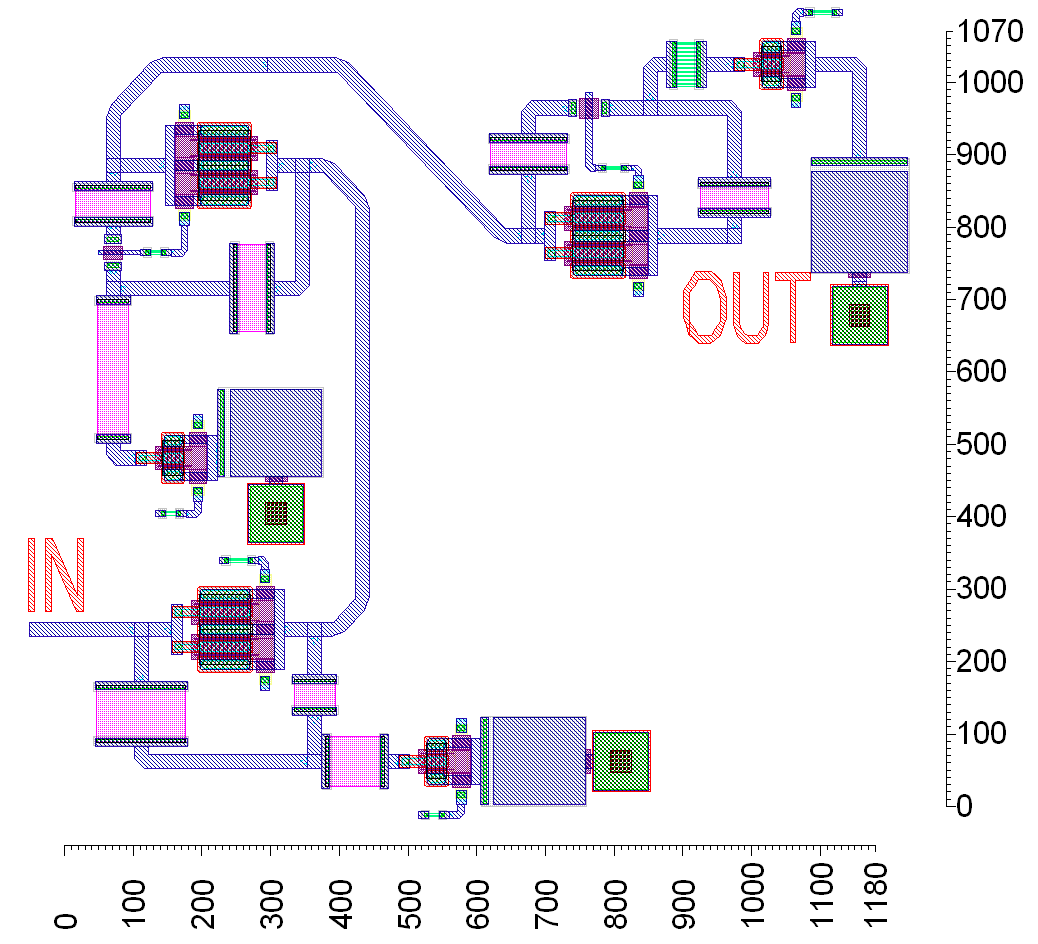
\includegraphics[width=0.8\textwidth]{fig/attenuators/attenuators_layout}
			\caption[Attenuator circuit layout]{The complete attenuator circuit.\scalemum}\label{fig:attenuators_layout}.
		\end{figure}

	
				


		
		%\begin{figure}[hbt!]
		%	\centering
		%	\includegraphics[width=1.0\textwidth]{fig/attenuators/All_attenuators}
		%	\caption{The complete attenuator circuit.}\label{fig:P1dB_Complete}
		%\end{figure}

%%%%%%%%%%%%%%%%%%%%%%%%%%%%%%%%%%%%%%%%%%%%%%%%%%%%%%%%%%%%%%%%%%%%%%%%%%%%%%%%%%%%%%%%%%%%%%%%%%%%%%%%%%%%%%%%%%%%%%%%%%%%%%%%%%
%%%%%%%%%%%%%%%%%%%%%%%%%%%%%%%%%%%%%%%%%%%%%%%%%%%%%%%%%%%%%%%%%%%%%%%%%%%%%%%%%%%%%%%%%%%%%%%%%%%%%%%%%%%%%%%%%%%%%%%%%%%%%%%%%%
\section{Attenuator control}

	\subsection{Introduction}
		The attenuators are controlled by applying either \unit[5]{V} or \unit[3]{V} to the FET's gates, thereby switching them between completely on and completely off. This is the task of the so called level shifters. The level shifters take as input a binary zero (\unit[0-.4]{V}) or one (\unit[1.8-5]{V}), adhering to the standardized LvTTL-logic.\autocite{lvttl11} % Double check these values for pph225
		
		This technique is well established at SAAB and there are existing models for the PH25-process\autocite{gustavsson07}. The level shifters are implemented again in PPH25 without any major changes.
		
	\subsection{Design}
		The schematic  and real layout for the level shifter are seen in \autoref{fig:level_shifter_sch} and \autoref{fig:level_shifter_layout}, respectively.
		In short, $v_{control}$  directly controls $T1$. When $T1$ is closed, $v_1=\unit[3]{V}$ as the bias voltage will split over $R_2$ and $R_6$. This in turn will cause $T_2$ to open, making  $v_2=\unit[5]{V}$. As $v_{control}$ is decreased, $T_1$ will eventually open, making $v_1=\unit[5]{V}$. As there will no longer be any current over $R_6$, $v_{gs}$ over $T_2$ will decrease, and $T_2$ will close, making $v_2=\unit[3]{V}$.
		
		The level shifter's output is shown in Figure\autoref{fig:levelshifter_output_spread}. By adjusting the two resistances between $V_{control}$ and ground in the circuit, the voltage at which the attenuator is turned on, $V_{shift}$ is adjusted. Also, the current consumption can be decreased by increasing the remaining resistances. However, there comes the penalty in the form of increased size. See Figure\autoref{fig:levelshifter_current} for the current consumption.


		\begin{figure}[h!]
			\centering
			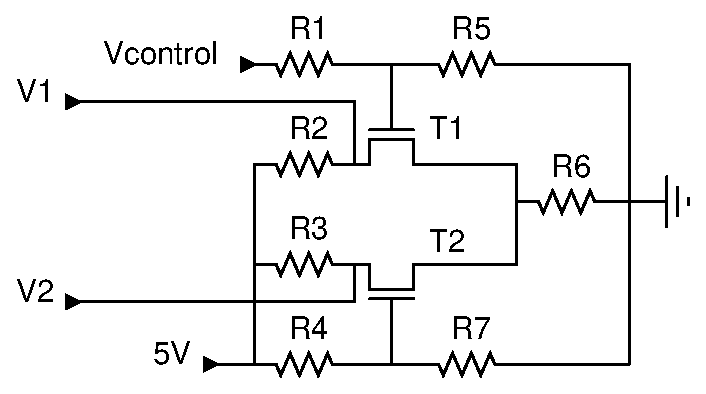
\includegraphics[width=0.7\textwidth]{fig/attenuators/sch_level_shifter}
			\caption[Level-shifter schematic layout]{Schematic of the level-shifter used for biasing the attenuators. $T_1,T_2$=\unit[1$\times$25]{\mum}, $R_1=\unit[1.0]{k\Omega}$, $R_2=\unit[2.1]{k\Omega}$, $R_3=\unit[3.3]{k\Omega}$, $R_4=\unit[20]{k\Omega}$, $R_5=\unit[6.2]{k\Omega}$, $R_6=\unit[3.0]{k\Omega}$ and $R_7=\unit[5.0]{k\Omega}$.}\label{fig:level_shifter_sch}
		\end{figure}
		
		
		\begin{figure}[h!]
			\centering
			\includegraphics[width=1.0\textwidth]{fig/attenuators/level_shifter_layout}
			\caption[Level shifter layout]{The layout on-chip for the level shifter used for biasing the attenuators.}\label{fig:level_shifter_layout}
		\end{figure}


	\begin{figure}[h!]
			\centering 
			\subfloat[][Level shifter output with yield analysis.]{
				\includerect{0.5\textwidth}{fig/attenuators/level_shifter_output_spread}
				\label{fig:levelshifter_output_spread}
			}
			\subfloat[][Level shifter current consumption with yield analysis.]{
				\includerect{0.5\textwidth}{fig/attenuators/level_shifter_current}
				\label{fig:levelshifter_current}
			} 
			\caption[Level shifter output]{\subref{fig:levelshifter_output_spread} Voltages generated by the level shifter and \subref{fig:levelshifter_current} current consumption as a function of the control signal.}\label{fig:level_shifter_data}
		\end{figure}

		
%		\begin{figure}[hbt!]
%			\centering
%			\includerect{1.0\textwidth}{fig/attenuators/level_shifter_output_spread}
%			\caption[Level shifter output]{The voltages generated by the level shifter as a function of the control signal. Spread analysis is applied.}\label{fig:level_shifter_current}
%		\end{figure}
		


%		\begin{figure}[hbt!]
%			\centering
%			\includerect{1.0\textwidth}{fig/attenuators/level_shifter_current}
%			\caption[Level shifter current use]{The current consumption of the level shifter for different control signals.}\label{fig:level_shifter_current}
%		\end{figure}





	\settocdepth{subsection}
	\cleardoublepage
	\chapter{Chip Summary And Final Conclusions}
	
		The complete circuit design is the final product of this work. It is based on the three previous chapters explaining the design of the chip's individual components. This chapter explains the final layout with connecting pads and lists the final full-chip simulations. The chip is compared to design specifications and potential improvements are discussed. The report is wrapped up with some final conclusions.
		
		%The complete chip-performance has been simulated, both with EM-models of each sub-circuit and for s
		%

	\section{Layout}
		The complete chip is designed to fit into a \unit[4$\times$5]{mm} QFN-package (\autoref{fig:final_chip}). The chip components are placed according to a few requirements:

		First of all, the incoming RF- and outgoing IF-port should ideally be placed on opposite sides of the chip. In order to avoid interference, it would be preferable to have the LO-port on one of the remaining sides. Early on, a straight signal path was favored over more complex choices although this wasn't really a requirement and was relaxed as the chip-layout matured. %The size of the chip had to be \unit[2.4x3.4]{mm} as a smaller

		The diplexer is a big sub-circuit and rather significant to the entire chip-function and at large decides the placement of other circuits on the chip. The LO-amplifier is quite small and connects straight to the mixer. The remaining subcircuits: Two IF-amplifiers and three attenuators are adjusted to fit together.

		The final layout has the RF-port and IF-port on opposite short sides of the chip coupled with ground-pads. No other pads are placed on the short sides to keep the bonding wires isolated. The LO-signal and two bias-signals for the mixer and LO-amplifier respectively are connected on one of the long sides. The bias-signals for the two circuits are separated and isolated with two grounded pads. This gives the possibility of biasing the mixer and/or the amplifier with signals different from \unit[5]{V} in the future.
	
		On the remaining long side, three \unit[5]{V} bias-signals for the IF1-, IF2-amplifiers and the attenuator-circuit enters, as well as three control-signals for the attenuators.
		
		Grounded pads are placed next to the major bias-pads. They are put there in order to make accurate measurements of the naked chip. These pads are however not connected to exterior bonding pads for the packaged chip.

		\begin{figure}[hbt!]
			\centering
			\includegraphics[width=1.0\textwidth]{fig/summary/package}
			\caption[Layout of the pad-structure.]{Layout of the MMIC and labels of the bonding pads. The size of the final package is \unit[4$\times$5]{mm}. The effective chip area containing all components is \unit[2.3$\times$3.3]{mm}. C1, C2 and C3 provide the control signals for the \unit[6]{dB}, \unit[3]{dB} and \unit[1.5]{dB} attenuators respectively.}\label{fig:final_chip}
		\end{figure}

	\section{Performance}
		\subsection{Summary}
			Summary of simulated chip performance at nominal gain (\autoref{tab:chipsummary_nominal}), maximum gain (\autoref{tab:chipsummary_maximum}) and minimum gain (\autoref{tab:chipsummary_minimum}).
			
			\begin{table}[hbt!]
				\caption[Summarized chip performance at nominal gain.]{Summary of chip performance at nominal gain. LO drive at \unit[-2]{dBm}.\disclaimer}
				\label{tab:chipsummary_nominal}
				\centering
				\begin{tabular}{ l c c c c c c l } \toprule
					Parameter & Min. & Typ. & Max. & Min. & Typ. & Max. & Unit \\\midrule
					Frequency range RF & \multicolumn{3}{c}{2.9--3.4} & \multicolumn{3}{c}{3.1--3.3} & GHz \\
					Frequency range LO & \multicolumn{3}{c}{5.04--5.54} & \multicolumn{3}{c}{5.24--5.44} & GHz \\
					Frequency IF & \multicolumn{3}{c}{2.14} & \multicolumn{3}{c}{2.14} & GHz \\
					Return loss RF & 14 & 16 &  & 20 & 21 &  & dB \\
					Return loss LO & 13.5 & 17 &  & 17 & 18 &  & dB \\
					Return loss IF & 23 & 24 &  & 23 & 24 &  & dB \\
					Conversion gain & 10.3 & 10.6 & 10.8 & 10.7 & 10.8 & 10.8 & dB \\
					Gain variation & & 0.45 & 0.45 & & 0.05 & 0.05 & dB \\
					Image rejection & 48 & 50 &  & 50 & 51 &  &  dB \\
					$P_{1dB}$ (input) & 9.8 & 10.0 &  & 9.8 & 10.0 &  & dBm \\
					$IIP_3$ (estimate) & 20 & 20 &  & 20 & 20 &  & dBm \\
					Noise figure (estimate) &  & 11 & 11 &  & 11 & 11 & dB \\
					Power consumption &  & 1.0 & 1.0 &  & 1.0 & 1.0 & W \\\bottomrule
				\end{tabular}
			\end{table}
			
			\begin{table}[hbt!]
				\caption[Summarized chip performance at maximum gain.]{Summary of chip performance at maximum gain (\unit[+4.5]{dB}). Only parameters which performance has changed compared to the case with nominal gain are presented. LO drive at \unit[-2]{dBm}.\disclaimer}
				\label{tab:chipsummary_maximum}
				\centering
				\begin{tabular}{ l c c c c c c l } \toprule
					Parameter & Min. & Typ. & Max. & Min. & Typ. & Max. & Unit \\\midrule
					Frequency range RF & \multicolumn{3}{c}{2.9--3.4} & \multicolumn{3}{c}{3.1--3.3} & GHz \\
					Return loss IF & 29 & 31 &  & 29 & 31 &  & dB \\
					Conversion gain & 14.7 & 15.0 & 15.2 & 15.1 & 15.2 & 15.2 & dB \\
					$P_{1dB}$ (input) & 6.6 & 6.7 &  & 6.6 & 6.7 &  & dBm \\
					$IIP_3$ (estimate) & 17 & 17 &  & 17 & 17 &  & dBm \\
					Noise figure (estimate) &  & 10 & 10 &  & 10 & 10 & dB \\\bottomrule
				\end{tabular}
			\end{table}
			
			\begin{table}[hbt!]
				\caption[Summarized chip performance at minimum gain.]{Summary of chip performance at minimum gain (\unit[-6.0]{dB}). Only parameters which performance has changed compared to the case with nominal gain are presented. LO drive at \unit[-2]{dBm}.\disclaimer}
				\label{tab:chipsummary_minimum}
				\centering
				\begin{tabular}{ l c c c c c c l } \toprule
					Parameter & Min. & Typ. & Max. & Min. & Typ. & Max. & Unit \\\midrule
					Frequency range RF & \multicolumn{3}{c}{2.9--3.4} & \multicolumn{3}{c}{3.1--3.3} & GHz \\
					Return loss IF & 21 & 22 &  & 21 & 22 &  & dB \\
					Conversion gain & 4.3 & 4.6 & 4.8 & 4.7 & 4.8 & 4.8 & dB \\
					$P_{1dB}$ (input) & 11.3 & 11.5 &  & 11.3 & 11.5 &  & dBm \\
					$IIP_3$ (estimate) & 21 & 21 &  & 21 & 21 &  & dBm \\
					Noise figure (estimate) &  & 13 & 13 &  & 13 & 13 & dB \\\bottomrule
				\end{tabular}
			\end{table}
			
		\subsection{Return loss}
			The return losses at the RF- and LO-ports are simulated and found to be very similar as those simulated for the individual components. The results are listed in the chip summary but for detailed frequency characteristics see \autoref{fig:mixermatch} for the RF-port and \autoref{fig:lo_reflections} for the LO-port. The IF-port's return loss depends on the gain setting and is found to be at least \unit[21]{dB} in all cases with a \unit[100]{MHz} bandwidth.
			
		\subsection{Conversion gain}
			The chip's conversion gain is simulated for all gain states in \autoref{fig:sysgainstates} and for different LO drives in \autoref{fig:sysgainvslo}.
			
			\begin{figure}[hbt!]
				\centering
				\includerect{0.8\textwidth}{fig/summary/gainvsstate}
				\caption[Chip gain for all gain states.]{Chip gain versus frequency for all gain states. $P_{lo}=\unit[-2]{dBm}$. The least significant bit (LSB) is \unit[1.55]{dB} and the dynamic gain is \unit[10.3]{dB}.}\label{fig:sysgainstates}
			\end{figure}
			
			\begin{figure}[hbt!]
				\centering
				\includerect{0.8\textwidth}{fig/summary/gainvslo}
				\caption[Chip gain for different LO drives.]{Chip gain versus frequency for different LO drives at nominal gain. The gain variation is kept below \unit[0.6]{dB} between \unit[2.9 and 3.4]{GHz} for $P_{lo}$=\unit[-4 to 0]{dBm}.}\label{fig:sysgainvslo}
			\end{figure}
			
			The IF signal has a narrow bandwidth. Even so, the \unit[20]{MHz} on the MMIC that it does occupy exhibits a frequency dependent gain according to \autoref{fig:ifbehave}. This plot is also interesting, should the frequency characteristics in the IF-path shift.
			
			\begin{figure}[hbt!]
				\centering
				\includerect{0.8\textwidth}{fig/summary/ifbehave}
				\caption[IF-frequency dependent chip gain.]{IF-frequency dependent chip gain. The gain variation in the \unit[20]{MHz} wide IF band is \unit[0.2]{dB}}\label{fig:ifbehave}
			\end{figure}
			
		\subsection{Linearity}
			Chip $P_{1dB}$ for different gain states and LO drives are plotted in \autoref{fig:sysp1db}. The linearity is as expected highest for minimum gain and lowest for maximum gain. $P_{1dB}$ tends to drop for smaller LO-drives. 
			
%			\begin{figure}[hbt!]
%				\centering
%				\includerect{0.8\textwidth}{fig/summary/chipcompression}
%				\caption[Chip gain compression.]{Chip gain compression at different gain states and for different LO input powers. Traces with $\triangle$ are measured at maximum gain, $\medsquare$ at nominal gain and $\diamond$ at minimum gain. The LO powers range between \unit[-4 and 0]{dBm}. Compression occurs earlier for higher gain. The results are summarized using $P_{1dB}$ in \autoref{fig:sysp1db}.}\label{fig:syscompression}
%			\end{figure}
			
			\begin{figure}[hbt!]
				\centering
				\includegraphics[width=0.8\textwidth]{fig/summary/chipp1db}
				\caption[Chip $P_{1dB}$.]{Chip $P_{1dB}$ for different gain states versus input LO power.}\label{fig:sysp1db}
			\end{figure}
			
		\subsection{Spectrum and spurious frequencies}
			The frequency spectrum from \unit[0 to 10]{GHz} at the output IF port is shown in \autoref{fig:sysspectrum}.
			
			\begin{figure}[hbt!]
				\centering
				\includerect{1.0\textwidth}{fig/summary/spectrum}
				\caption[IF-port output spectrum.]{Frequency spectrum at the output IF-port for input frequency \unit[3.2]{GHz}, $P_{lo}=\unit[-2]{dBm}$ and nominal gain. Noteworthy components are: IF (\unit[2.14]{GHz}), RF (\unit[3.2]{GHz}), LO (\unit[5.34]{GHz}), 2$\times$IF (\unit[4.28]{GHz}), RF-IF (\unit[1.06]{GHz}) and RF+IF (\unit[8.54]{GHz}). The LO isolation is \unit[21]{dB}, which is just above the required level of \unit[20]{dB}. The 2$\times$IF-signal suppression is \unit[38]{dBc}, which is \unit[2]{dB} below the required value. The RF-signal has only \unit[7.6]{dB} isolation. Some of the smaller components are spurious frequencies predicted in \autoref{tab:introsingletone}.}\label{fig:sysspectrum}
			\end{figure}
			

			
		\subsection{Maximum rating}
			All the components are scaled to survive a maximum input power level of $P_{RF}=\unit[17]{dBm}$. This is the maximum power the circuit prior to this mixer chip is able to deliver. The major concerns are the resistors' widths and the width of the microstrips. The sizes are scaled according to UMS specifications.\autocite{pph25manual}
			
			Transistors may not survive if the junction temperature becomes too high. The FETs in the IF-amplifiers run the risk of overheating due to their large current consumption. They are designed to survive a maximum chip backside temperature of \unit[100]{$^\circ$C} which is thought possible in the event of starting the system in a warm dessert for example.
			
	
	\section{Temperature and yield analysis}	
		\subsection{Components}
			Components are affected by temperature as well as production spread. An analysis of the chip performance for different temperatures and yields has been performed. The chip is required to keep its performance between \unit[-40]{$^\circ$C} and \unit[55]{$^\circ$C} and to function up to \unit[85]{$^\circ$C}. 			
			
			The temperature dependence arise mostly in the TiWSi- and GaAs-resistors where the resistance differs $\sim$\unit[10]{\%} as temperature goes from \unit[20]{$^\circ$C} to \unit[85]{$^\circ$C}. The FETs have a temperature dependence as well but the PPH25 models only allow simulations at \unit[20]{$^\circ$C}. Some qualitative arguments can be made by reviewing PH25 FET performance. The gain in PH25 FETs have approximately a \unit[-0.2]{$\%$/K} dependence and this is believed to hold for PPH25 as well considering how similar the processes are. This gives an extra gain of \unit[0.5]{dB} at \unit[-40]{$^\circ$C} and decreases the gain of each FET with \unit[0.25]{dB} at \unit[55]{$^\circ$C}.		

		\subsection{Conversion gain}
			The entire chip's conversion gain is simulated for temperatures between \unit[-40]{$^\circ$C} and \unit[85]{$^\circ$C} (\autoref{tab:chip_temperature_dependence}). The conversion gain increases slightly as temperature increases to \unit[85]{$^\circ$C}. It is believed that the unaccounted temperature dependence of the FET's gain has a reverse effect on the increased chip gain. %Using data from PH25, a FET's gain drops approximately \unit[0.5]{dB} as temperature goes from \unit[20 to 85]{$^\circ$C}. % 60*(-0.2) = -12% gain at 85C. Which gives 10*log(1-60*0.002) = -0.5dB

			
		By taking temperature, yield and the FET's temperature dependence into account, the minimum and maximum chip conversion gain is \unit[9.4]{dB} at \unit[55]{$^\circ$C} and \unit[12]{dB} at \unit[-40]{$^\circ$C}, respectively. This is at the nominal gain state.


		\begin{table}[h!]
				\caption[Chip conversion gain temperature dependence]{Chip conversion gain with yield analysis at nominal gain. The simulation is performed with circuit models where the resistors are adjusted for temperature. PPH25 FET models can only be simulated at \unit[20]{$^\circ$C} and the decreased gain of the FETs at higher temperatures is therefore not included.}
				\label{tab:chip_temperature_dependence}
				\centering
				\begin{tabular}{ l c } \toprule % Circuit simulation gain: 2.6 3.2, 3.5, 3.9
					Temperature & Conversion gain \\\midrule
					\unit[-40]{$^\circ$C} 	& $\unit[10.0\pm1]{dB}$\\
					\unit[20]{$^\circ$C} 	& $\unit[10.6\pm1]{dB}$\\
					\unit[55]{$^\circ$C} 	& $\unit[10.9\pm1]{dB}$ \\
					\unit[85]{$^\circ$C}	& $\unit[11.3\pm1]{dB}$ \\\bottomrule
				\end{tabular}
			\end{table}			
	

		\subsection{Compression point}
		The \unit[1]{dB}-compression point could not be successfully simulated using circuit-models and therefore a qualitative argument must be made using performance of subcircuits and theory.
		
		Since the gain of the FETs decrease with temperature, it can be argued that the IF-amplifiers' compression-points will not decrease at higher temperatures. The LO-amplifier loses \unit[0.4]{dB} of gain at \unit[55]{$^\circ$C} due to its TiWSi-feedback loop and reduced FET-gain which may affect the mixer $P_{1dB}$ with as much. This does not affect the chip compression point by more than \unit[-0.1]{dB} at nominal gain. It is therefore probable that higher temperatures will not affect the chip compression point more than \unit[-0.1]{dB}. 
		
		At temperatures close to \unit[-40]{$^\circ$C}, the gain of each FET increases with \unit[0.5]{dB}. As a side effect, the IF-amplifiers' compression-points decrease with \unit[0.5]{dB} which decreases the chip compression point with \unit[-0.2]{dB} according to the cascade formulas, \autoref{eq:casciip3}. The positive effect of having a larger LO drive is unaccounted for.	This analytical approach results in the chip's compression point being rather temperature-invariant. The yield analysis shows a smallest mixer $P_{1dB}$ of \unit[10]{dB} at $P_{lo}=\unit[-4]{dBm}$. With a \unit[0.5]{dB} and \unit[0.5]{dB} decrease in $P_{1dB}$ for the IF-amplifiers respectively, the effect on the chip's \unit[1]{dB}-compression point is a decrease of \unit[1]{dB} at nominal gain.
		
		By using the yield analysis of sub-circuits and an analytical temperature analysis, the chip $P_{1dB}$ is believed to lose \unit[$\sim$1]{dB} at \unit[-40]{$^\circ$C}.

	
	\section{Discussion}
		\subsection{Comparison to design specifications}
			In Tables \ref{tab:syscomparisonnarrow} and \ref{tab:syscomparisonbroad} is a comparison between design specifications and the simulated chip performance shown. The nominal gain is approximately \unit[1]{dB} higher than specified. This is acceptable, considering that the dynamic gain range is \unit[10.5]{dB} and that the gain empirically is lower than simulated.
			
%			\ctable[ caption = Achieved performance compared to design specifications. For many parameters there is no target specification and the entry is left blank. As chip performance varies a lot with choice of frequency band the comparisons are made for both bands separately. The performance of parameters that don't meet the requirements are stated in the table. Some explanations and exceptions are listed at the bottom.,
%				label = tab:syscomparison,
%				pos = hbt! ]
%				{ l l l l l }
%				{
%  				 \tnote[*]{Chip conversion gain.}
%			 	 \tnote[$\dagger$]{\unit[13]{dB} at minimum gain.}
%				 \tnote[$\ddagger$]{\unit[13]{dB} at input power \unit[-4]{dBm}.}
%				 \tnote[$\S$]{\unit[10]{dB} at input power \unit[-4]{dBm}.}
%				 \tnote[||]{2$\times$IF at \unit[4.28]{GHz}.}}
%				{
%					\multirow{2}{*}{Parameters} & \multicolumn{2}{c}{\unit[3.1--3.3]{GHz}} & \multicolumn{2}{c}{\unit[2.9--3.4]{GHz}} \\
%					& Required & Target & Required & Target \\\hline
%					Temp. function\tmark[*] & Ok &  & Ok &  \\
%					Temp. performance\tmark[*] & Ok &  & Ok &  \\
%					LO input power & \unit[-4--0]{dBm} & &  \unit[-4--0]{dBm} & \\
%					Nominal gain & Ok & & Ok & \\
%					Gain variation & Ok & & Ok & \\
%					Gain control & Ok & & Ok & \\
%					Noise figure & Ok & Ok\tmark[$\dagger$] & Ok & Ok\tmark[$\dagger$] \\
%					Return loss RF & Ok & & \unit[13.5]{dB} & \\
%					Return loss IF & Ok & & Ok & \\
%					Return loss LO & Ok\tmark[$\ddagger$] & & \unit[13]{dB}\tmark[$\S$] & \\
%					$IIP_3$ & Ok & Ok & Ok & Ok \\
%					LO to IF isolation & Ok & & Ok & \\
%					Image rejection & Ok & & Ok & \\
%					RF+LO suppression & Ok & & Ok & \\
%					Other mixing spurs & \unit[-38]{dBc}\tmark[||] & & \unit[-38]{dBc}\tmark[||] & \\
%					Max input power RF & Ok	& & Ok & \\
%					Bias \unit[+5]{V} & Ok & & Ok & \\
%					Power consumption & Ok & Ok & Ok & Ok \\
%					Control signals & Ok & & Ok & \\
%					Package & Ok \unit[4$\times$5]{mm} & & Ok \unit[4$\times$5]{mm} & \\\hline
%				}

			\ctable[ caption = Achieved performance compared to design specifications for frequencies 3.1--3.3 GHz. For many parameters there is no target specification and the entry is left blank. Explanations and exceptions are listed at the bottom.,
				mincapwidth = 1.0\textwidth,
				label = tab:syscomparisonnarrow,
				pos = hbt! ]
			{ l l l l l }
			{
			 \tnote[*]{For nominal gain. $\nf=\unit[13]{dB}$ at minimum gain.}
		 	 \tnote[$\dagger$]{For $P_{LO}$=\unit[-4--0]{dBm}.}
			 \tnote[$\ddagger$]{For nominal gain. $IIP_3=\unit[17]{dB}$ at maximum gain.}
			 \tnote[$\S$]{2$\times$IF at \unit[4.28]{GHz}.}%\tnote[||]{2$\times$IF at \unit[4.28]{GHz}.}
			}
			{	\toprule
				& \multicolumn{2}{c}{Specification} & & \\\cmidrule{2-3}
				Parameter & Required & Target & Result & \\\cmidrule{1-4}
				Temp. function & \unit[-40--+85]{$^\circ$C} &  & \unit[-40--+85]{$^\circ$C} & $\surd$ \\
				Temp. performance & \unit[-40--+55]{$^\circ$C} &  & \unit[-40--+55]{$^\circ$C} & $\surd$ \\
				LO input power & \unit[-5--0]{dBm} & &  \unit[-4--0]{dBm} & -- \\
				Nominal gain & \unit[8--10]{dB} & & \unit[10.5]{dB} & $\surd$ \\
				Gain variation & $\le \unit[0.6]{dB}$ & & \unit[0.05]{dB} & $\surd$ \\
				Gain control & $\ge \unit[\pm 5]{dB}$ & & \unit[-6.0 to +4.5]{dB} & $\surd$ \\
				Noise figure & $\le \unit[15]{dB}$ & $\le \unit[12]{dB}$ & \unit[11]{dB}\tmark[*] & $\surd$ \\
				Return loss RF & $\ge \unit[15]{dB}$ & & \unit[21]{dB} & $\surd$ \\
				Return loss IF & $\ge \unit[15]{dB}$ & & \unit[24]{dB} & $\surd$ \\
				Return loss LO & $\ge \unit[15]{dB}$ & & \unit[14]{dB}\tmark[$\dagger$] & -- \\
				$IIP_3$ & $\ge \unit[15]{dBm}$ & $\ge \unit[17]{dBm}$ & \unit[20]{dBm}\tmark[$\ddagger$] & $\surd$ \\
				LO to IF isolation & >\unit[20]{dB} & & \unit[21]{dB} & $\surd$ \\
				Image rejection & >\unit[30]{dBc} & & \unit[40]{dBc} & $\surd$ \\
				RF+LO suppression & >\unit[40]{dBc} & & \unit[90]{dBc} & $\surd$ \\
				Other mixing spurs & >\unit[40]{dBc} & & \unit[38]{dBc}\tmark[$\S$] & -- \\
				Max input power RF & \unit[17]{dBm} & & \unit[17]{dBm} & $\surd$ \\
				Bias & \unit[+5]{V} & & \unit[+5]{V} & $\surd$ \\
				Power consumption & <\unit[1.5]{W} & <\unit[1.0]{W} & \unit[1.0]{W} & $\surd$ \\
				Control signals & \unit[2.5--3.3]{V} & & \unit[2.5--3.3]{V} & $\surd$ \\
				\multirow{2}{*}{Package} & 4$\times$4, 4$\times$5 & & \multirow{2}{*}{\unit[4$\times$5]{mm}} & \multirow{2}{*}{$\surd$} \\
				&  or \unit[5$\times$5]{mm} &  &  & \\\bottomrule
			}
			
			\ctable[ caption = Achieved performance compared to design specifications. Parameters listed have different result for frequencies 2.9--3.4 GHz compared to the narrower band 3.1--3.3 GHz. The others are listed in \autoref{tab:syscomparisonnarrow}.,
				mincapwidth = 1.0\textwidth,
				label = tab:syscomparisonbroad,
				pos = hbt! ]
			{ l l l l l }
			{
			 %\tnote[*]{For nominal gain. $\nf=\unit[13]{dB}$ at minimum gain.}
		 	 \tnote[*]{For $P_{LO}$=\unit[-4--0]{dBm}.}
			 %\tnote[$\ddagger$]{For nominal gain. $IIP_3=\unit[17]{dB}$ at maximum gain.}
			 %\tnote[$\S$]{2$\times$IF at \unit[4.28]{GHz}.}%\tnote[||]{2$\times$IF at \unit[4.28]{GHz}.}
			}
			{	\toprule
				& \multicolumn{2}{c}{Specification} & & \\\cmidrule{2-3}
				Parameter & Required & Target & Result & \\\cmidrule{1-4}
				LO input power & \unit[-5--0]{dBm} & &  \unit[-4--0]{dBm} & -- \\
				Gain variation & $\le \unit[0.6]{dB}$ & & \unit[0.6]{dB} & $\surd$ \\
				Return loss RF & $\ge \unit[15]{dB}$ & & \unit[16]{dB} & $\surd$ \\
				Return loss LO & $\ge \unit[15]{dB}$ & & \unit[10]{dB}\tmark[*] & -- \\\bottomrule
			}
		
		\subsection{Linearity}
			The chip linearity at nominal gain is measured to $P_{1dB}=\unit[9.8]{dBm}$ with the RF-signal at \unit[3.2]{GHz}. This frequency, the center frequency, has the lowest conversion loss and noise and therefore also the lowest $P_{1dB}$ (as shown in \autoref{fig:mixerp1db}). Using the estimate that $IIP_3=P_{1dB}+\unit[10]{dBm}$ the final $IIP_3$ becomes approximately \unit[20]{dBm}. This is far above the target set at \unit[17]{dBm}.
			
			The high $P_{1dB}$ is needed to provide linear operation even when there is little or no attenuation in the gain block. In the worst case (maximum chip gain) $P_{1dB}$ becomes \unit[6.6]{dBm}. Using the same estimate, $IIP_3$ turns out to be slightly less than \unit[17]{dBm}.
			
			Furthermore, the full chip simulations resulted in a $P_{1dB}$ \unit[2]{dBm} higher than the one calculated using the results from the individual components. This discrepancy is explained by the dynamics of the entire chip working together. Spurious and harmonic frequencies earlier only simulated in the mixer component are now present everywhere. Also, if there is a mismatch between two components this loss will increase $P_{1dB}$. This will unfortunately also increase the noise figure.
			
			The simulation software cannot provide high enough accuracy needed to perform the three-tone simulation ($f_{RF1}$, $f_{RF2}$ and $f_{LO}$) necessary for $IIP_3$, why estimates from $P_{1dB}$-simulations are used instead. Some full-chip, low accuracy $IIP_3$ simulations are however made for reference and they show a $\sim$\unit[3]{dBm} better result than the estimates using $P_{1dB}$. Due to their uncertainty, these results are not listed above. It is interesting to see which results the manufactured chip will adhere to.
			
		\subsection{Noise}
			As PPH25 noise models are unavailable, the noise figure for the individual components are estimated using various methods. The reliability of these noise figures is quite high. Contrary to measuring $P_{1dB}$ on the full chip, noise cannot be simulated but must instead be calculated using a formula similar to the one used for $IIP_3$ (\autoref{sec:casc_iip3}). Calculating $IIP_3$ this way gives a \unit[2]{dB} discrepancy from the complete chip simulation. There is a possibility that this discrepancy in present also in the case of the noise. It is therefore hard to say if the final noise figure result is as reliable as the individual components'.
			
	\section{Conclusions}
		\subsection{Achievements}
			The simulations show that the chip performs well, comparing performance to the specifications. Except for some input matching and input power issues at the LO port all required and targeted goals are met. Chip $IIP_3$ is \unit[3]{dB} above the targeted performance and the noise figure $\nf$ is \unit[1]{dB} below the target.
						
		\subsection{Possible improvements}
			RF-to-IF isolation in the chip is rather weak, only \unit[7.6]{dB} at nominal gain. There is no required level of isolation specified but a RF-signal at the output only \unit[18]{dB} lower than the IF-signal can be considered large. In order to increase the isolation the filtering structure after the mixing FET has to be improved. Components part of this structure are the low-pass filter in the diplexer and the two IF-amplifiers. This is not an easy task as the RF lies close to the IF in frequency. The isolation would be even worse if the first IF amplifier would have wider bandwidth and thus higher gain at the RF frequency (which is possible with parallel feedback).
			
			The high linearity can be traded for lower DC power consumption, if such an interest exists. The present DC power consumption is just below the target of \unit[1.0]{W}. The final IF-amplifier is the part consuming most power in order to achieve high linearity. Decreasing $i_{ds}$ and thereby the power consumption for this amplifier will reduce overall chip $IIP_3$. Since the $IIP_3$ is as high as it is, it might therefore be interesting to cut back on the power.

	\settocdepth{chapter}

	% References
	\newpage
	\clearpage
	\addcontentsline{toc}{chapter}{\numberline{}Bibliography}
	% Not cited references
	% Ref 1...
	\printbibliography
	%\nocite{collin}

%	\newpage
	% Start of appended chapters
	\appendix	
	% Don't think we need to have \cleardoublepage for appendices	
%	\cleardoublepage
	\chapter{Glossary}

	\begin{tabular}{ l l }
		AESA & Active electronically scanned array. \\
		Balun & Balanced to unbalanced transition. \\
		dBc & Decibels relative to the carrier. \\
		dBm & Power in decibels relative to \unit[1]{mW}. \\
		DC & Direct current. \\
%		DSP & Digital signal processing. \\
%		EM & Electromagnetic. \\
		EXR & Exciter receiver. Middle part of the receiver system. \\
		FET & Field effect transistor. \\
		GaAs & Gallium arsenide. \\
%		HEMT & High electron mobility transistor. \\
		IF & Intermediate frequency. Name of the down-mixed frequency. \\
		$IIP_3$ & Third-order intercept point referenced to the input power. \\
		$IP_3$ & Third-order intercept point. A linearity measurement. \\
		MIM capacitor & A metal-insulator-metal capacitor. \\
		MMIC & Monolithic microwave integrated circuit. \\
%		MWO & Microwave office. A RF simulation suite. \\
		$\nf$ & Noise figure. A measure of a component's noise. \\
		LO & Local oscillator. The outside signal the RF mixes with \\
		& to produce the IF. \\
		LVTTL & Low voltage transistor-transistor logic. \\
		$OIP_3$ & Third-order intercept point referenced to the output power. \\
		$P_{1dB}$ & \unit[1]{dB} compression point. Referenced to either the input or \\
		& the output power. \\
		PH25 & Low noise pHEMT \unit[250]{nm} UMS foundry process. \\
		PPH25 & Power pHEMT \unit[250]{nm} UMS foundry process. \\
		pHEMT & Pseudomorphic high electron mobility transistor. \\
		RF & Radio frequency. The incoming radar signal. \\
		S band & Frequencies \unit[2--4]{GHz} in the electromagnetic spectrum. \\
%		S-parameters & Scattering parameters. \\
		TaN resistor & Tantalum nitride resistor. \\
		TiWSi resistor & Titanium(IV) tungstosilicate resistor. \\
		TRM & Transmitter receiver module. \\
		TTL & Transistor-transistor logic. \\
		UMS & United monolithic semiconductors. A GaAs foundry. \\
	\end{tabular}
%	\cleardoublepage
	\chapter{Design Specifications}\label{app:specs}

%	\begin{table}[hbt!]
%	\caption[Full MMIC specfication.]{Specification of the MMIC's features.}
%	\label{tab:fullspec}
%	\centering
%	\begin{tabular}{ l l l }
%		Parameters & Requirements & Comments \\\hline
%		\multirow{2}{*}{Radio frequency (RF) range} & \multirow{2}{*}{\unit[3.1--3.3]{GHz}} & Investigate: \\
%		& & \unit[2.9--3.4]{GHz} \\
%		Temperature range & \unit[-40--+85]{$^\circ C$}/ &	\\
%		\ \ (function/performance)& \unit[-40--+55]{$^\circ C$} & \\
%		Intermediate frequency (IF) & \unit[2.14]{GHz} & \\
%		Local oscillator (LO) range & RF+IF & \\
%		LO input power & \unit[-5--0]{dBm} & \\
%		Nominal gain & \unit[8--10]{dB}	& \\
%		Gain variation over frequency	& $\le \unit[0.6]{dB}$ &  \\
%		\multirow{2}{*}{Gain control}	& $\ge \unit[\pm 5]{dB}$ & \unit[3 or 4]{bits} \\
%		& LSB:  $\le \unit[2]{dB}$ & \\
%		Noise figure (nominal gain) & $\le \unit[15]{dB}$ & Target: $\le \unit[12]{dB}$ \\
%		Return loss (all gain states) & $\ge \unit[15]{dB}$ & \\
%		Input third intercept point (IIP3)	& $\ge \unit[15]{dBm}$ & Target: $\ge \unit[17]{dBm}$\\
%		LO to IF isolation & $>\unit[20]{dB}$ & \\
%		Image rejection & $>\unit[30]{dB}$ & \\
%		RF+LO product (@RF=\unit[-10]{dBm}) & $<\unit[-40]{dBc}$ & \\
%		Other mixing spurs (@RF=\unit[-10]{dBm}) & $<\unit[-40]{dBc}$ & \\
%		Max input power RF & \unit[17]{dBm}	& Survival \\
%		Bias & \unit[+5]{V}	& Single bias \\
%		Power consumption & $\le \unit[1.5]{W}$	& Target: $\le \unit[1.0]{W}$\\
%		Control signals & \unit[2.5--3.3]{V} & Parallel interface \\
%		\multirow{2}{*}{Package} & Plastic mold QFN & \\
%		& (\unit[4$\times$4, 4$\times$5 or 5$\times$5]{mm}) &
%	\end{tabular}
%	\end{table}

	\ctable[ caption = Specification of the MMIC's features.,
		label = tab:fullspec,
		pos = hbt! ]
	{ l l l }
	{\tnote[*]{Least significant bit}
	 \tnote[$\dagger$]{Quad flat no leads}
	}
	{	\toprule
		Parameter & Requirement & Comment \\\midrule
		%\multirow{2}{*}{Radio frequency (RF) range} & \multirow{2}{*}{\unit[3.1--3.3]{GHz}} & Investigate: \\
		%& & \unit[2.9--3.4]{GHz} \\
		Radio frequency (RF) range & \unit[3.1--3.3]{GHz} & Study: \unit[2.9--3.4]{GHz} \\
		Temperature range & \unit[-40--+85]{$^\circ$C}/ &	\\
		\ \ (function/performance)& \unit[-40--+55]{$^\circ$C} & \\
		Intermediate frequency (IF) & \unit[2.14]{GHz} & \\
		Local oscillator (LO) range & RF+IF & \\
		LO input power & \unit[-5--0]{dBm} & \\
		Nominal gain & \unit[8--10]{dB}	& \\
		Gain variation over frequency	& $\le \unit[0.6]{dB}$ &  \\
		\multirow{2}{*}{Gain control}	& $\ge \unit[\pm 5]{dB}$ & \unit[3 or 4]{bits} \\
		& LSB:\tmark[*]  $\le \unit[2]{dB}$ & \\
		Noise figure (nominal gain) & $\le \unit[15]{dB}$ & Target: $\le \unit[12]{dB}$ \\
		Return loss (all gain states) & $\ge \unit[15]{dB}$ & \\
		$IIP_3$ (nominal gain)	& $\ge \unit[15]{dBm}$ & Target: $\ge \unit[17]{dBm}$\\
		LO to IF isolation & $>\unit[20]{dB}$ & \\
		Image rejection & $>\unit[30]{dBc}$ & \\
		RF+LO product (@RF=\unit[-10]{dBm}) & $<$\unit[-40]{dBc} & \\
		Other mixing spurs (@RF=\unit[-10]{dBm}) & $<$\unit[-40]{dBc} & \\
		Maximum input power RF & \unit[17]{dBm}	& Survival \\
		Bias & \unit[+5]{V}	& Single bias \\
		Power consumption & $\le \unit[1.5]{W}$	& Target: $\le \unit[1.0]{W}$\\
		Control signals & \unit[2.5--3.3]{V} & Parallel interface \\
		\multirow{2}{*}{Package} & Plastic mold QFN\tmark[$\dagger$] & \\
		& (\unit[4$\times$4, 4$\times$5 or 5$\times$5]{mm}) & \\\bottomrule
	}

%	\cleardoublepage
	\chapter{UMS Process Evaluation}\label{sec:processval}
	\section{Introduction}
		The system design motivated in \autoref{chap:sysdes} is chosen as the design most likely to meet the target specifications (\autoref{app:specs}). As UMS is the foundry service that the chip is designed for, a lot of the input data for the system design is based on empirical knowledge from earlier designs with the same foundry. UMS does however have several processes to choose from. Of interest are the PH25 (low noise pHEMT; \unit[0.25]{$\mu m$} gate length) and PPH25 (power pHEMT; \unit[0.25]{$\mu m$} gate length) processes.

		Initial design is based on the low noise PH25 process. As high linearity is prioritized and because the performance profit from high power, PPH25 is considered. To determine the most suitable process an evaluation is carried out to compare the two.

	\section{Estimated performance}
%		\subsection{FET}
%			\begin{figure}[hbt!]
%				\centering
%				\includegraphics[width=1.0\textwidth]{fig/fet_gate_resistance}
%				\caption[$S_{21}$ for the switching FET in PPH25.]{$S_{21}$ for the closed (conducting) switching FET in PPH25 as a function of the resistance on the gate. This value is \unit[0.07]{dB} better than PH25 for $R_g=6000\Omega$.}\label{fig:fet_gate_resistance}
%			\end{figure}
	
		\subsection{Mixer}
			Ideal mixers using FETs from both processes are simulated. The purpose of using an ideal setup is to have the FET as the only parameter affecting the outcome. Both the conversion gain and $P_{1dB}$ are calculated. It turns out that the conversion gain is unaffected by the choice of process while $P_{1dB}$ is generally \unit[1]{dB} higher for PPH25 than for PH25 (\autoref{fig:ph25vspph25}).

			\begin{figure}[hbt!]
				\centering
				\includegraphics[width=1.0\textwidth]{fig/process/ph25vspph25}
				\caption[$P_{1dB}$ for an ideal FET resistive mixer for both PH25 and PPH25.]{$P_{1dB}$ for an ideal FET resistive mixer for both PH25 and PPH25. $P_{1dB}$ is generally \unit[1]{dB} higher for PPH25.}\label{fig:ph25vspph25}
			\end{figure}

		\subsection{Amplifier LO}
			Since neither low noise nor high power is of importance for the LO-amplifier, the choice of process has little effect.
			
		\subsection{Amplifier IF1}
			Amplifier IF1 does not use the amount of power that motivates the use of PPH25. The noise does however depend on the process choice. As explained in \autoref{sec:if1noise} there are no noise models for the PPH25 process. However, the noise level is through measurements estimated to be approximately \unit[0.5]{dB} higher for PPH25 than for PH25.
			
		\subsection{Attenuators}
			The loss in the attenuator-FETs when closed is marginally less for PPH25 than for PH25. The difference is at most \unit[0.1]{dB} per FET. As the attenuators are placed after the first amplifier the affect of these losses on the system's total noise figure is small.

		\subsection{Amplifier IF2}
			The main reason for considering PPH25 is to increase power of the last amplifier (\autoref{sec:if2power}). The maximum DC current in an inductor for PH25 is merely \unit[44]{mA}.\autocite{ph25manual} The same value for PPH25 is \unit[130]{mA}.\autocite{pph25manual} The RF-choke in the bias network requires an inductor to prevent the RF-signal from escaping. A work-around for PH25 would be to create an inductor out of a long microstrip. This is however space inefficient as an inductor of this kind at \unit[2.14]{GHz} would become large.

			A PH25 amplifier biased at $i_{ds}=\unit[44]{mA}$ gives $P_{1dB}\approx \unit[3]{dBm}$. The equivalent PPH25 amplifier used in the final design biased at $i_{ds}=\unit[110]{mA}$ gives $P_{1dB}\approx \unit[10]{dBm}$. Both have gain $\approx \unit[12]{dB}$.

		\subsection{System summary}
			\autoref{tab:ph25vspph25} states the final performance for a system with PH25 and for a, besides the FET, equivalent system with PPH25. Estimates are made for both the extreme gain cases as well as the nominal gain. The system design i.e. the choice and order of components are the same as the one chosen for the project (\autoref{tab:confper1}).

			\begin{table}[hbt!]
				\caption[PH25 vs PPH25 system performance.]{System performance for PH25 and PPH25 at different gain states. As the UMS components don't support multi-tone ($IIP_3$) analysis it is assumed that $IIP_3=P_{1dB}+\unit[10]{dBm}$ for the mixer and $IIP_3=P_{1dB}+\unit[11]{dBm}$ for the amplifiers. These estimates are considered conservative.}
				\label{tab:ph25vspph25}
				\centering
				\begin{tabular}{ l l l l l l l } \toprule
					& \multicolumn{2}{c}{Nominal Gain} & \multicolumn{2}{c}{Gain: \unit[+5]{dB}} & \multicolumn{2}{c}{Gain: \unit[-5]{dB}} \\\cmidrule{2-7}
					& PH25 & PPH25 & PH25 & PPH25 & PH25 & PPH25 \\\cmidrule{2-7}
					Gain & \unit[9]{dB} & \unit[9]{dB} & $\unit[14]{dB}$ & \unit[14]{dB} & \unit[4]{dB} & \unit[4]{dB} \\
					$\nf$ & \unit[11.4]{dB} & \unit[11.8]{dB} & \unit[10.5]{dB} & \unit[11.0]{dB} & \unit[13.3]{dB} & \unit[13.6]{dB} \\
					$IIP_3$ & \unit[15.8]{dB} & \unit[19.7]{dB} & \unit[12.2]{dB} & \unit[17.7]{dBm} & \unit[18.2]{dBm} & \unit[20.6]{dBm} \\\bottomrule
				\end{tabular}
			\end{table}

	\section{Conclusion}
		From \autoref{tab:ph25vspph25} one can see that even though the PPH25 process suffers from $\sim \unit[0.5]{dB}$ higher noise figure it is vastly more linear.
		
		%One more thing not considered in the estimates is that the microstrips in the PPH25 process may have lower resistance than those in PH25. This is because the ?? layer is thicker, which decreases the losses and thereby also reduces the noise.\autocite{??} The extent of this effect is not known. % Need to talk with Niklas about this

		For the first component in a receiver chain, where low noise is of utter importance, PH25 is the better choice. At least until the noise level in the PPH25 process can be confirmed and real noise models can be used in the design process. In this stage however, the first down-converter, the noise is not that important and the PPH25 power features makes it a better option.
%	\cleardoublepage
	\chapter{Singly Balanced Versus Single-ended FET Mixer}\label{sec:endvsbal}
	\section{Introduction}
		This topic is not easily covered and strict limitations are made to only consider the circumstances in this project. Both a single-balanced and a single-ended FET resistive mixer are implemented using ideal components to form groundwork to decide which mixer topology is the best choice. The main focus is the linearity ($IIP_3$) of the mixers. From the implementations the single-ended mixer is eventually selected. This is due to its simplicity and sufficient performance.
		
	\section{Single-ended mixer}
		A single-ended cold FET mixer is the simplest version of a FET mixer possible. It is simply a FET with the LO connected to the gate and the RF and IF connected to the drain. Besides the FET there is need for a bias network and for a diplexer to separate the two signals on the drain.
		
		The single-ended mixer is implemented with an ideal frequency split, acting as the diplexer separating the RF and the IF on the drain of the mixing FET. The gate of the FET is biased via an ideal RF-choke to $v_{gs}=\unit[-1]{V}$. The FET model used is the UMS PPH25 NCF (non-linear cold FET), which is the only non-ideal component in the design.
			
	\section{Balanced mixer}
		\subsection{Concept}
			Balanced mixers promise better linearity and suppression of spurious responses. There are different topologies but all of them require at least one balun, and usually a stronger LO drive since two or more FETs are used. The performance of balanced mixers largely depends on the baluns. Thus, large effort is put into the design of these. An obvious drawback is the bulky nature of these balanced to unbalanced transition.
			
			The ideal implementation of a balanced mixer uses perfect 180$^\circ$ baluns, with the ability to control the loss and the phase imbalance. The two NCF FETs required in a balanced setup are both biased with $v_{gs}=\unit[-1]{V}$, just as the unbalanced mixer. No filters are used.

		\subsection{Baluns}
			The purpose of baluns is to convert an unbalanced signal (a single signal in reference to ground) into its balanced counterparts (in which there are two signals, usually described as positive and negative) or vice versa. As such, they are usually three-ports, receiving a signal relative ground on one port and output the balanced signal on the two remaining ports.
	
			Baluns can be active, lumped or distributed. Because of the size of distributed baluns at these frequencies, they are not considered for this project. Active baluns use FETs and have gain.
	
			The layout and performance of an implemented lumped element balun is shown in \autoref{fig:balun_lumped}.\autocite{kuylenstierna04} The construction is quite simple, but the bandwidth is not large enough for the LO-signal. The amplitude difference is rather large as $f_{LO}$ increases, which impacts on the performance of a balanced mixer.
	
			\begin{figure}[hpt!]
				\centering 
				\subfloat[][]{
					\includegraphics[width=0.5\textwidth]{fig/mixercomp/balun_lumped_layout}
					\label{fig:balun_lumped_layout}
				}
				\subfloat[][]{
					\includerect{0.5\textwidth}{fig/mixercomp/balun_lumped_performance}
					\label{fig:balun_lumped_performance}
				}
				\caption{\subref{fig:balun_lumped_layout} The layout and \subref{fig:balun_lumped_performance} the simulated performance of a simple lumped element 180$^\circ$ balun.}\label{fig:balun_lumped}
			\end{figure}
%			\begin{figure}[hbt!]
%				\centering
%				\includegraphics[width=0.8\textwidth]{fig/amplifiers/lo/balun_lumped_layout}
%				\caption{A lumped $180^\circ$ balun.}\label{fig:balun_lumped_layout}
%			\end{figure}
%			
%			\begin{figure}[hbt!]
%				\centering
%				\includerect{0.7\textwidth}{fig/amplifiers/lo/balun_lumped_performance}
%				\caption{Lumped balun's performance. The amplitude bandwidth is rather narrow.}\label{fig:balun_lumped_performance}
%			\end{figure}

	\section{Results}
		A phase shift in the baluns of a singly balanced mixer does not have as big an impact on linearity as expected. $IIP_3$ is almost constant for a 10$^\circ$ phase difference in the balanced signal. The linearity is however very sensitive to the loss in the baluns, as shown in \autoref{fig:iip3balun}. No component in the single-ended mixer has been observed to affect the $IIP_3$ in a similar manner.
		
		\begin{figure}[hbt!]
			\centering
			\includerect{0.6\textwidth}{fig/mixercomp/iip3balvsbalun}
			\caption{$IIP_3$ of the singly balanced mixer versus the loss in one of the two baluns. The affect on $IIP_3$ is the same regardless of in which balun the losses are present. In this case the other balun is set to zero loss. The LO power is \unit[12]{dBm} and the signal is matched to \unit[50]{$\Omega$} (not the impedance of the gate).}\label{fig:iip3balun}
		\end{figure}
		
		Is \autoref{fig:iip3comparison} the $IIP_3$ is compared between the two topologies. For the balanced mixer there is a \unit[2]{dB} loss applied to both baluns. This is a loss that is considered reasonable in a non-ideal implementation. No comparison in conversion gain between the topologies has been performed, as the filter structures that produce most losses are ideal and different for the two mixers.

		\begin{figure}[hpt!]
			\centering 
			\subfloat[][]{
				\includerect{0.5\textwidth}{fig/mixercomp/iip3singlevslo}
				\label{fig:iip3singleended}
			}
			\subfloat[][]{
				\includerect{0.5\textwidth}{fig/mixercomp/iip3balvslo}
				\label{fig:iip3balanced}
			}
			\caption{$IIP_3$ for \subref{fig:iip3singleended} the single-ended mixer and \subref{fig:iip3balanced} the singly balanced mixer. Here the balanced mixer has a realistic \unit[2]{dB} loss in each of its two baluns. The FET linearity decreases in both cases, as the LO power exceeds \unit[14]{dBm}. The LO is matched to \unit[50]{$\Omega$}, and not to the gate impedance.}\label{fig:iip3comparison}
		\end{figure}		
		
	\section{Conclusion}
		From the simulation results of the ideal mixers it is evident that a balanced structure gives the highest $IIP_3$. However, for small losses in the baluns the performance drop rapidly and becomes comparable to the single-ended mixer. As the LO-signal has \unit[500]{MHz} bandwidth it is probable that a balun that can handle such a bandwidth becomes rather complex and thus has considerable losses. An IF-balun would also have some losses, although not as much as the LO-balun would. Another important issue to take into consideration is the large space that baluns take on an MMIC.
		
		This leads to the conclusion that the simple unbalanced single-ended design provides good enough performance and at the same time being very space efficient and easy to implement.
	%\chapter{Detailed Schematics}
	\section{Mixer}\label{sec:detmixersch}
		Mixer schematic and component values are found in \autoref{fig:mixerschematicdet} and \autoref{tab:mixerschvalues} respectively.
		
		\begin{figure}[h!]
			\centering
			\includegraphics[width=1.0\textwidth]{fig/schematics/sch_mixer_labels}
			\caption[Mixer schematic.]{Schematic of the mixer.}\label{fig:mixerschematicdet}
		\end{figure}

		\begin{table}[h!]
			\caption[Mixer component values.]{Values of the components in the mixer. $W$=\unit[8$\times$75]{\mum} and $V=\unit[5]{V}$.}
			\label{tab:mixerschvalues}
			\centering
			\begin{tabular}{llllll}
				\multicolumn{2}{l}{Capacitors (pF)} & \multicolumn{2}{l}{Inductances (nH)} & \multicolumn{2}{l}{Resistors ($k\Omega$)} \\\hline
				$C_1$ & 1.75 & $L_1$ & 1.0 & $R_1$ & 1.17 \\
				$C_2$ & 8.5 & $L_2$ & 3.6 & $R_2$ & 5.0 \\
				$C_3$ & 0.72 & $L_3$ & 3.2 &  & \\
				$C_4$ & 6.4 & $L_4$ & 5.6 &  & \\
				$C_5$ & 1.4 & $L_5$ & 5.6 &  & \\
				$C_6$ & 5.7 & $L_6$ & 0.1 &  & \\
				$C_7$ & 6.0 &  &  &  & \\
				$C_8$ & 5.0 &  &  &  &
			\end{tabular}
		\end{table}
		
	\newpage
	
	\section{Amplifier LO}
		The LO-amplifier's schematic and component values are found in \autoref{fig:sch_lo_labeled} and \autoref{tbl:sch_lo_values} respectively.
		
		\begin{figure}[hbt!]
			\centering
			\includegraphics[width=0.8\textwidth]{fig/amplifiers/lo/sch_lo_labeled}
			\caption[Amplifier LO schematic.]{Schematic of the LO-amplifier.}\label{fig:sch_lo_labeled}
		\end{figure}

		\begin{table}[hbt!]
			\caption[LO-amplifier component values.]{Values of the components in LO-amplifier. FET-size is \unit[4$\times$50]{\mum} and $V=\unit[5]{V}$.}
			\label{tbl:sch_lo_values}
			\centering
			\begin{tabular}{llllll}
				\multicolumn{2}{l}{Capacitors (pF)} & \multicolumn{2}{l}{Inductances (nH)} & \multicolumn{2}{l}{Resistors ($\Omega$)} \\\hline
				$C_1$ &  4.0 & $L_1$ & 1.7 & $R_1$ & 300 \\
				$C_2$ &  1.0 & $L_2$ & 1.0 & $R_2$ & 25 \\
				$C_3$ &  6.0 & $L_3$ & 2.8 & $R_3$ & 160 \\
				$C_4$ &  2.3  & $L_4$ & 4.0& $R_4$ & 500 \\
				$C_5$ &  0.65 & $L_5$ & 2.2 &  & 
			\end{tabular}
		\end{table}	

	\newpage	
	
	\section{Amplifier IF1}\label{sec:detif1sch}
		Amplifier IF1 schematic and component values are found in \autoref{fig:if1schematicdet} and \autoref{tab:if1schvalues} respectively.
		
		\begin{figure}[hbt!]
			\centering
			\includegraphics[width=0.7\textwidth]{fig/schematics/sch_if1_labels}
			\caption[Amplifier IF1 schematic.]{Schematic of amplifier IF1.}\label{fig:if1schematicdet}
		\end{figure}

		\begin{table}[hbt!]
			\caption[Amplifier IF1 component values.]{Values of the components in amplifier IF1. $W$=\unit[8$\times$75]{\mum} and $V=\unit[5]{V}$.}
			\label{tab:if1schvalues}
			\centering
			\begin{tabular}{llllll}
				\multicolumn{2}{l}{Capacitors (pF)} & \multicolumn{2}{l}{Inductances (nH)} & \multicolumn{2}{l}{Resistors ($\Omega$)} \\\hline
				$C_1$ & 25  & $L_1$ & 7.1 & $R_1$ & 9.0 \\
				$C_2$ & 7.0 & $L_2$ & 5.6 & $R_2$ & 27 \\
				$C_3$ & 5.0 & $L_3$ & 0.7 & $R_3$ & 130 \\
					  &     & $L_4$ & 4.0 &  &
			\end{tabular}
		\end{table}

	\newpage
	\section{Amplifier IF2}\label{sec:detif2sch}
		Amplifier IF2 schematic and component values are found in \autoref{fig:if2schematicdet} and \autoref{tab:if2schvalues} respectively.
		\begin{figure}[hbt!]
			\centering
			\includegraphics[width=0.8\textwidth]{fig/schematics/sch_if2_labels}
			\caption[Amplifier IF2 schematic.]{Schematic of amplifier IF2.}\label{fig:if2schematicdet}
		\end{figure}

		\begin{table}[hbt!]
			\caption[Amplifier IF2 component values.]{Values of the components in amplifier IF2. $W_1=W_2$=\unit[6$\times$75]{\mum} and $V=\unit[5]{V}$.}
			\label{tab:if2schvalues}
			\centering
			\begin{tabular}{llllll}
				\multicolumn{2}{l}{Capacitors (pF)} & \multicolumn{2}{l}{Inductances (nH)} & \multicolumn{2}{l}{Resistors ($\Omega$)} \\\hline
				$C_1$ & 5.0  & $L_1$ & 5.9 & $R_1$ & 450 \\
				$C_2$ & 5.0  & $L_2$ & 3.2 & $R_2$ & 110 \\
				$C_3$ & 10   & $L_3$ & 0.3 & $R_3$ & 4.2 \\
				$C_4$ & 12   & $L_4$ & 3.5 &  & \\
				$C_5$ & 0.84 & $L_5$ & 0.91 &  & \\
				$C_6$ & 5.0  &       &      &  &
			\end{tabular}
		\end{table}
	
	\newpage
	
		

		
%		\begin{table}[h!]
%			\caption[Level shifter component values.]{Values of the components in the level-shifter. }
%			\label{tab:levelshifterschvalues}
%			\centering
%			\begin{tabular}{ll}
%				\multicolumn{2}{l}{Resistors ($k\Omega$)} \\\hline
%				$R_1$ & 1.6 \\
%				$R_2$ & 2.4 \\
%				$R_3$& 4.0 \\
%				$R_4$& 8.0 \\
%				$R_5$& 8.0 \\
%				$R_6$& 4.8 \\
%				$R_7$ & 5.0
%			\end{tabular}
%		\end{table}
%	\cleardoublepage
	\chapter{Electromagnetic Simulations}\label{app:emsim}
		The length scales when designing integrated circuits are very small. This combined with gigahertz frequencies cause the electric design models to be inaccurate. Unexpected electric fields can cause a circuit to behave very erratic. To model this behaviour realistically, finite element analysis is used. The electric structures are defined as meshes and the Maxwell equations are solved numerically. This is the most accurate way available to predict the properties and performance of a circuit. However, the simulations are computationally heavy and are mainly used as a final step to verify and adjust a design initially based on electric circuit models.

		Besides not treating coupling between elements, the electric models are unreliable at high frequencies (\autoref{fig:emsiminductor4}). Even though the fundamental frequencies in this project reside within the accurate range, there are higher frequency harmonics that may be simulated erroneously.

		In \autoref{fig:if2mesh} the passive structure of amplifier IF2 is modeled and meshed. This is an example of a structure used in the final electromagnetic simulations.

		\begin{figure}[hpt!]
			\centering
			%\includegraphics[width=1.0\textwidth]{fig/emsim/inductor4smith}
			\includesmith{0.9\textwidth}{fig/emsim/inductor4smith}
			\caption[EM simulation of the UMS PPH25 spiral inductor.]{Comparison of S$_{21}$ between the electric model of the PPH25 spiral inductor and its EM simulation. For low frequencies the results are approximately the same. The electric circuit model is not trustworthy above $\sim$\unit[12]{GHz}, for a \unit[4]{nH} inductance.}\label{fig:emsiminductor4}
		\end{figure}

		\begin{figure}[hpt!]
			\centering
			\includegraphics[width=0.7\textwidth]{fig/emsim/if2mesh}
			\caption[EM mesh of amplifier IF2.]{Meshed EM structure of the passive components in amplifier IF2. Bias, input, output and active components (including the GaAs resistors) are connected with edge ports. Areas of the same colour are DC-connected.}\label{fig:if2mesh}
		\end{figure}

%	\cleardoublepage
	\chapter{Yield Analysis}\label{sec:yield_analysis}
	\section{Introduction}
		All components on the GaAs wafer have parameter spread. That is, the performance of both the passive and active structures has an uncertainty interval.\autocite{pph25manual} The uncertainty is due to minor variations within the wafer and to larger variations between wafers. Yield analysis is performed to estimate the possible impact that these variations can have. The analysis randomly varies parameters in the design according to their specifications (\autoref{tab:yieldparameters}). Of interest are especially gain and stability of amplifiers as well as the frequency characteristics of sensitive filters.

%		\begin{table}[hbt!]
%			\caption[Parameter spread intervals.]{Different components spread parameters. The values are spread uniformly.}
%			\label{tab:yieldparameters}
%			\centering
%			\begin{tabular}{ l l }
%				Component & Spread \\\hline
%				FET dV$_t$ & $\pm$\unit[0.2]{V} \\
%				Substrate height & $\pm$\unit[10]{\mum} \\
%				Spiral inductor & $\pm$5\% \\
%				Capacitor & $\pm$5.6\% \\
%				TaN Resistor & $\pm$3.6\% \\
%				GaAs Resistor & $\pm$6\% \\
%				TiWSi Resistor & $\pm$8\%
%			\end{tabular}
%		\end{table}
		\ctable[ caption = Different components' spread parameters. The values are spread uniformly. Some of the values are taken from PH25 as they are not defined in the PPH25 manual.,
				mincapwidth = 1.0\textwidth,
				label = tab:yieldparameters,
				pos = hbt! ]
			{ l l l l }
			{\tnote[*]{An internal parameter affecting the FET's pinch-off voltage and thus the current $i_{ds}$.}}
			{	\toprule
				Component & Parameter & Spread \\\midrule
				FET transistor & $dV_t$\tmark[*] & $\pm$\unit[0.2]{V} \\
				GaAs substrate & Height & $\pm$\unit[10]{\mum} \\
				Spiral inductor & Inductance & $\pm$\unit[5]{\%} \\
				MIM capacitor & Capacitance & $\pm$\unit[5.6]{\%} \\
				TaN resistor & Resistance & $\pm$\unit[3.6]{\%} \\
				GaAs resistor & Resistance & $\pm$\unit[6]{\%} \\
				TiWSi resistor & Resistance & $\pm$\unit[8]{\%} \\\bottomrule
			}

		While all final results stated in the report are calculated using electromagnetic (EM) simulations, the yield calculations are performed on the electric models. This is because yield analysis with EM simulations would be too computationally intensive. However, the results from the electric models can be very far from the EM results. The yield analysis should therefore be regarded as a measure of how the result can vary due to process spread and not as the actual result.


	\section{Amplifier LO}\label{yieldlo}
		Yield analysis of amplifier LO is shown in \autoref{tab:lo_spread} and \autoref{fig:lo_spread}.


		\begin{table}[hbt!]
			\caption[LO-amplifier's performance with spread.]{LO-amplifier's typical performance with spread at $P_{LO}=\unit[-2]{dBm}$.}
			\label{tab:lo_spread}
			\centering
			\begin{tabular}{ l l } \toprule
				Parameter & Performance \\\midrule
				Delivered power & $\unit[5]{dBm}\unit[\pm2]{dB}$ \\
				Return loss Input & $\unit[15\pm2 ]{dB}$ \\
				Stability & $K>1$ \\
				%$P_{1dB}$ (Input) & $\unit[\pm ]{dBm}$ \\
				Power consumption &  $\unit[100\pm 5]{mW}$ \\\bottomrule
			\end{tabular}
		\end{table}


		\begin{figure}[hp!]
			\centering
			\subfloat[][Delivered power at input power -2 dBm.]{
				\includerect{0.5\textwidth}{fig/amplifiers/lo/lo_delivered_power_spread_-2dBm}
				\label{fig:lo_delivered_power_spread_-2dBm}
			}
			\subfloat[][Delivered power at input power -4 dBm.]{
				\includerect{0.5\textwidth}{fig/amplifiers/lo/lo_delivered_power_spread_-4dBm}
				\label{fig:lo_delivered_power_spread_-4dBm}
			}
			\\
			\subfloat[][Input reflection coefficient $S_{11}$ at input power -2 dBm. Active frequency range is 5.04 to 5.54 GHz]{
				\includerect{0.5\textwidth}{fig/amplifiers/lo/lo_reflections_spread}
				\label{fig:lo_reflections_spread}
			}
			\subfloat[][Input reflection coefficient $S_{11}$ at input power -4 dBm. Active frequency range is 5.04 to 5.54 GHz]{
				\includerect{0.5\textwidth}{fig/amplifiers/lo/lo_reflections_spread_-4dBm}
				\label{fig:lo_reflections_spread_-4dBm}
			} \\
			\subfloat[][Stability measure K. Note that even though the electric model has $K<1$ at 70 GHz, the EM model is stable.]{
				\includerect{0.5\textwidth}{fig/amplifiers/lo/lo_stability_spread}
				\label{fig:lo_stability_spread}
			}
			\subfloat[][Power consumption at input power -2 dBm.]{
				\includerect{0.5\textwidth}{fig/amplifiers/lo/lo_power_consumption_spread}
				\label{fig:lo_power_consumption_spread}
			}
			\caption[Yield analysis of LO-amplifier.]{Yield analysis of LO-amplifier at input power \unit[-2 and -4]{dBm}. The spread analyzed with the electric circuit model gives a hint of the spread for the more accurate electromagnetic simulation.}\label{fig:lo_spread}
		\end{figure}


	\section{Amplifier IF1}\label{sec:yieldif1}
		Yield analysis of amplifier IF1 is shown in \autoref{tab:yieldif1} and \autoref{fig:yieldif1}.

		\begin{table}[hbt!]
			\caption[Amplifier IF1 performance with spread.]{Amplifier IF1 typical performance with spread.}
			\label{tab:yieldif1}
			\centering
			\begin{tabular}{ l l } \toprule
				Parameter & Performance \\\midrule
				Gain & $\unit[11.5\pm 0.75]{dB}$ \\
				Return loss input & $\unit[14.4\pm 5]{dB}$ \\
				Return loss output & $\unit[16.9\pm 1.5]{dB}$ \\
				Stability & $K>1$ \\
				$P_{1dB}$ (input) & $\unit[6.2\pm 1]{dBm}$ \\
				Power consumption &  $\unit[290\pm 40]{mW}$ \\\bottomrule
			\end{tabular}
		\end{table}

		\begin{figure}[hp!]
			\centering
			\subfloat[][Gain.]{
				\includerect{0.5\textwidth}{fig/yield/s21if1}
				\label{fig:yieldif1gain}
			}
			\subfloat[][Input reflection coefficient $S_{11}$.]{
				\includerect{0.5\textwidth}{fig/yield/s11if1}
				\label{fig:yieldif1s11}
			} \\
			\subfloat[][Output reflection coefficient $S_{22}$.]{
				\includerect{0.5\textwidth}{fig/yield/s22if1}
				\label{fig:yieldif1s22}
			}
			\subfloat[][Stability measure K. Note that even though the electric model has $K<1$ at 60 GHz, the EM model is stable.]{
				\includerect{0.5\textwidth}{fig/yield/stabkif1}
				\label{fig:yieldif1stability}
			} \\
			\subfloat[][Power compression.]{
				\includerect{0.5\textwidth}{fig/yield/compressif1}
				\label{fig:yieldif1compress}
			}
			\subfloat[][Power consumption.]{
				\includerect{0.5\textwidth}{fig/yield/powerif1}
				\label{fig:yieldif1power}
			}
			\caption[Yield analysis of amplifier IF1.]{Yield analysis of amplifier IF1. The spread analyzed with the electric circuit model gives a hint of the spread for the more accurate electromagnetic simulation.}\label{fig:yieldif1}
		\end{figure}

%		\begin{figure}[hbt!]
%			\centering
%			%\includegraphics[width=0.9\textwidth,trim=45 60 70 60]{fig/yield/s21if1}
%			\includerect{1.0\textwidth}{fig/yield/s21if1}
%			\caption[Yield analysis of gain for amplifier IF1.]{Gain of amplifier IF 1. The spread analyzed with the electric circuit model gives a hint of the spread for the more accurate electromagnetic simulation.}\label{fig:yieldif1gain}
%		\end{figure}
%
%		\begin{figure}[hbt!]
%			\centering
%			%\includegraphics[width=0.9\textwidth,trim=60 70 80 90]{fig/yield/s11if1}
%			\includerect{1.0\textwidth}{fig/yield/s11if1}
%			\caption[Yield analysis of S11 for amplifier IF1.]{Input reflection coefficient S11 of amplifier IF 1. The spread analyzed with the electric circuit model gives a hint of the spread for the more accurate electromagnetic simulation.}\label{fig:yieldif1s11}
%		\end{figure}
%
%		\begin{figure}[hbt!]
%			\centering
%			%\includegraphics[width=0.9\textwidth]{fig/yield/s22if1}
%			\includerect{1.0\textwidth}{fig/yield/s22if1}
%			\caption[Yield analysis of S22 for amplifier IF1.]{Output reflection coefficient S22 of amplifier IF 1. The spread analyzed with the electric circuit model gives a hint of the spread for the more accurate electromagnetic simulation.}\label{fig:yieldif1s22}
%		\end{figure}
%
%		\begin{figure}[hbt!]
%			\centering
%			%\includegraphics[width=0.9\textwidth]{fig/yield/stabkif1}
%			\includerect{1.0\textwidth}{fig/yield/stabkif1}
%			\caption[Yield analysis of stability for amplifier IF1.]{Stability measure K for amplifier IF 1. The spread analyzed with the electric circuit model gives a hint of the spread for the more accurate electromagnetic simulation. Note that even though the electric model has $K<1$ at \unit[60]{GHz} the EM model is stable.}\label{fig:yieldif1stability}
%		\end{figure}
%
%		\begin{figure}[hbt!]
%			\centering
%			%\includegraphics[width=0.9\textwidth]{fig/yield/compressif1}
%			\includerect{1.0\textwidth}{fig/yield/compressif1}
%			\caption[Yield analysis of the power compression for amplifier IF1.]{Power compression of amplifier IF 1 at \unit[2.14]{GHz}. The spread analyzed with the electric circuit model gives a hint of the spread for the more accurate electromagnetic simulation.}\label{fig:yieldif1compress}
%		\end{figure}
%
%		\begin{figure}[hbt!]
%			\centering
%			%\includegraphics[width=0.9\textwidth]{fig/yield/powerif1}
%			\includerect{1.0\textwidth}{fig/yield/powerif1}
%			\caption[Yield analysis of power consumption for amplifier IF1.]{Power consumption of amplifier IF 1. The spread analyzed with the electric circuit model gives a hint of the spread for the more accurate electromagnetic simulation.}\label{fig:yieldif1power}
%		\end{figure}

	\section{Amplifier IF2}\label{sec:yieldif2}
		Yield analysis of amplifier IF2 is shown in \autoref{tab:yieldif2} and \autoref{fig:yieldif2}.

		\begin{table}[hbt!]
			\caption[Amplifier IF2 performance with spread.]{Amplifier IF2 typical performance with spread.}
			\label{tab:yieldif2}
			\centering
			\begin{tabular}{ l l } \toprule
				Parameter & Performance \\\midrule
				Gain & $\unit[12.1\pm 0.5]{dB}$ \\
				Return loss input & $\unit[25.5\pm 6]{dB}$ \\
				Return loss output & $\unit[19.7\pm 3]{dB}$ \\
				Stability & $K>1$ \\
				$P_{1dB}$ (input) & $\unit[10.4\pm 1]{dBm}$ \\
				Power consumption &  $\unit[550\pm 70]{mW}$ \\\bottomrule
			\end{tabular}
		\end{table}

		\begin{figure}[hp!]
			\centering
			\subfloat[][Gain.]{
				\includerect{0.5\textwidth}{fig/yield/s21if2}
				\label{fig:yieldif2gain}
			}
			\subfloat[][Input reflection coefficient $S_{11}$.]{
				\includerect{0.5\textwidth}{fig/yield/s11if2}
				\label{fig:yieldif2s11}
			} \\
			\subfloat[][Output reflection coefficient $S_{22}$.]{
				\includerect{0.5\textwidth}{fig/yield/s22if2}
				\label{fig:yieldif2s22}
			}
			\subfloat[][Stability measure K.]{
				\includerect{0.5\textwidth}{fig/yield/stabkif2}
				\label{fig:yieldif2stability}
			} \\
			\subfloat[][Power compression.]{
				\includerect{0.5\textwidth}{fig/yield/compressif2}
				\label{fig:yieldif2compress}
			}
			\subfloat[][Power consumption.]{
				\includerect{0.5\textwidth}{fig/yield/powerif2}
				\label{fig:yieldif2power}
			}
			\caption[Yield analysis of amplifier IF2.]{Yield analysis of amplifier IF2. The spread analysed with the electric circuit model gives a hint of the spread for the more accurate electromagnetic simulation.}\label{fig:yieldif2}
		\end{figure}

%		\begin{figure}[hbt!]
%			\centering
%			%\includegraphics[width=0.9\textwidth]{fig/yield/s21if2}
%			\includerect{1.0\textwidth}{fig/yield/s21if2}
%			\caption[Yield analysis of gain for amplifier IF2.]{Gain of amplifier IF 2. The spread analysed with the electric circuit model gives a hint of the spread for the more accurate electromagnetic simulation.}\label{fig:yieldif2gain}
%		\end{figure}
%
%		\begin{figure}[hbt!]
%			\centering
%			%\includegraphics[width=0.9\textwidth]{fig/yield/s11if2}
%			\includerect{1.0\textwidth}{fig/yield/s11if2}
%			\caption[Yield analysis of S11 for amplifier IF2.]{Input reflection coefficient S11 of amplifier IF 2. The spread analysed with the electric circuit model gives a hint of the spread for the more accurate electromagnetic simulation.}\label{fig:yieldif2s11}
%		\end{figure}
%
%		\begin{figure}[hbt!]
%			\centering
%			%\includegraphics[width=0.9\textwidth]{fig/yield/s22if2}
%			\includerect{1.0\textwidth}{fig/yield/s22if2}
%			\caption[Yield analysis of S22 for amplifier IF2.]{Output reflection coefficient S22 of amplifier IF 2. The spread analysed with the electric circuit model gives a hint of the spread for the more accurate electromagnetic simulation.}\label{fig:yieldif2s22}
%		\end{figure}
%
%		\begin{figure}[hbt!]
%			\centering
%			%\includegraphics[width=0.9\textwidth]{fig/yield/stabkif2}
%			\includerect{1.0\textwidth}{fig/yield/stabkif2}
%			\caption[Yield analysis of stability for amplifier IF2.]{Stability measure K for amplifier IF 2. The spread analysed with the electric circuit model gives a hint of the spread for the more accurate electromagnetic simulation. Note that even though the electric model has $K<1$ at \unit[60]{GHz} the EM model is stable.}\label{fig:yieldif2stability}
%		\end{figure}
%
%		\begin{figure}[hbt!]
%			\centering
%			%\includegraphics[width=0.9\textwidth]{fig/yield/compressif2}
%			\includerect{1.0\textwidth}{fig/yield/compressif2}
%			\caption[Yield analysis of the power compression for amplifier IF2.]{Power compression of amplifier IF 2 \unit[2.14]{GHz}. The spread analyzed with the electric circuit model gives a hint of the spread for the more accurate electromagnetic simulation.}\label{fig:yieldif2compress}
%		\end{figure}
%
%		\begin{figure}[hbt!]
%			\centering
%			%\includegraphics[width=0.9\textwidth]{fig/yield/powerif2}
%			\includerect{1.0\textwidth}{fig/yield/powerif2}
%			\caption[Yield analysis of power consumption for amplifier IF2.]{Power consumption of amplifier IF 2. The spread analysed with the electric circuit model gives a hint of the spread for the more accurate electromagnetic simulation.}\label{fig:yieldif2power}
%		\end{figure}


	\section{Mixer}
		Yield analysis of the mixer's input matching and conversion gain as well as the stand-alone diplexer are shown in \autoref{fig:yieldmixer}. All yield results are concluded in \autoref{tab:yieldmixer}.

		\begin{table}[hbt!]
			\caption[Mixer performance with spread.]{Typical mixer performance with spread at input power \unit[-2]{dBm}.}
			\label{tab:yieldmixer}
			\centering
			\begin{tabular}{ l l l l } \toprule
				Parameter & Performance & Performance & Unit \\\midrule
				Band & 2.9--3.4 & 3.1--3.3 & GHz \\\midrule
				Conversion loss & $7.7\pm 0.8$ & $7.5\pm 0.8$ & dB \\
				Gain variation & $0.45\pm 0.4$ & $0.05\pm 0.3$ & dB \\
				Return loss input & $16\pm 3$ & $21\pm 5$ & dB \\
				Return loss output (@\unit[2.14]{GHz}) & $16\pm 2$ & $16\pm 2$ & dB \\
				$P_{1dB}$ (input) & $13\pm 0$ & $13\pm 0.5$ & dBm \\\bottomrule
			\end{tabular}
		\end{table}

		\begin{figure}[hbt!]
			\centering
			\subfloat[][]{
				\includerect{0.5\textwidth}{fig/yield/mixermatchyield}
				\label{fig:yieldmatch}
			}
			\subfloat[][]{
				\includerect{0.5\textwidth}{fig/yield/convgainyield}
				\label{fig:yieldconvgain}
			}\\
			\subfloat[][Yield analysis of the diplexer. The red (single) lines are the EM simulations and the blue (broad) lines correspond to the spread analysed with the circuit model. The curves marked with triangles $\triangle$ details the band-pass filter between the RF input and the mixer-FET's drain. The curves marked with squares $\medsquare$ details the low-pass filter between the mixer-FET's drain and the IF output.]{
				\includerect{1.0\textwidth}{fig/yield/diplexer}
				\label{fig:yielddiplexer}
			}
			\caption[Mixer yield analysis.]{Yield analysis of \subref{fig:yieldmatch} the RF input matching, \subref{fig:yieldconvgain} the mixer's conversion gain and \subref{fig:yielddiplexer} the diplexer. The spread analysed with the electric circuit model gives a hint of the spread for the more accurate electromagnetic simulation.}\label{fig:yieldmixer}
		\end{figure}


	\section{Chip}
		Yield analysis of chip conversion gain is shown in \autoref{fig:yield_chip_gain}.

			\begin{figure}[hbt!]
				\centering
				\includerect{0.7\textwidth}{fig/yield/chip_gain_spread_T55}
				\caption[Spread on chip conversion gain.]{Yield analysis of chip conversion gain at \unit[55]{$^\circ$C} and nominal gain. Circuit models are used. The yield is \unit[$\pm1$]{dB}. Other temperatures show similar spread.}\label{fig:yield_chip_gain}
			\end{figure}


\end{document}
